%% Local Variables:
%%% mode: latex
%%% TeX-master: t
%%% End:

% \documentclass[draftformat,mathCMR,draft]{HUSTthesis}
\documentclass[draftformat,mathCMR]{HUSTthesis}
% 所有其它可能用到的包都统一放到这里了,可以根据自己的实际添加或者删除。这样做
% 主要是为了避免class文件过于臃肿。
\usepackage{HUSTtils}
% \setmainfont{Times New Roman}[Scale=.9]
\setmainfont{Times New Roman}

%\includeonly{body/chap02}
% \setcitestyle{authoryear, open={(},close={)}}

\usepackage[stable]{footmisc}
\usepackage{xcolor}
\usepackage{soul}


\newcommand*\red[1]{\textcolor{red}{#1}}
% \setul{0.5ex}{0.3ex}
\usepackage{xeCJKfntef}
\newcommand\redline[1]{\CJKunderline[skip=false,format=\color{red}]{#1}}

\usepackage{mathtools}
% \let\proof\relax
% \let\endproof\relax
% \let\theoremstyle\relax
% \let\newtheoremstyle\relax
% \usepackage{amsthm}
% \usepackage{amssymb}
\usepackage{amsmath,amssymb,bm}
\DeclareMathOperator*{\argmax}{argmax}
\DeclareMathOperator*{\argmin}{argmin}
\DeclareMathOperator{\trans}{{\mathrm{T}}}
\DeclareMathOperator*{\avg}{Avg}
\newcommand*\abs[1]{\left \lvert#1 \right \rvert}
\newcommand*\norm[1]{\left \lVert #1 \right \rVert}
\newcommand\x{\bm{x}}
\newcommand\y{\bm{y}}
\newcommand\e{\bm{e}}
\newcommand\h{\bm{h}}
\newcommand\w{\bm{w}}
\newcommand\g{\bm{g}}
\newcommand\m{\bm{m}}
\newcommand\bs{\bm{s}}
\newcommand\bp{\bm{p}}
\newcommand\brho{\bm{\rho}}
\newcommand\bv{\bm{v}}
\newcommand\bu{\bm{u}}
\newcommand\mathr{\mathbb{R}}
\newcommand\mathd{\mathbb{D}}

% \usepackage[e]{esvect}
% \newcommand{\uv}[2][2mu]{\vec{#2\mkern-#1}\mkern#1}

% *** SPECIALIZED LIST PACKAGES ***
\usepackage{algorithm, algorithmic}
% \newcommand{\algorithmautorefname}{Algorithm}

\usepackage{breqn}

\usepackage{pifont}
\newcommand{\cmark}{\ding{51}}
\newcommand{\xmark}{\ding{55}}
\newcommand{\rfist}{\ding{192}~}
\newcommand{\rsecond}{\ding{193}~}
\newcommand{\rthird}{\ding{194}~}

\usepackage{marginnote}
\usepackage{multirow,makecell}
\usepackage{tabularx}
% \usepackage{ltablex} %load to using long tabularx
% \keepXColumns %solve the problem that tabularx does not fill full textwidth when using ltablex
\newcolumntype{Y}{>{\centering\arraybackslash}X}
\newcolumntype{P}[1]{>{\centering\arraybackslash}p{#1}}

\newcommand\ph{$\phantom{1}$} 
\newcommand\s{$^\star$}

\newlength{\twosubht}
\newsavebox{\twosubbox}

% 修改autoref前后间距,解决标签应用后的前后间距问题
\usepackage{letltxmacro}
\LetLtxMacro\oldautoref\autoref
\DeclareRobustCommand{\autoref}[1]{{\let\nobreakspace\space\oldautoref{#1}\space}}

\newcommand*\secref[1]{\ref{#1}节}

\usepackage{cleveref}
\newcommand{\crefrangeconjunction}{~--~}
\Crefname{table}{表}{表}
\Crefname{figure}{图}{图}

% %%  using line number.
% \usepackage[pagewise]{lineno}
% \makeatletter
% \def\makeLineNumberLeft{%
%   \linenumberfont\llap{\hb@xt@\linenumberwidth{\LineNumber\hss}\hskip\linenumbersep}% left line number
%   \hskip\columnwidth% skip over column of text
%   \rlap{\hskip\linenumbersep\hb@xt@\linenumberwidth{\hss\LineNumber}}\hss}% right line number
% \leftlinenumbers% Re-issue [left] option
% \makeatother




\begin{document}
%定义所有的eps文件在 figures 子目录下
\graphicspath{{figures/}}

% 生成封面,版权页,摘要

\frontmatter

%%% Local Variables:
%%% mode: latex
%%% TeX-master: t
%%% End:

\ctitle{基于多模态的时序网络入侵检测模型研究}

\xuehao{M202171758} 
% \xuehao{D201880970} 
\schoolcode{10487}
\csubjectname{网络空间安全} 
\cauthorname{狄明宇}
\csupervisorname{{吴俊军}} 
% \cauthorname{***}
% \csupervisorname{***} 
\csupervisortitle{副教授}
\defencedate{2024~年~5~月~XX~日} \grantdate{}
\chair{}%
\firstreviewer{} \secondreviewer{} \thirdreviewer{}


\etitle{Research on Multimodal Time-Series Network Intrusion Detection Model}
\edegree{Master of Engineering}
\esubject{Cyberspace Security}
\eauthor{Di Mingyu}
\esupervisor{Prof. Wu Junjun}
% \eauthor{***** *****}
% \esupervisor{Prof. *** *****}
\edate{May, 2024}

\dctab{\begin{tabular}{|P{0.9cm}|P{1.8cm}|P{1.8cm}|P{5.4cm}|}
    \hline
    &{\hei\textbf{姓名}}&{ \hei\textbf{职称}}&{\hei \textbf{单位}}\\
    \hline
    主席&X\hspace{1em}X&教授&武汉大学~信息管理学院\\
    \hline
    \multirow{4}{*}{委员}&X\hspace{1em}X&教授&武汉大学~信息管理学院\\
    \cline{2-4}
    &XXX&教授&华中科技大学~管理学院\\
    \cline{2-4}
    &XXX&教授&华中科技大学~管理学院\\
    \cline{2-4}
    &X\hspace{1em}X&教授&华中科技大学~管理学院\\
    \hline
\end{tabular}
}


%定义中英文摘要和关键字
\cabstract{
网络已经融入社会生活方方面面,网络安全意义重大,网络入侵检测技术随着信息化进步不断发展,网络入侵检测是网络安全的前提,其性能对网络安全运行有着重要的意义。在使用机器学习模型设计网络入侵检测方法时常使用“公开数据集”进行训练模型,实际应用时由于“公开数据集”与实际网络环境存在差异,使用“公开数据集”训练的模型在实际应用时存在性能存在下降的问题。

针对“公开数据集”训练的模型在实际网络环境下应用时性能下降的问题,本论文提出了基于Transformer 架构的多模态时序网络入侵检测模型。

论文主要研究内容由三部分组成:第一部分主要设计了一种新的多模态通用流量编码器,其核心在于新的数据嵌入方法以及新的位置编码方法,前者可将数值与文本嵌入到同一空间中,后者使用数据集描述的文本信息生成位置编码,该编码器使用Transformer 对信息进行有效融合;第二部分利用Transformer 捕获流量的时序特征,进而提高模型对网络流量的识别能力;第三部分,针对不同数据集之间数据分布不同的特点,设计了一种新的基于通用模型的迁移学习方法,减少迁移过程中的信息损失,进而实现更高的分类准确率。

实验结果表明,论文提出的多模态通用编码器可提升时序模型在不均衡数据集上的性能,其中全Transformer 架构性能最为突出,在CIC-IDS2017 数据集上达99.83\% 的准确率。在迁移学习中仅需万分之二的数据就能避免模型过拟合,在使用10\% 的数据时,准确率为99.82\%,高于传统的基于模型的迁移学习方式。这也证明论文提出的“完全基于Transformer 架构时序多模态的入侵检测模型”在网络入侵检测方面具有一定的先进性,对解决使用“公开数据集”训练的模型在实际应用时网络入侵检测性能下降问题有较好的效果。
}

\ckeywords{网络入侵检测;多模态;时序模型;Transformer;迁移学习}

\eabstract{
    XXX
}

\ekeywords{Network Intrusion Detection; Multimodal; Time-series model; Transformer; Transfer Learning
}

\makecover

%目录
\tableofcontents

% 对照表
% \include{body/denotation}

\mainmatter

\raggedbottom
%% using line count
% \linenumbers

% \nolinenumbers
%%% 结论
%%% mode: latex
%%% TeX-master: t
%%% End:

\chapter{绪论}
\label{cha:intro}


\section{研究背景与意义}
\label{sec:Background and meaning}
随着互联网技术的快速发展,特别是近十年来移动互联网的发展,设备之间的信息交流需求日趋旺盛。然而,在网络通信流量中,少数恶意流量掺杂在大量的正常流量中。这些恶意流量往往意味着未经授权的访问,若不加阻止就会导致信息泄露或破坏。因此,非常有必要部署一个高效准确的网络入侵检测系统,该系统能及时侦测到异常流量并采取相应措施。

入侵检测系统中检测部分是核心,网络中正常数据流量远大于恶意数据流量,检测的目标是减少对正常数据流量的误判以及提高对恶意数据流量的识别准确率。前者有助于减少网络中因误判导致的丢包,提高网络通信效率;后者可减少因恶意流量造成的损失,提供安全可靠的网络环境。

从广义上讲,网络入侵检测方法可分为两大类,第一类是基于签名的检测方法,即根据已知攻击类型生成流量特征数据库,根据当前检测到的流量特征在数据库中进行特征匹配,以判断网络流量的性质。第二类方法是基于异常的检测方法,此类方法克服了前一类只能检测已知类型攻击的局限性,可以检测零日攻击\cite{XXAQ202402001}。此类方法通常使用机器学习技术构建模型以判断流量的类别。

在基于机器学习的应用中,任务、数据集和方法三个要素不可或缺。任务是模型需要解决的具体问题,在入侵检测领域中通常是有监督学习的分类任务;数据集为模型提供了训练与测试所用的数据,高质量的数据集有助于提升模型性能;方法一般指模型的具体结构与调整模型中参数所使用的算法。

在实际部署中,最大的困难来自数据集。主要原因是在现实情况中,标注大量数据需要大量人力成本,而已开源数据集中的数据分布与实际情况相比存在一定的偏差。直接使用开源数据集训练所得到的模型,在实际部署中分类的准确性会有一定程度的下降。

为了解决这一问题,需要进行迁移学习。即首先在开源数据集上进行预训练,然后在实际数据集上进行微调。网络入侵检测数据集的形式可分为两种,原始的二进制流量或通过特定算法提取得到的统计特征。不同数据集的提取算法不同,因此得到的统计特征格式也各不相同,给迁移学习带来了困难。为了适应不同格式的数据集,部署者在进行迁移学习时需更改网络结构并重置对应的参数,在此过程中会造成已学知识的损失。且不同数据集都会提供描述该数据集格式的文档,该文档通常用于人工特征提取,已有的分类检测模型或迁移学习方法并没有充分利用文档中的信息。

针对上述的困难与不足,一种解决方法是利用多模态模型将数据及文档中的相关知识融入模型分类过程中。同时构建灵活、可兼容不同格式数据集的通用模型,以防止迁移学习过程中信息的损失。该多模态通用模型可以简化实际部署步骤,充分利用已有数据集中的信息,提高实际环境下模型分类的准确率。
\section{国内外研究现状}
\label{sec: Current research state}

网络入侵检测方法可分为两种,分别是基于签名的与基于异常的,后者常使用机器学习方法进行检测。入侵检测方法分类如图\ref{fig:research_review}所示。

\begin{figure}[htb]
\centering % 居中对齐子图
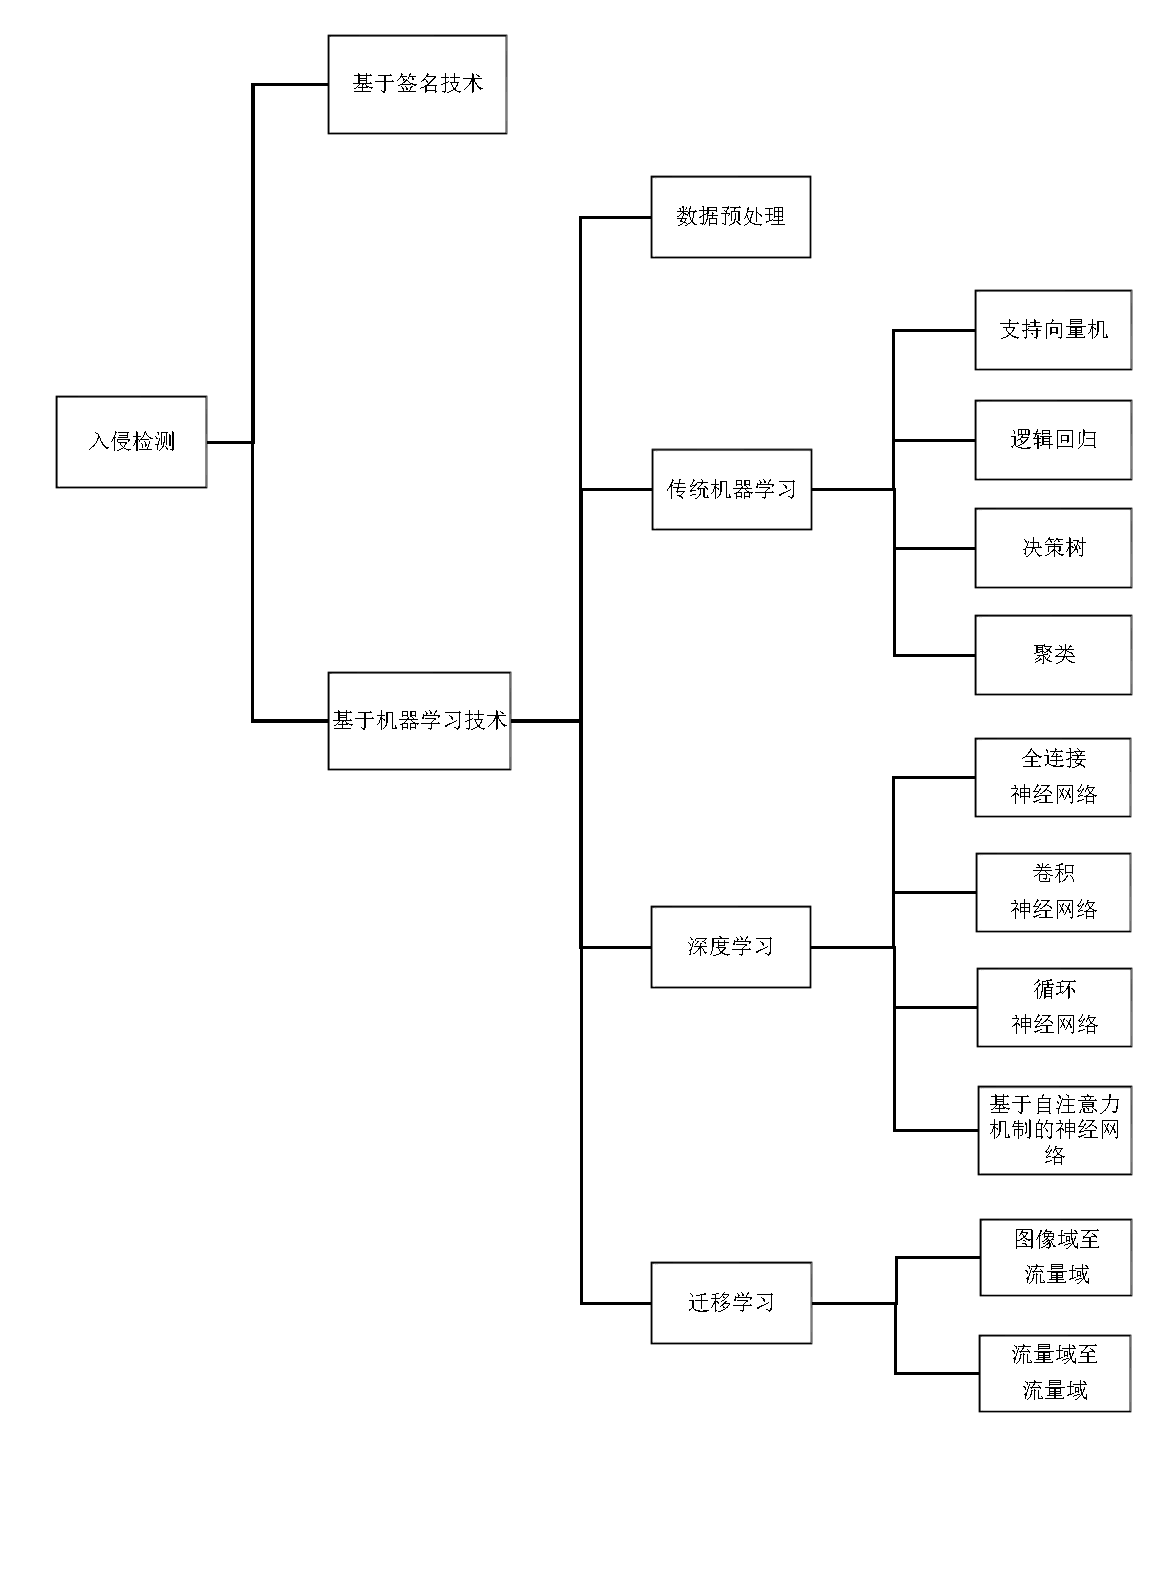
\includegraphics[width=.8\linewidth]{img/review.pdf} % 插入SVG图片
\caption{网络入侵检测方法分类}
\label{fig:research_review} % 子图的标签,用于交叉引用
\end{figure}%


\subsection{基于签名的网络入侵检测}
在基于签名的网络入侵检测系统中最重要的是签名数据库,该数据库由人工或机器根据已知的攻击模式提取特征并进行存储。入侵检测系统会对传入网络中的每一个数据包进行签名比对,一旦发现数据包特征与签名数据库中的特征匹配,入侵检测系统就会采取相应的防御措施。该方法广泛应用于商业防火墙软件中。在实际应用时,其灵敏度可根据实际情况进行调整,当设置为最高灵敏度时,虽然准确率最高,但会产生大量的误判。通过算法选择合适的签名,选出的签名可以保证在满足准确度要求的同时减少误报\cite{10.3390/app12020852}。基于签名的入侵检测技术可与基于机器学习的入侵检测相结合。使用蜜罐捕获网络攻击,随后使用机器学习分析捕获的流量,识别潜在恶意流量,对恶意流量实时生成签名并存储到数据库中,不断提高入侵检测系统的防御能力\cite{10.1007/s00521-019-04187-9}。
\subsection{机器学习数据预处理方法}
机器学习模型的性能上限由模型所学习数据的质量决定。为了保证模型能有效地从数据中学习,原始数据需要进行一系列预处理,从而转化为干净、格式统一的数据以便模型学习。原始数据分为结构化数据和非结构化数据。前者以表格形式呈现,有定义清晰的字段;后者没有固定格式,图像文字等属于此类。

在网络入侵检测任务中,结构化数据对应于通过指定算法抽取出的流量统计特征,而非结构化数据对应于原始的二进制网络流量数据。为提升机器学习中模型的学习效果以下是常用的数据预处理方法:
\begin{enumerate}
    \item 数值标准化。网络入侵检测中常用一种方法是最大最小值标准化方法,即将数值均匀地映射到[0,1]区间\cite{XAQY202212003,JSGG202206032,10.1016/j.csi.2023.103808,10.1080/21642583.2024.2321381,10.1109/ACCESS.2023.3251354}。另一种常见的方法是将样本各个属性转化为方差为1,均值为0的正态分布\cite{10.1016/j.ins.2021.03.060,10.1016/j.jksuci.2022.10.019}。对于分布范围很大的数据,取对数也是一种有效的标准化方法,可对数据范围进行显著压缩\cite{10.7717/peerj-cs.721}。
    
    \item 文字类型数据处理。网络流量特征中除了数值类型外,还包含文字类型数据,为方便处理此类数据,常使用的独热编码将其转换为稀疏二进制向量\cite{XAQY202212003,JSGG202206032,10.1016/j.csi.2023.103808,10.1016/j.measen.2022.100612,10.1016/j.knosys.2021.106798}。另一种方法是将文字类型转化为整数\cite{10.1016/j.simpat.2019.102031,10.1109/ICCSP48568.2020.9182099}。

    \item 对于网络数据包的负载部分,由于长度不同,可使用n-gram进行特征提取,该方法可将变长数据转化为定长向量\cite{10.1016/j.cose.2023.103171}。
    
    \item 网络流量的特征维度很高,对数据进行降维有助于提升模型表现,减少模型在学习过程中的过拟合现象。SelectKBest是一种常用特征选择方法,集成于scikit-learn库中,通过定义好的评分函数计算各个特征的重要性,以此选择最重要的k个特征实现降维\cite{10.1080/21642583.2024.2321381}。此外也可定义分数的阈值以选择最重要的特征\cite{10.1016/j.cose.2020.102062}。主成分分析是另一种根据阈值进行特征选择的方法,其选择方差最大的特征进行保留,从而将高维度数据投影至低维度\cite{10.1016/j.jksuci.2022.10.019}。计算数据各个分量之间的相关矩阵并剔除与目标变量(数据的类别)不相关或者彼此强相关的分量可以有效降维\cite{10.3390/math10030530}。自动编码器,也可以进行数据降维\cite{10.1016/j.knosys.2021.106798}。启发式算法也可进行特征选择,好的特征选择可以得到好的分类结果,于是可以将k近邻算法聚类效果作为评估函数,以选择最优特征子集\cite{10.1016/j.future.2020.07.042}。决策树算法如XGBoost 在进行分类时,实际上也实现了特征选择\cite{10.1016/j.comcom.2022.12.010,10.1016/j.icte.2020.03.002}。

    \item 网络流量数据存在显著的类别分布不均衡问题,即通常正常类别的样本数远大于异常类别样本数。直接在不平衡数据集上训练模型会缺少对小样本流量类别的识别能力,为重新平衡数据集可使用SMOTE(Synthetic Minority Over-sampling Technique)方法,通过对邻居样本采样合成新数据实现过采样\cite{PMID:34138657,10.7717/peerj-cs.721}。也可使用聚类增强过采样的效果\cite{XAXB202306010}。
    
\end{enumerate}
\subsection{基于传统机器学习的网络入侵检测}
\subsubsection{基于支持向量机的入侵检测}
支持向量机(Support Vector Machine, SVM)是一种监督学习方法。其核心思想是寻找最优超平面,该超平面能最大化不同类别数据之间的距离,理想情况下,不同类别之间的数据可以由一个超平面完美分隔开,但实际应用中数据分布较为复杂,并不是线性可分的。SVM通过使用核函数将样本映射到更高维度的空间,以获得更好的数据分布。样本个数是$n$的SVM在训练阶段的时间复杂度为$O(n^3)$,在处理网络入侵数据时可能成为性能瓶颈,可使用孪生支持向量机加快优化速度\cite{10.1109/ACCESS.2023.3251354}。

支持向量机在20年前就已经被应用到了入侵检测系统中\cite{10.1007/978-3-540-45235-5_73}。近年来使用支持向量机的入侵检测,都是将其与其他技术相结合提高支持向量机的性能,如使用高斯混合模型进行修正\cite{10.3390/electronics12040930},支持向量机可以用来替换深度学习中的softmax实现更好的分类效果\cite{PMID:37960661}。
\subsubsection{基于逻辑回归的入侵检测}
逻辑回归是机器学习中最简单最常用的模型,可根据输入变量判断其所属类别的概率。解决二分类问题时使用sigmoid函数,多分类问题则使用softmax函数。逻辑回归的最优参数常通过使用最大似然估计 得到。

入侵检测任务中可以使用其他启发式算法优化参数,如采用人工蜂群算法对逻辑回归的参数进行优化\cite{10.1016/j.csi.2023.103808}。偏最小二乘回归也可与逻辑回归进行结合,其具体分类流程是先对自变量进行降维,然后再用逻辑回归进行分类预测\cite{10.1007/978-981-33-4922-3_10}。
\subsubsection{基于决策树的入侵检测}
决策树由有向边和节点组成,节点分为两类,内部节点代表一种属性,叶节点代表具体类别。使用决策树对数据进行分类时,从根节点开始,数据都会根据每个内部节点对应的属性进行逐步划分,直至到达叶节点,即被划分为具体某一类别。对决策树进行模型集成,就可得到梯度提升决策树、随机森林等模型。

基于决策树的方法与其他机器学习方法进行结合,可克服单一模型的局限性。支持向量机很难用于解决多分类问题,将支持向量机嵌入到决策树内部结点中就可以解决入侵检测中的多分类问题\cite{10.1109/ACCESS.2023.3251354}。在数据集UNSW-NB15\cite{10.1109/MilCIS.2015.7348942}上进行数据降维后基于AdaBoost的决策树模型比简单的多层感知机或支持向量机效果要好\cite{10.3390/math10030530}。同时,在KDDCUP-99数据集上的研究,也表明决策树的性能优于逻辑回归和支持向量机\cite{10.1155/2021/6634811}。与支持向量机类似,决策树也可用于替代神经网络的softmax层以实现分类\cite{PMID:38339756}。对于多分类问题,也可以由不同的决策数分阶段进行决策,可以由两个决策树分别判断是否为恶意流量以及恶意流量对应的具体类别,然后由第3个决策树综合前两个决策树的分类结果输出最终分类结果\cite{10.3390/fi12030044}。

在进行集成学习的决策树模型上,可以使用其他方法进行二次集成,其中使用装袋法对集成了50个梯度提升机进行二次集成效果最好\cite{10.1016/j.eswa.2022.119030}。
\subsubsection{基于聚类的入侵检测}
聚类属于无监督学习即不需要样本的类别标签只需要样本特征,最基础的聚类算法是k均值聚类,其思想是通过迭代寻找若干中心点,每个中心点对应一种类别,最终使样本到所属中心点的距离最小。另一种实现聚类的方法是密度峰值聚类,但对于入侵检测这一种不均衡的数据集需要对其中密度峰值点的选择方法进行改进,让模型更重视稀疏区域\cite{10.1016/j.sysarc.2021.102212}。

对网络流量进行分类时,无监督聚类方法往往与其他有监督方法组合使用。聚类方法可以用在模型前端,使用k均值聚类进行第一步预分类,然后在每个聚类结果上分别训练随机森林分类器,这本质上也是一种模型集成方法\cite{10.1016/j.measen.2022.100612}。聚类也可以用在模型中间部分,分别对降维后的正常类别数据和异常类别数据进行两次聚类,然后将样本本身与距其最近的正常聚类中心和异常聚类中心组成二维数据,再使用卷积神经网络进行分类\cite{10.1016/j.knosys.2021.106798}。流量数据的特征分布较为复杂,在低维空间是线性不可分的,与支持向量机类似,可使用核函数,将其映射至容易线性可分的高维空间,使用多个核函数,可以让这一过程更简单\cite{10.1007/s13042-020-01253-w}。聚类的初始中心选择也非常关键,计算半相同(部分特征相似)实例集可以得到更好的聚类中心\cite{10.1016/j.cose.2020.102062}。除了通过不断迭代优化训练中心,也可以通过计算隶属函数确定某一样本是否属于已知集群以实现无监督聚类\cite{10.1007/s10699-019-09589-5}。神经网络也可应用到聚类过程中,为每个聚类中心配置一个神经网络,由该神经网络计算样本是否属于该类别可实现聚类\cite{10.1109/INFOCOM42981.2021.9488690}。

\subsubsection{传统机器学习存在的问题}
传统机器学习存在一定的局限性,特别是网络入侵领域,以下是对传统机器学习缺点的总结。
\begin{enumerate}
    \item SVM。SVM的性能很大程度上取决于核函数的选择,当更换数据集或数据集增加了新特征时,对模型进行调整较为困难。且SVM被设计用于二分类问题,异常网络流量可能有多个类别,这就需要设计多个SVM解决多分类问题,需要较多的计算资源。
    \item 逻辑回归。逻辑回归是一种线性模型,网络入侵检测中存在非线性特征,逻辑回归很难捕获复杂的攻击模式,其性能较差。
    \item 决策树。传统决策树算法,每个节点的特征选择与节点分裂都是根据整个数据集得到的,网络入侵检测中需要实时更新模型,而设计在线学习的决策树算法较为困难。另外,与SVM类似,决策树的结构与数据集密切相关,添加特征或更换数据集决策树往往会失效。
    \item 聚类。聚类是无监督的,识别每个簇代表的行为,需要进行额外的分析。在网络入侵检测中,由于数据不均衡,攻击流量可能会被视为噪音而被忽略。许多数据集提供了标签,而聚类方法是无监督的,并没有充分利用这些信息,其生成的模型效果较有监督模型差。
\end{enumerate}

深度学习是机器学习的一种,部分解决了上述存在的问题。深度学习在网络入侵检测领域的进展如下。

\subsection{基于深度学习的网络入侵检测}
\subsubsection{基于全连接神经网络的入侵检测}
多层感知机(Multilayer Perceptron,MLP)是一种人工神经网络,由一个输入层,多个隐藏层,以及一个输出层组成,两个相邻层之间的神经元相互连接,连接具有权值,每个神经元将连入它的连接加权求值,再使用非线性函数进行激活,激活后的值送入下一层。MLP是一种基础的神经网络架构,可用于监督学习任务,通常使用反向传播算法训练参数。

使用具有4个隐藏层,每个隐藏层具有100个节点的深度神经网络在KDDCUP-99数据集上具有最高性能,优于传统机器学习\cite{10.1049/iet-ifs.2018.5258}。


\subsubsection{基于卷积神经网络的入侵检测}
卷积神经网络与前一节所述的多层感知机相似,是对生物感知视觉方式的模仿,层与层之间没有全连接,而是使用卷积实现局部连接以及权值共享。一些数据集上相似的属性往往会放在相邻的位置,这就为使用卷积神经网络进行建模提供了方便。

随着ImageNet\cite{10.1109/CVPR.2009.5206848}数据集的提出,计算机视觉领域的神经网络架构研究取得了很多新的进展,因此只要将流量数据转化为图像,就可将用于视觉的网络架构应用到流量检测中。其中一种方法是将统计特征离散化转为二进制比特,然后将每8个二进制比特压缩为256灰阶像素,以此组成8×8的灰度图像使用ResNet等网络进行分类,该方法在NSL-KDD\cite{10.1109/CISDA.2009.5356528}数据集并未取得最好效果,但其优点在于无需进行特征选择\cite{10.1007/978-3-319-70139-4_87}。在将流量转化为图像的过程中,也可以不进行离散化,而是选择生成像素更多的图像\cite{PMID:34138657}。

除了转化为图像,也可使用一维卷积神经网络对流量数据直接进行分类。在此过程中,网络参数的设置非常重要,一种可行的解决方案是使用启发式算法进行优化,如粒子群算法对网络的结构进行搜索\cite{10.1016/j.ins.2021.03.060}。其他启发式算法如遗传算法也能进行网络搜索,搜索出的最优网络结构包含跨层连接\cite{10.1016/j.future.2020.07.042}。若不进行模型搜索,一种近似方法是使用多种尺寸的卷积以实现模型对流量的多尺度建模\cite{10.1016/j.future.2021.10.018}。

卷积网络除了对单个样本进行建模外,也可以进行局部时序建模\cite{10.7717/peerj-cs.721}。
\subsubsection{基于循环神经网络的入侵检测}
循环神经网络是用来进行时序建模的主流模型,传统的前馈神经网络如多层感知机和卷积神经网络,这些模型的输入尺寸都是固定的,无法处理变长的序列,而循环神经网络则将时序信息串行化,依次处理每一时刻的信息,且在处理时维护一个内部状态以记录之前的输入信息,实现对时序数据的感知。

最简单的结构是只使用循环神经网络,然后接全连接层\cite{10.1109/ICCSP48568.2020.9182099}。除了使用全部数据集中给出的特征,也可进行特征选择,只使用精简特征进行分类\cite{10.1016/j.comcom.2022.12.010,10.1016/j.icte.2020.03.002}。进行特征选择后,模型效果会好于使用全部特征且计算量更少内存占用更低\cite{10.1016/j.comnet.2023.109662}。使用去噪自编码器也可为循环神经网络提供降维后的特征\cite{XAXB202302002}。考虑网络流量类别的极度不均衡,可以由两个级联的递归神经网络进行分类,其中第一个检测是否为常见攻击类型,第二个检测是否为少见攻击类型\cite{10.1016/j.simpat.2019.102031}。

循环神经网络(Recurrent Neural Network,RNN)也可以与卷积神经网络搭配使用。常见方法是先使用若干层卷积神经网络提取网络流量的局部特征,然后再使用循环神经网络,提取网络流量的全局时序特征。不超过三层时,循环神经网络的层数越多效果越好,且使用长短期记忆网络(Long Short-Term Memory,LSTM)的效果最好,其次是门控神经单元(Gated Recurrent Unit,GRU),最差的是标准的RNN\cite{10.1109/ICACCI.2017.8126009,10.1016/j.comcom.2022.12.010}。为了充分利用这三种类型网络的差异性,可以使用并行结构将流量特征使用三种网络分别建模,然后进行降维,降维后再进行特征融合\cite{10.1016/j.compeleceng.2022.108156}。除了这三种基本结构,单循环单元(Simple Recurrent Unit,SRU)也可用于入侵检测,该神经单元的特点是采用了跳接思想以避免梯度消失,工业数据集上该方法确实优于GRU和LSTM\cite{10.1016/j.compeleceng.2021.107049}。在KDDCUP-99数据集上先使用三层卷积神经网络进行数据包的特征提取,然后再使用循环神经网络进行建模时发现:循环神经网络中长短期记忆网分类效果好,门控神经单元速度快,可以使用混合结构,在网络中的不同层次依次使用这两种网络,以实现更好的性能,考虑到循环神经网络的单向性,也可以由两层不同方向的网络对接起来,以实现双向时序建模\cite{10.1016/j.jksuci.2022.10.019}。对于这种具有复合结构的网络而言,超参数设置仍然很重要,因此可以通过使用遗传算法,对网络的超参数进行搜索\cite{10.1007/s11042-021-11271-7}。
最后得到分类结果,除了使用softmax或sigmoid函数计算外也可使用随机森林或支持向量机得出\cite{10.1016/j.compeleceng.2022.108156}。使用基于RNN的网络,可以构建自动编码器,根据重建结果与实际结果的差异值可判断是否为异常流量及恶意流量\cite{10.1109/TCAD.2020.3012749}。
\subsubsection{基于自注意力机制的入侵检测}
基于自注意力机制的神经网络模型中,最经典的是Transformer\cite{NIPS2017_3f5ee243},该模型主要由两部分组成,分别是多头自注意力机制以及其后的多层感知机,自注意力机制为该模型提供了全局建模能力以及对输入的灵活适应性。Transformer由两部分组成,分别是编码器和解码器。

最简单的方法是直接使用Transformer的原方案,对解码器的输出使用softmax函数得到样本对应的类别,该方案在相同推理时间的情况下,优于RNN和SVM\cite{10.1109/ACCESS.2022.3182333}。在仅使用编码器的情况下,其效果也优于RNN\cite{10.1016/j.comnet.2023.110072}。提取统计特征之后的流量数据,本质上是表格数据,因此可以使用TabNet进行分类\cite{PMID:37844095}。FlowTransformer框架对该Transformer应用到入侵检测中进行了探索,发现入侵检测任务比较简单,小模型与大模型的区别较小,影响模型性能的关键在于分类器的选择\cite{10.1016/j.eswa.2023.122564}。对卷积神经网络而言可将流量转化为图像,然后使用图像分类网络判断流量,对Transformer也是如此,但分类效果不如原生网络\cite{10.1109/ACCESS.2022.3200034}。网络流量有两种特征,分别是原始字节流和统计特征,可将这两种特征进行融合,对流量数据统一进行特征提取与分类\cite{10.1145/3511808.3557549}。使用多层感知机对传入Transformer的流量特征提前进行初步编码,可改善模型表现\cite{10.1016/j.cose.2023.103171}。对Transformer进行改进可以将其与卷积神经网络结合,先使用简单的卷积神经网络进行初步训练,将训练后的卷积层与Transformer相连,实现细粒度建模,在不同数据集上均优于传统模型\cite{10.1007/s11042-022-14121-2}。除了传统卷积,也可使用时序卷积以实现对局部时序信息的初步建模,该方法可以提升Transformer的性能\cite{10.1109/ACCESS.2022.3175516}。该方法也可与传统机器学习方法相结合,先使用决策树判断流量是否为恶意流量,然后再使用Transformer判断恶意流量具体的类别,级联后的方案比单独使用其中一种效果更好\cite{10.1109/ICDMW58026.2022.00081}。

\subsubsection{深度学习存在的问题}
上述四种深度学习方法存在一定的局限性,以下是对深度学习缺点的总结。
\begin{enumerate}
    \item 网络流量数据是时序数据,MLP缺乏时序建模能力。
    \item 将流量数据统计特征转化为图像会丢失信息。由于其感受野的局部性,单个网络流量中相距较远的两个特征的组合,需要通过多层卷积才能实现特征提取。
    \item 循环神经网络处理在处理长序列时存在梯度消失或梯度爆炸问题。
    \item 数据集中给出了每个特征对应的描述,模型并未充分利用。
\end{enumerate}

\subsection{迁移学习}
迁移学习,可以大体分为四类。第1类以TrAdaBoost\cite{10.1145/1273496.1273521}为代表,从源数据集中找到对目标任务有帮助的样本,从而实现前移学习。第2类方法以\cite{10.1109/TNN.2010.2091281}为代表,尝试将原数据集和目标数据集映射到同一个特征空间中,在映射过程中尽量减少数据信息的损失的同时,尽量让映射后的分布相同。第3类是在神经网络上进行迁移学习,其核心思想是重新利用已经在原数据集上训练好的参数,对源数据集上训练好的网络稍作修改即可用作目标数据集,如预训练的BERT\cite{10.18653/v1/N19-1423}。第4类是使用对抗性技术\cite{NIPS2006_b1b0432c}。当辨别器无法区分特征是来源于目标数据集还是原数据集,这说明了编码器提取的特征是同分布的。
\subsubsection{基于图像转换的网络流量迁移学习}
ImageNet是一个图像分类任务的数据集,它作为一个统一的标准,推进了人们对更有效网络结构的探索。在此任务上人们有丰富的方法与模型,如果能将网络流量数据转为图像,那就只需图像预训练模型即可完成迁移学习。TL-NID就是这么做的,它使用min-max标准化,然后将一维的序列折叠成二维的灰度图像再使用预训练的VGG-16实现迁移学习,效果比用决策树和随机森林好\cite{10.23919/ICITST51030.2020.9351317}。对于一些字符串类型的数据可以将其转化为独热编码\cite{10.1109/ACCESS.2020.2972627}。除了使用统计后的数据,也可以直接将二进制数据包按固定长度截断,把每个字节看成8-bit的灰度值,直接转化为图像,但预训练效果较差,可能是由于生成的图像与真实图像存在显著不同\cite{10.3390/info13120553}。直接使用灰度图像不利于特征的提取,在之前的基础上有人使用卷积将一维特征序列映射为RGB图像,然后使用模型集成的方法对流量进行判断\cite{10.1109/ACCESS.2022.3233775}。流量特征也可以通过三种降维方式(PCA、t-SNE和KPCA)生成三个通道对应彩色图像的RGB\cite{10.1016/j.future.2021.07.015}。TDL-IDS\cite{10.1109/GLOBECOM48099.2022.10001267}则是充分考虑了数据包之间的时序关系,采用LSTM进行建模,在NSL-KDD上训练后,冻住部分隐藏层然后在AWID数据集上微调。另一种迁移学习的方法则是先使用卷积神经网络学习粗略的特征,然后在第二阶段冻住网络,在后面添加新的网络实现对目标数据集上特征的准确提取\cite{10.1109/ICBDA.2019.8713213}。

\subsubsection{基于网络流量特征的迁移学习}
除了把数据转化为图片,然后使用图像分类,对网络进行流量分类也可以直接对流量进行处理。使用普通的全连接层搭建神经网络进行迁移学习,具体方法是先在原数据集上进行训练,然后重置Softmax层再在目标数据集上进行微调,但该实验提出的方法只能处理同样结构的数据\cite{10.1109/SMARTCOMP.2019.00031}。另一个方法是优化两个矩阵,使源数据集和目标数据集都可以通过投影矩阵投影到一个相同的子空间\cite{10.1109/MILCOM.2017.8170749}。从原始的二进制网络流量出发,对不同数据集提取相同格式的特征,然后使用卷积神经网络,在其中一种上进行训练,随后冻结训练好网络中的上半部分再在定目标数据集上对训练好的网络进行微调,可以实现迁移学习 \cite{10.1016/j.eswa.2022.118641}。

\subsubsection{迁移学习存在的问题}
上述两种迁移学习存在一定的局限性,以下是对迁移学习缺点的总结。
\begin{enumerate}
    \item 将网络流量转化为图像时,生成的图像与自然图像不同,可能会导致模型难以准确提取数据的特征,限制模型性能。
    \item 将流量数据统计特征转化为图像,实际上进行了升维,需要更大的存储空间,转化过程也需要消耗大量计算资源。
    \item 直接进行迁移学习时,若数据集的格式发生变化,需要重置投影层或使用新的投影矩阵。这些抛弃的参数中含有模型里学到的信息,迁移过程中,这些信息并没有被迁移到新模型中。
\end{enumerate}

\subsubsection{研究挑战与科学问题}
根据国内外研究现状,入侵检测领域的研究挑战是:
\begin{enumerate}
    \item 网络流量数据中存在多种模态(数值、文本等)的数据,如何如何充分融合这些数据以及描述信息对提升模型检测能力较为重要,而当前缺少合适的融合方法。
    \item 公共数据集与现实存在区别,当在实际环境中部署公共数据集训练得到的模型,其检测性能会下降。基于模型的迁移学习中存在损失,这会降低迁移效果。减少信息损失对模型设计以及迁移方法提出了更高要求。
\end{enumerate}

针对上述挑战,本文要解决的科学问题是如何解决公共数据集与实际数据的差异导致模型性能下降的问题。

\section{本文主要研究内容}
\label{sec:Research content for this paper}
\subsection{研究目标}
针对本文在入侵检测领域要解决的科学问题,研究目标如下:
\begin{enumerate}
    \item 设计新的映射方法将端口值、协议类型等字段进行更合理的映射。该映射与数据集无关,与上述字段的含义有关,减少了迁移时模型参数的信息损失。
    \item 利用Transformer的多模态建模能力,将数据集中的文字描述部分融入模型的特征提取与分类过程中,实现语言信息辅助建模,提高分类准确率。将建模后的信息进行时序特征提取,进一步提高分类的准确率。
    \item 使用通用模型,在不同数据集之间进行迁移学习,在迁移过程中减少模型的修改,尽可能保留已学习的参数。同时相比传统迁移学习方法,使用通用模型的分类方法具有更高准确率。
\end{enumerate}

\subsection{具体工作}

从上述研究目标出发,本文构建的多模态通用入侵检测系统如下图示,其主要由三个部分构成,分别是数据预处理,模型训练与推理,结果批量导出。
\begin{enumerate}
    \item 数据预处理部分的工作主要有两部分,对于文字部分需要将文本转化为对应的向量,对于数值部分则需要通过一定的算法将其转化为较小的分布范围,帮助模型学习其中的特征。同时将数据集中描述部分转化为句子表征向量。
    \item 利用Transformer的多模态能力在位置编码部分引入语义信息。
    \item 构建通用编码器同时引入以及进行时序建模,在建模过程中引入数据集中的表征向量,提高模型对不同数据集的适应性减少迁移学习时的信息损失。

\end{enumerate}

\section{论文组织结构}
\label{sec:Paper organization structure}
论文共有六个章节,组织结构如下:

第1章 绪论。简要说明了网络入侵检测领域所研究的内容,以及国内外对于机器学习在入侵检测中的最新研究进展,总结了当前研究方法存在的局限性,并进一步说明本文研究的内容以及提出的方法。

第2章 数据预处理与数据增强。介绍所用数据集并对数据集的特点进行分析,根据分析结果对数据集给出了相应的预处理方法以及数据增强方法。

第3章 基于多模态的入侵检测。提出了一种基于Transformer的通用入侵检测模型,说明了引入语言信息辅助建模的具体思路,介绍了实验平台设置以及入侵检测中常用的评价指标,在CIC-IDS2017数据集上进行了相关实验并对位置编码进行可视化分析。

第4章 基于时序建模的入侵检测。在多模态模型的基础上进行时序建模,将实验结果与近期入侵检测领域的研究进展进行了对比并对时序上的注意力进行了可视化分析。

第5章 基于迁移学习的入侵检测。给出了将时序多模态模型迁移至目标数据集上的实现方法,并使用两个数据集进行试验,比较了两种迁移学习方法。

第6章 总结与展望。总结了本文提出的多模态通用检测方法并分析了方法存在的不足,给出了未来可能改进的方向。

\chapter{数据预处理与数据增强}
数据是机器学习三要素之一,它决定了机器学习算法能达到的上限。对数据进行预处理与增强能有效提高模型性能,使用数据增强可扩充数据集防止过拟合。

入侵检测任务的目标是找到一种函数,该函数对于给定的序列$ \mathbf{X} = (\mathbf{x}_1, \mathbf{x}_2, \ldots, \mathbf{x}_n) $可以输出该序列每一个位置对应的类别$ \mathbf{Y} = (\mathbf{y}_1, \mathbf{y}_2, \ldots, \mathbf{y}_n) $。序列中的每一项代表一个数据包原始数据,每个数据包对应的信息是以二进制比特流形式呈现。由于二进制比特流不是定长的,且现在网络流量中大部分数据载荷都经过加密处理,如果直接分析加密的流量很难得到有效信息,且占较大存储空间。

因此部分数据集以统计特征形式给出而不是原始网络流。即采用统计学方法提取网络流量数据的统一特征,将变长的数据流转化为定长的统计特征向量。于是上文所说的给定序列中每一项$\mathbf{x}_i$就代表一个维度固定的向量。这些向量中既包含数值信息(如数据包的长度),也包含文本信息(如数据包的类型,TCP还是UDP)。包含文本信息的向量无法由机器学习模型直接处理,且一些数值分布范围广,给机器学习造成了困难。

本章提出的预处理方法,解决了上述问题。首先将数值替换文本,使该向量变成统一类型的向量,同时建立嵌入向量表,数值即为嵌入向量表中的索引。然后对原向量中的数值部分进行重新映射,将分布范围过大的数据项映射为分布范围较小的数据项,以便模型处理。

对网络流量进行时序建模时,还需要对流量数据进行切片。对切片后的数据进行数据增强,还需考虑维持原有数据分布及数据特点。
\section{入侵检测数据集}
研究中使用的数据集有两个,分别是KDDCUP-99和CIC-IDS2017\cite{Sharafaldin2018TowardGA},前者主要用于验证迁移学习性能,后者用于验证模型性能。
\subsection{KDDCUP-99数据集简介}

在入侵检测领域最基础的数据集是KDDCUP-99,这是一个竞赛数据集,该竞赛的任务是创建一个分类器以区分网络流量的好与坏。KDDCUP-99分为训练集与测试集,其中训练集包含七周的网络流量数据,有约500万条连接,测试集中包含两周的网络流量,大约包含200万条连接。每条连接指的是从tcp连接到释放连接的全部数据包序列。连接分为5个大类:
\begin{enumerate}
\item 正常流量:没有恶意的正常网络活动。
\item 拒绝服务(Denial-of-Service):发送大量无用信息,以耗尽服务器资源的网络活动。
\item 远程未授权访问(R2L):未经授权的用户通过远程访问获取资源,这种类型的网络流量通常用于窃取数据与破坏系统。
\item 本地未授权访问(U2R):攻击者试图在本地系统上获得超级用户的权限,一旦获取超级用户权限就可控制整个系统,并进一步进行攻击。
\item 探测(Probe):获取目标网络的当前状态,如开放端口以及正在运行的网络服务,识别可能存在漏洞,以方便进行下一步攻击。
\end{enumerate}

KDDCUP-99中的攻击类型分类情况如表\ref{table:kdd_attack_types}示,共7大类,15小类。标签数量如图\ref{fig:kdd99_category}示,可以看到拒绝服务流量最多,其次是正常流量,最少的是本地未授权访问。

\begin{table}[htb]
  \centering
  \caption{KDDCUP-99攻击类型总结}
  \begin{tabular}{p{0.15\linewidth}p{0.85\linewidth}}
    \toprule
    \textbf{攻击分类}& \textbf{具体类别}\\
    \midrule
    BENIGN & normal \\
    Denial-of-Service & back, neptune, smurf, teardrop, land, pod, apache2, mailbomb, processtable \\
    Probe & satan, portsweep, ipsweep, nmap, mscan, saint \\
    R2L & warezmaster, warezclient, ftp\_write, guess\_passwd, imap, multihop, phf, spy, sendmail, named, snmpgetattack, snmpguess, xlock, xsnoop, worm \\
    U2R & rootkit, buffer\_overflow, loadmodule, perl, httptunnel, ps, sqlattack, xterm \\
    \bottomrule
  \end{tabular}
  \label{table:kdd_attack_types}
\end{table}

\begin{figure}[htb]
\centering % 居中对齐子图
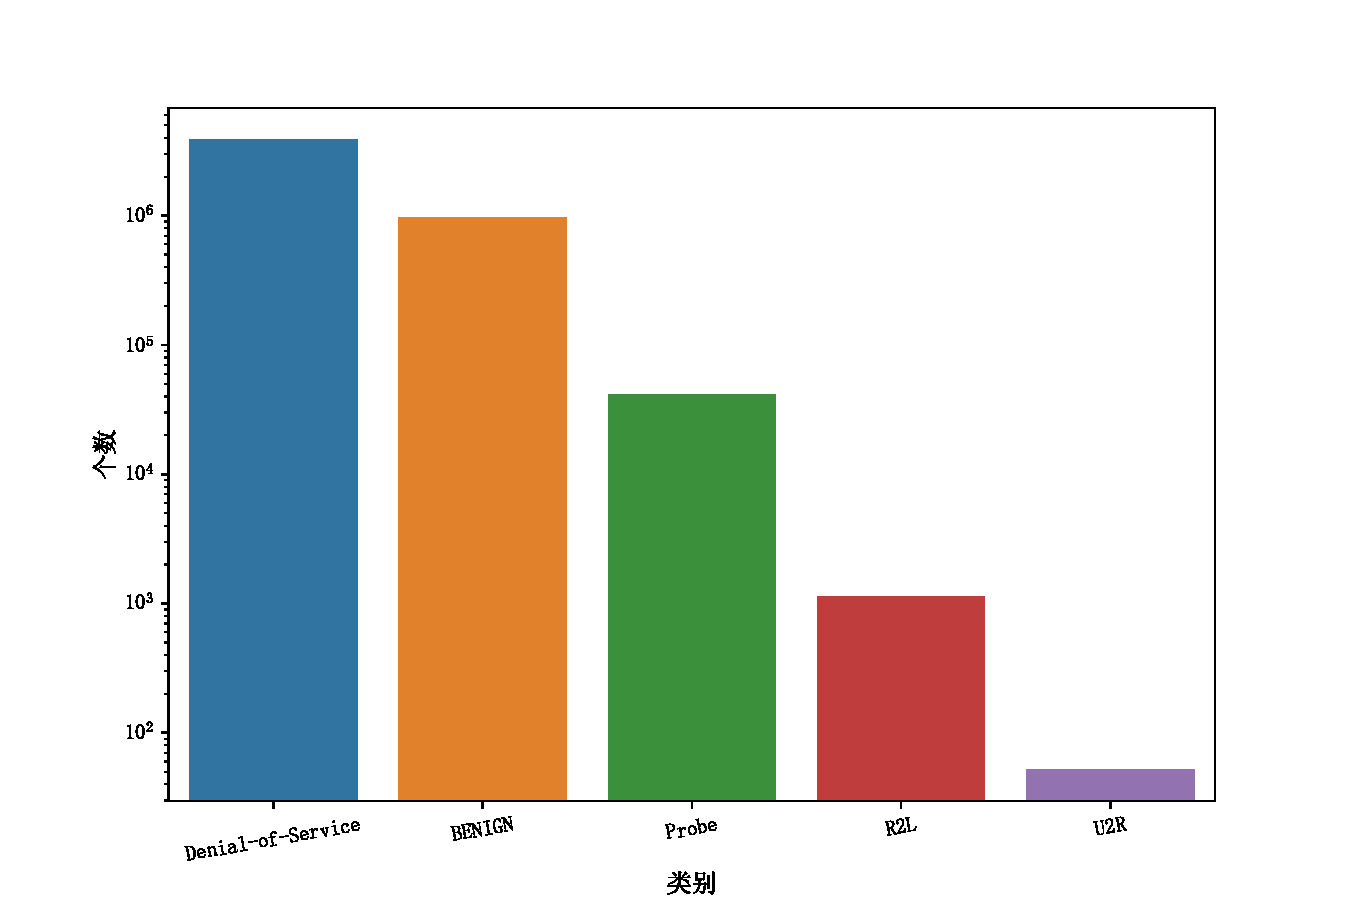
\includegraphics[width=.95\linewidth]{img/preprocessing/kdd99_category.pdf} % 插入SVG图片
\caption{KDDCUP-99类别分布}
\label{fig:kdd99_category} % 子图的标签,用于交叉引用
\end{figure}%

\subsection{CIC-IDS2017数据集简介}
CIC-IDS2017是另一个网络入侵检测领域常用的数据集,该数据集采集自5天的网络流量,既包含原始数据,也包含使用CICFlowMeter分析后的结果。数据集没有划分训练集与测试集,共3119345条数据。数据分为7个大类:
\begin{enumerate}
\item 正常流量:没有恶意的正常网络活动。
\item 暴力攻击:攻击者尝试用户名以及密码,通过认证从而获取权限。
\item 机器人网络:攻击者通过控制大量机器组成攻击平台,可对攻击目标产生巨大的攻击流量。
\item 端口扫描:识别当前网络开放的端口,确定服务器上正在运行的服务与应用。
\item 拒绝服务:攻击者建立大量半开连接从而消耗服务器资源,阻碍服务器对正常请求的响应。
\item 网络应用程序攻击:此类攻击主要指因程序设计不合理,导致服务器无法区分命令与数据的攻击类型,如各种注入攻击。
\item 未知类型:主要指难以确定的小样本攻击类型。
\end{enumerate}

CIC-IDS2017攻击类型分类情况如表\ref{table:cic2017_attack_types}示,共7大类,24小类。标签数量如图\ref{fig:cic2017_category}示,可以看到正常流量最多;其次是拒绝服务、端口扫描和暴力攻击,这些攻击类型本身就需要大量的攻击流量,然后是网络应用攻击和机器人网络,最少的是未知类型攻击,在对数坐标系下也显著少于其他类型。

\begin{table}[htb]
  \centering
  \caption{KDDCUP-99攻击类型总结}
  \begin{tabular}{p{0.2\linewidth}p{0.8\linewidth}}
    \toprule
    \textbf{攻击类型(大类)} & \textbf{攻击类型(小类)} \\
    \midrule
    BENIGN & BENIGN \\
    Brute-force-attack & FTP-Patator, SSH-Patator \\
    Botnet & Bot \\
    Denial-of-Service & DoS GoldenEye, DoS Hulk, DoS Slowhttptest, DoS slowloris, DDoS \\
    Web-Attacks & Web Attack – Brute Force, Web Attack – Sql Injection, Web Attack – XSS \\
    PortScan & PortScan \\
    Unknown & Infiltration, Heartbleed \\
    \bottomrule
  \end{tabular}
  \label{table:cic2017_attack_types}
\end{table}
\begin{figure}[htb]
\centering % 居中对齐子图
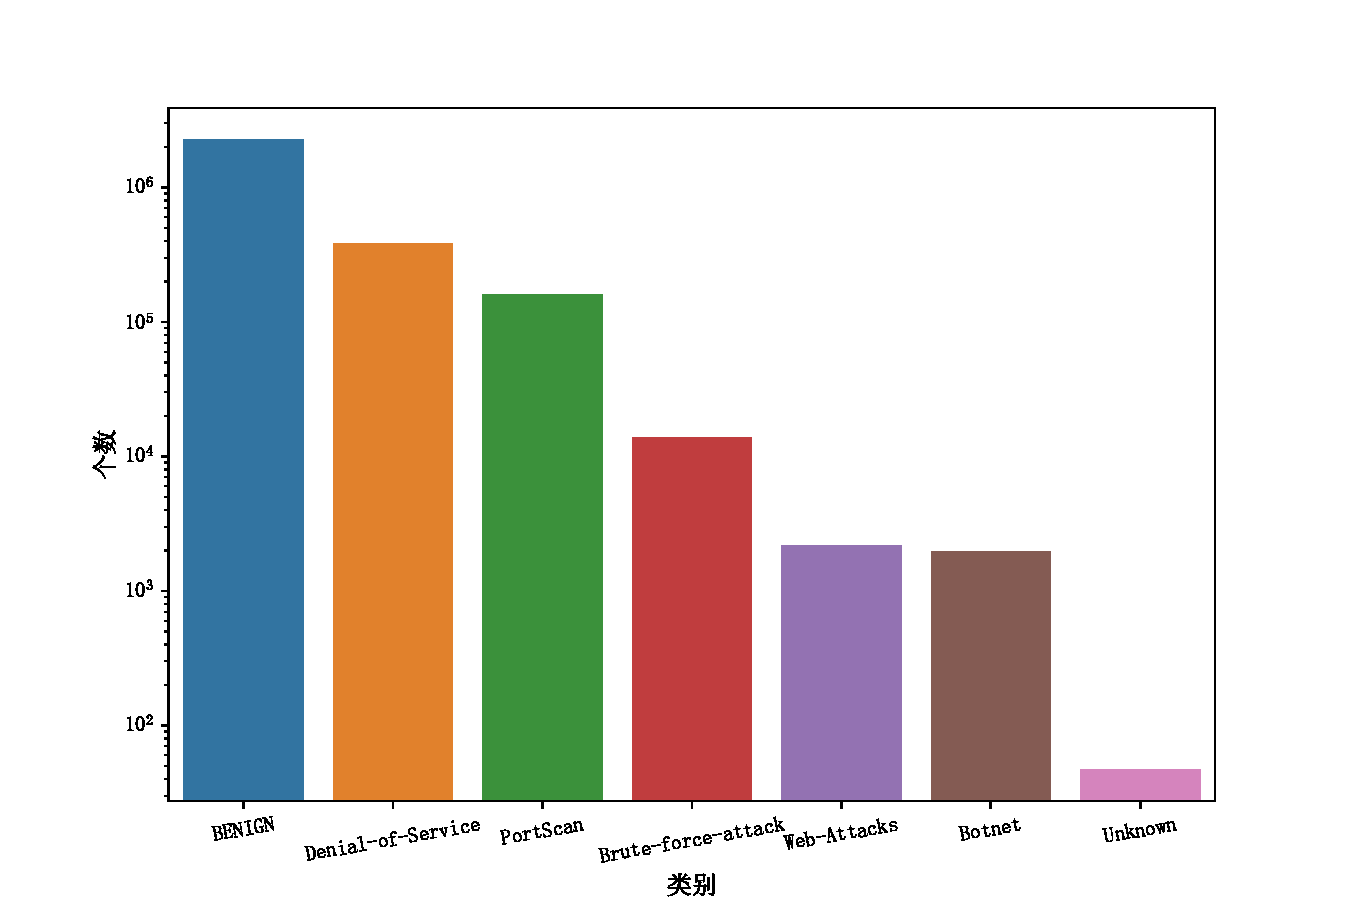
\includegraphics[width=.95\linewidth]{img/preprocessing/cic2017_category.pdf} % 插入SVG图片
\caption{CIC-IDS2017类别分布}
\label{fig:cic2017_category} % 子图的标签,用于交叉引用
\end{figure}%

\section{数据集格式}
网络入侵检测数据通常有两种格式,分别是原始捕获的二进制比特流以及通过如CICFlowMeter等网络流量分析工具初步分析后得到的统计特征,KDDCUP-99数据集只给出了统计特征,CIC-IDS2017数据集给出了这两者,为了形式统一,本研究仅使用流量分析工具得到的统计特征。
\subsection{KDDCUP-99数据集格式}
KDDCUP-99数据集是以逗号分隔符形式给出的,可以看作是一张表格,总共42列,前41列是连接的特征,最后一列是连接的类别,数据集共4898431行。第1行数据如下:
\begin{itemize}
\item \seqsplit{0,tcp,http,SF,215,45076,0,0,0,0,0,1,0,0,0,0,0,0,0,0,0,0,1,1,0.00,0.00,0.00,0.00,1.00,0.00,0.00,0,0,0.00,0.00,0.00,0.00,0.00,0.00,0.00,0.00,normal.}
\end{itemize}
这41列特征按数值类型可分为四类,分别是:表示是与否的二值类型、表示百分比的浮点类型、表示文本的字符串、表示个数的整数值,其中二值类型可看作特殊的百分比,41维特征划分如表\ref{table:kdd_feature_types}示。

\begin{table}[htbp]
\centering
\caption{数据类型分类}
\begin{tabular}{p{0.15\linewidth}p{0.7\linewidth}}
\toprule
\textbf{类型} & \textbf{名称} \\
\midrule
整数 & duration, src\_bytes, dst\_bytes, land, wrong\_fragment, urgent, hot, num\_failed\_logins, lnum\_compromised, lnum\_root, lnum\_file\_creations, lnum\_shells, lnum\_access\_files, lnum\_outbound\_cmds, count, srv\_count, dst\_host\_count, dst\_host\_srv\_count \\
\addlinespace
浮点或二值 & logged\_in, lroot\_shell, lsu\_attempted, is\_host\_login, is\_guest\_login, serror\_rate, srv\_serror\_rate, rerror\_rate, srv\_rerror\_rate, same\_srv\_rate, diff\_srv\_rate, srv\_diff\_host\_rate, dst\_host\_same\_srv\_rate, dst\_host\_diff\_srv\_rate, dst\_host\_same\_src\_port\_rate, dst\_host\_srv\_diff\_host\_rate, dst\_host\_serror\_rate, dst\_host\_srv\_serror\_rate, dst\_host\_rerror\_rate, dst\_host\_srv\_rerror\_rate \\
\addlinespace
文本 & protocol\_type, service, flag \\
\bottomrule
\end{tabular}
\label{table:kdd_feature_types}
\end{table}

整数类型含义指某种操作的次数包的个数长度等,将这类数值进行可视化如图\ref{fig:kdd99_bighist}示,可见其分布不均,大部分数值较小。

百分比类型含义指连接中某类连接占总连接的百分比或者某种操作是否成功,分别对二者类型百分比类型以及两者合并后的数值进行可视化分析,如图示\ref{fig:kdd99_samllhist},等于0与等于1的值最多。

文本类型包括协议类型,网络服务类型以及连接的状态。

\begin{figure}[htbp] % 创建一个新的figure环境
\centering % 居中对齐所有的子图

\subfloat[分布范围小的属性分布情况]{ % 插入第一个子图及其标题
\begin{minipage}{.5\textwidth}
\centering % 居中对齐子图
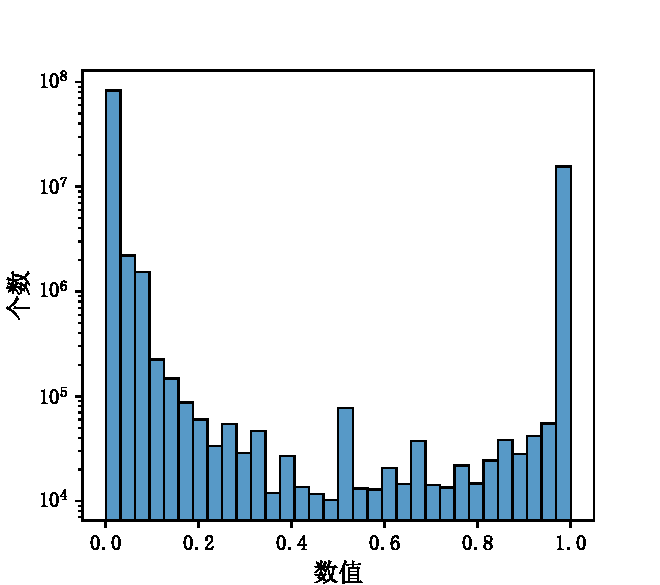
\includegraphics[width=1\linewidth]{img/preprocessing/kdd99_smalldata.pdf} % 插入SVG图片
\label{fig:kdd99_samllhist} % 子图的标签,用于交叉引用
\end{minipage}%
}
\subfloat[分布范围大的属性分布情况]{ % 插入第二个子图及其标题
\begin{minipage}{.5\textwidth}
\centering
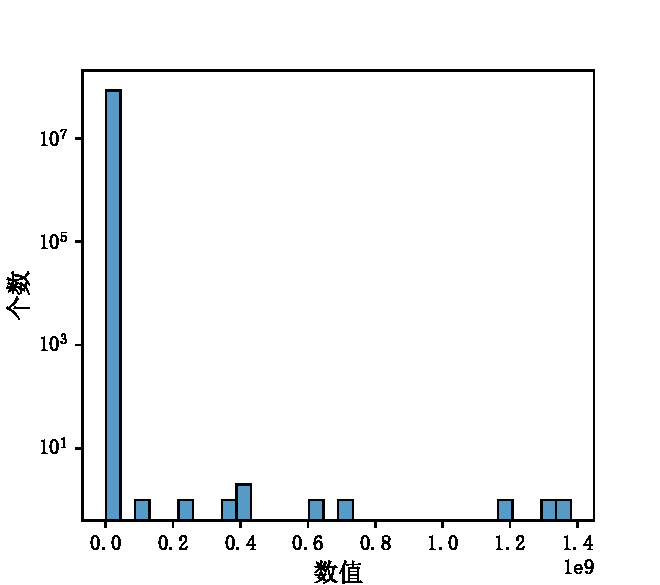
\includegraphics[width=1\linewidth]{img/preprocessing/kdd99_bigdata.pdf} % 插入SVG图片
\label{fig:kdd99_bighist}
\end{minipage}
}

\caption{kdd99数据(正数部分)分布直方图} % 四张图片作为整体的标题
\label{fig:kdd99_hist}
\end{figure}


\subsection{CIC-IDS2017数据集格式}

该数据集以逗号分隔符形式给出,有多个文件,总共85列,第1列是连接的特征码由连接双方的IP地址端口以及协议类型组成,有两列列名为“Fwd Header Length”重复的列,最后一列是连接的类别,其他的82列为连接特征。第1行数据如下:
\begin{itemize}
\item \seqsplit{192.168.10.5-8.254.250.126-49188-80-6,8.254.250.126,80,192.168.10.5,49188,6,03/07/2017 08:55:58,4,2,0,12.0,0.0,6.0,6.0,6.0,0.0,0,0,0,0,3000000.0,500000.0,4.0,0.0,4.0,4.0,4.0,4.0,0.0,4.0,4.0,0,0,0,0,0,0,0,0,0,40,0,500000.0,0.0,6.0,6.0,6.0,0.0,0.0,0,0,0,0,1,1,0,0,0.0,9.0,6.0,0.0,40,0,0,0,0,0,0,2,12,0,0,329,-1,1,20,0,0,0,0,0,0,0,0,BENIGN}
\end{itemize}
连接特征中的双方IP地址、时间戳无法用于分类。故可用于分类的特征有79列,按数值范围和类型可分为三类,分别是:表示索引的数值,最大值小于等于1的数值,最大值大于1的数值,79维特征划分如表\ref{table:cic2017_feature_types}示。

\begin{table}[htb]
\centering
\caption{数据类型分类}
\begin{tabular}{p{0.15\linewidth}p{0.57\linewidth}}
\toprule
\textbf{类型} & \textbf{名称} \\
\midrule
最大值大于1 & Flow Duration, Total Fwd Packets, Total Backward Packets, Total Length of Fwd Packets, Total Length of Bwd Packets, Fwd Packet Length Max, Fwd Packet Length Min, Fwd Packet Length Mean, Fwd Packet Length Std, Bwd Packet Length Max, Bwd Packet Length Min, Bwd Packet Length Mean, Bwd Packet Length Std, Flow Bytes/s, Flow Packets/s, Flow IAT Mean, Flow IAT Std, Flow IAT Max, Flow IAT Min, Fwd IAT Total, Fwd IAT Mean, Fwd IAT Std, Fwd IAT Max, Fwd IAT Min, Bwd IAT Total, Bwd IAT Mean, Bwd IAT Std, Bwd IAT Max, Bwd IAT Min, Fwd Header Length, Bwd Header Length, Fwd Packets/s, Bwd Packets/s, Min Packet Length, Max Packet Length, Packet Length Mean, Packet Length Std, Packet Length Variance, Down/Up Ratio, Average Packet Size, Avg Fwd Segment Size, Avg Bwd Segment Size, Subflow Fwd Packets, Subflow Fwd Bytes, Subflow Bwd Packets, Subflow Bwd Bytes, Init\_Win\_bytes\_forward, Init\_Win\_bytes\_backward, act\_data\_pkt\_fwd, min\_seg\_size\_forward, Active Mean, Active Std, Active Max, Active Min, Idle Mean, Idle Std, Idle Max, Idle Min\\
\addlinespace
最大值小于1 & Fwd PSH Flags, Bwd PSH Flags, Fwd URG Flags, Bwd URG Flags, FIN Flag Count, SYN Flag Count, RST Flag Count, PSH Flag Count, ACK Flag Count, URG Flag Count, CWE Flag Count, ECE Flag Count, Fwd Avg Bytes/Bulk, Fwd Avg Packets/Bulk, Fwd Avg Bulk Rate, Bwd Avg Bytes/Bulk, Bwd Avg Packets/Bulk, Bwd Avg Bulk Rate \\
\addlinespace
索引值 & Source Port, Destination Port, Protocol \\
\bottomrule
\end{tabular}
\label{table:cic2017_feature_types}
\end{table}

分布范围小于等于1的数值指连接中是否存在FIN、SYN、ACK等标识或者是表示某种占比,如图\ref{fig:cic2017_samllhist}示,可见其分布范围集中于0附近与1附近,实际上尽管某些属性表示占比,但这些属性只有0和1两个值,且0的个数远大于1的个数。

分布范围大的数值含义指某种操作的次数、包的个数、包的长度等,将这类数值进行可视化如图\ref{fig:cic2017_bighist}示,可以看出其分布不均,绝大多数数值较小,数据分布范围广。

索引的数值表示端口号或协议号。

\begin{figure}[htbp] % 创建一个新的figure环境
\centering % 居中对齐所有的子图

\subfloat[分布范围小的属性分布情况]{ % 插入第一个子图及其标题
\begin{minipage}{.5\textwidth}
\centering % 居中对齐子图
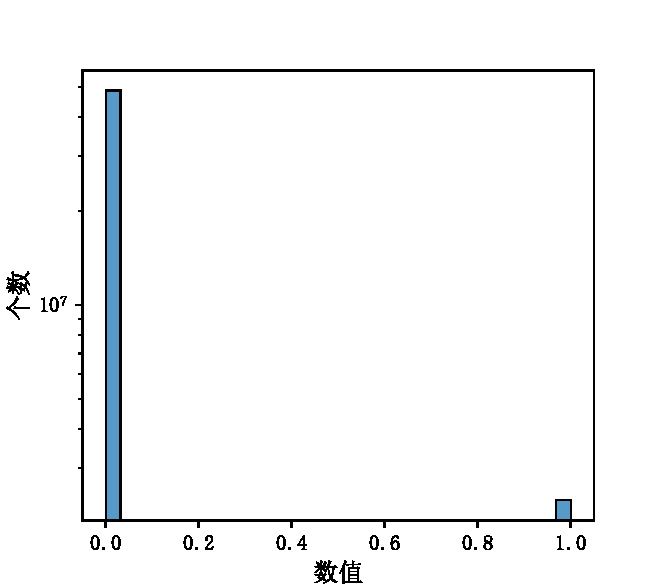
\includegraphics[width=1\linewidth]{img/preprocessing/cic2017_smalldata.pdf} % 插入SVG图片
\label{fig:cic2017_samllhist} % 子图的标签,用于交叉引用
\end{minipage}%
}
\subfloat[分布范围大的属性分布情况]{ % 插入第二个子图及其标题
\begin{minipage}{.5\textwidth}
\centering
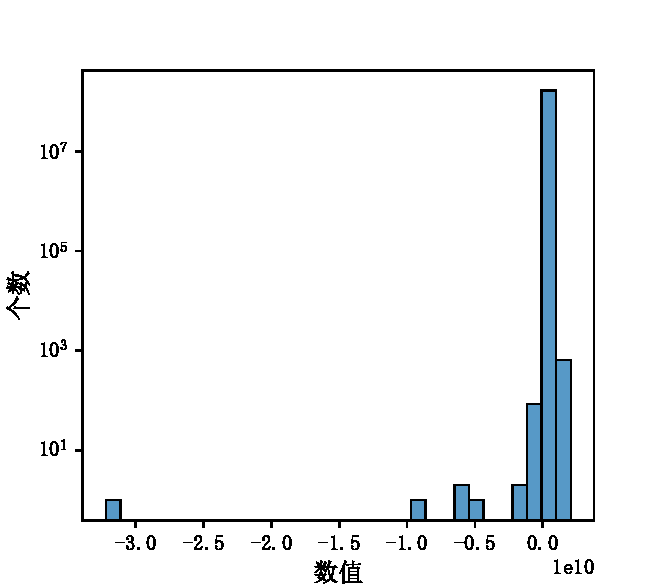
\includegraphics[width=1\linewidth]{img/preprocessing/cic2017_bigdata.pdf} % 插入SVG图片
\label{fig:cic2017_bighist}
\end{minipage}
}

\caption{CIC-IDS2017数据(正数部分)分布直方图} % 四张图片作为整体的标题
\label{fig:cic2017_hist}
\end{figure}

\section{数据预处理}
\subsection{数据清洗}
常见的数据集并不是规范的。

第一步是规范化整体数据,首先移除重复的列,然后查找数据中存在缺失数据的行,将这些行移除。

第二步是规范化数值类型,考虑到数据集中数值类型分布范围广,本章通过提出新的标准化算法,缩小数据分布范围,方便模型学习。

第三步是规范化非数值类型,对于非数值属性如协议类型,在不同数据集上可能是文本形式,也可能是协议代号形式,同一意义的不同格式数据会给模型学习带来困难,因此需要将其转为统一格式。


\subsection{数据转换}
\subsubsection{数值转换}

数据集中提供的数据包括均值、方差、包长度、字节数等。其中,一些数据,例如src\_bytes(从源主机到目标主机的数据字节数),其分布范围过大,不利于后续神经网络的处理。因此采用了以下算法\ref{alg:map_gt1},对分布范围大于1的属性值进行重新映射,以缩小分布范围。

映射前后数值分布情况如图\ref{fig:transf_hist}示。映射前分布不均,大部分数值分布在0附近,少部分数值较大,存在极少数负值,且负值分布极为稀疏。

映射后分布明显均匀,负数部分分布稀疏形况得到改善,正数部分分布更均匀,整体分布范围显著缩小,从十亿级别的分布变为-30至25之间,利于模型区分其中较小的数值差异。

\begin{figure}[htbp] % 创建一个新的figure环境
\centering % 居中对齐所有的子图

\subfloat[数据转换前分布情况]{ % 插入第一个子图及其标题
\begin{minipage}{.5\textwidth}
\centering % 居中对齐子图
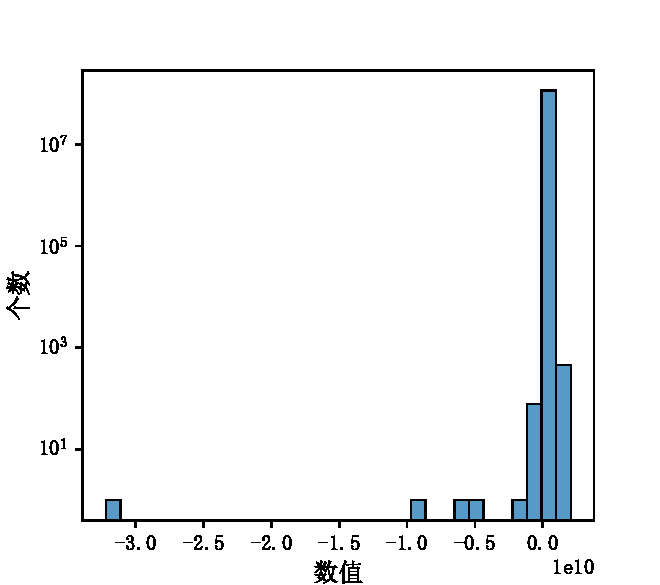
\includegraphics[width=1\linewidth]{img/preprocessing/logtransf_before.pdf} % 插入SVG图片
\label{fig:logtransf_before} % 子图的标签,用于交叉引用
\end{minipage}%
}
\subfloat[数据转换后分布情况]{ % 插入第二个子图及其标题
\begin{minipage}{.5\textwidth}
\centering
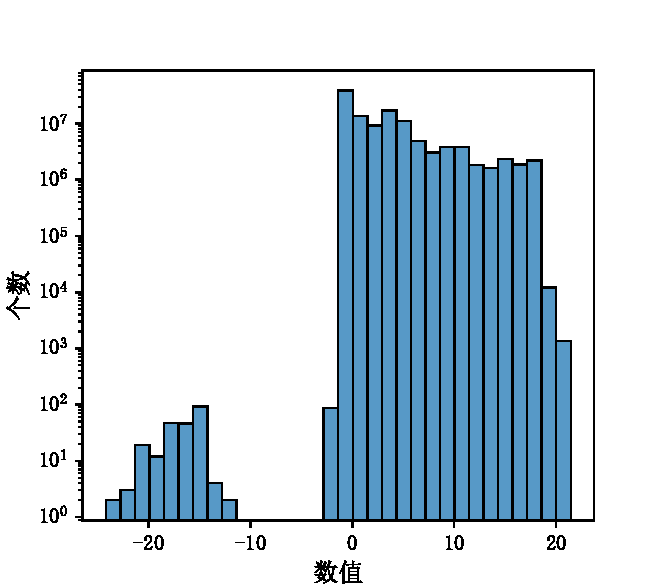
\includegraphics[width=1\linewidth]{img/preprocessing/logtransf_after.pdf} % 插入SVG图片
\label{fig:logtransf_after}
\end{minipage}
}

\caption{数值转换前后分布直方图} % 四张图片作为整体的标题
\label{fig:transf_hist}
\end{figure}

\begin{algorithm}[htbp]
\caption{数据预处理算法}
\begin{algorithmic}
\REQUIRE 矩阵 $A$
\ENSURE 处理后的矩阵 $B$
\STATE \textbf{步骤 1:} 对矩阵 $A$ 的每一列求绝对值的最大值
\FOR{每一列 $j$}
    \STATE $maxValue \gets 0$
    \FOR{每一行 $i$}
        \STATE $maxValue \gets \max(maxValue, |A_{i,j}|)$
    \ENDFOR
    \STATE $B_{*,j} \gets maxValue$
\ENDFOR
\STATE \textbf{步骤 2:} 筛选出最大值大于 1 的列
\STATE $selectedColumns \gets \emptyset$
\FOR{每一列 $j$}
    \IF{$B_{*,j} > 1$}
        \STATE $selectedColumns \gets selectedColumns \cup \{j\}$
    \ENDIF
\ENDFOR
\STATE \textbf{步骤 3:} 对筛选出的列,保留原符号,对其绝对值取对数
\FOR{每一列 $j \in selectedColumns$}
    \FOR{每一行 $i$}
        \STATE $B_{i,j} \gets \mathrm{sign}(A_{i,j}) \cdot \log(|A_{i,j}|)$
    \ENDFOR
\ENDFOR
\end{algorithmic}
\label{alg:map_gt1}
\end{algorithm}



\subsubsection{非数值转换}
本节定义的统一格式是文本形式。对于网络协议,会构建一个协议号至描述的映射表,从而将协议代号后转化为其对应的描述,过程如图\ref{fig:convert_ipport}示。

端口号的映射则较为复杂,一些网络服务有固定的端口号,但同一端口不同协议如TCP或UDP其对应的意义并不相同。因此需要构建二元组(端口号,协议)至描述的映射表,该映射表可准确地将端口号转化为其对应的描述,过程如图\ref{fig:convert_ipport}示。一般而言,服务器端的端口号是固定的,而客户端的端口号则不是固定的,因此需要将未进行映射的端口号描述置为“no available”,代表临时端口号。

\begin{figure}[htbp]
\centering % 居中对齐子图
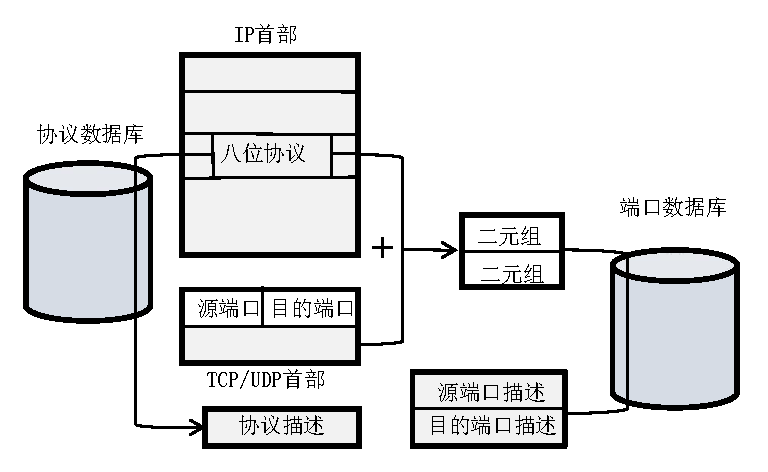
\includegraphics[width=1\linewidth]{img/preprocessing/convert_ipport.pdf} % 插入SVG图片
\caption{协议号与端口号转换过程}
\label{fig:convert_ipport} % 子图的标签,用于交叉引用
\end{figure}%

\subsection{数据切片与划分}
网络入侵检测数据集提供了连续的流量数据特征,模型无法处理过长的特征,因此需要将其进行切片。切片后需要对片段进行打乱,避免模型记忆序列本身而不是特征,同时还使不同类型的片段均匀分布。最后按比例将乱序片段划分为训练集与测试集,过程如图\ref{fig:divide_slice}示。

\begin{figure}[htbp]
\centering % 居中对齐子图
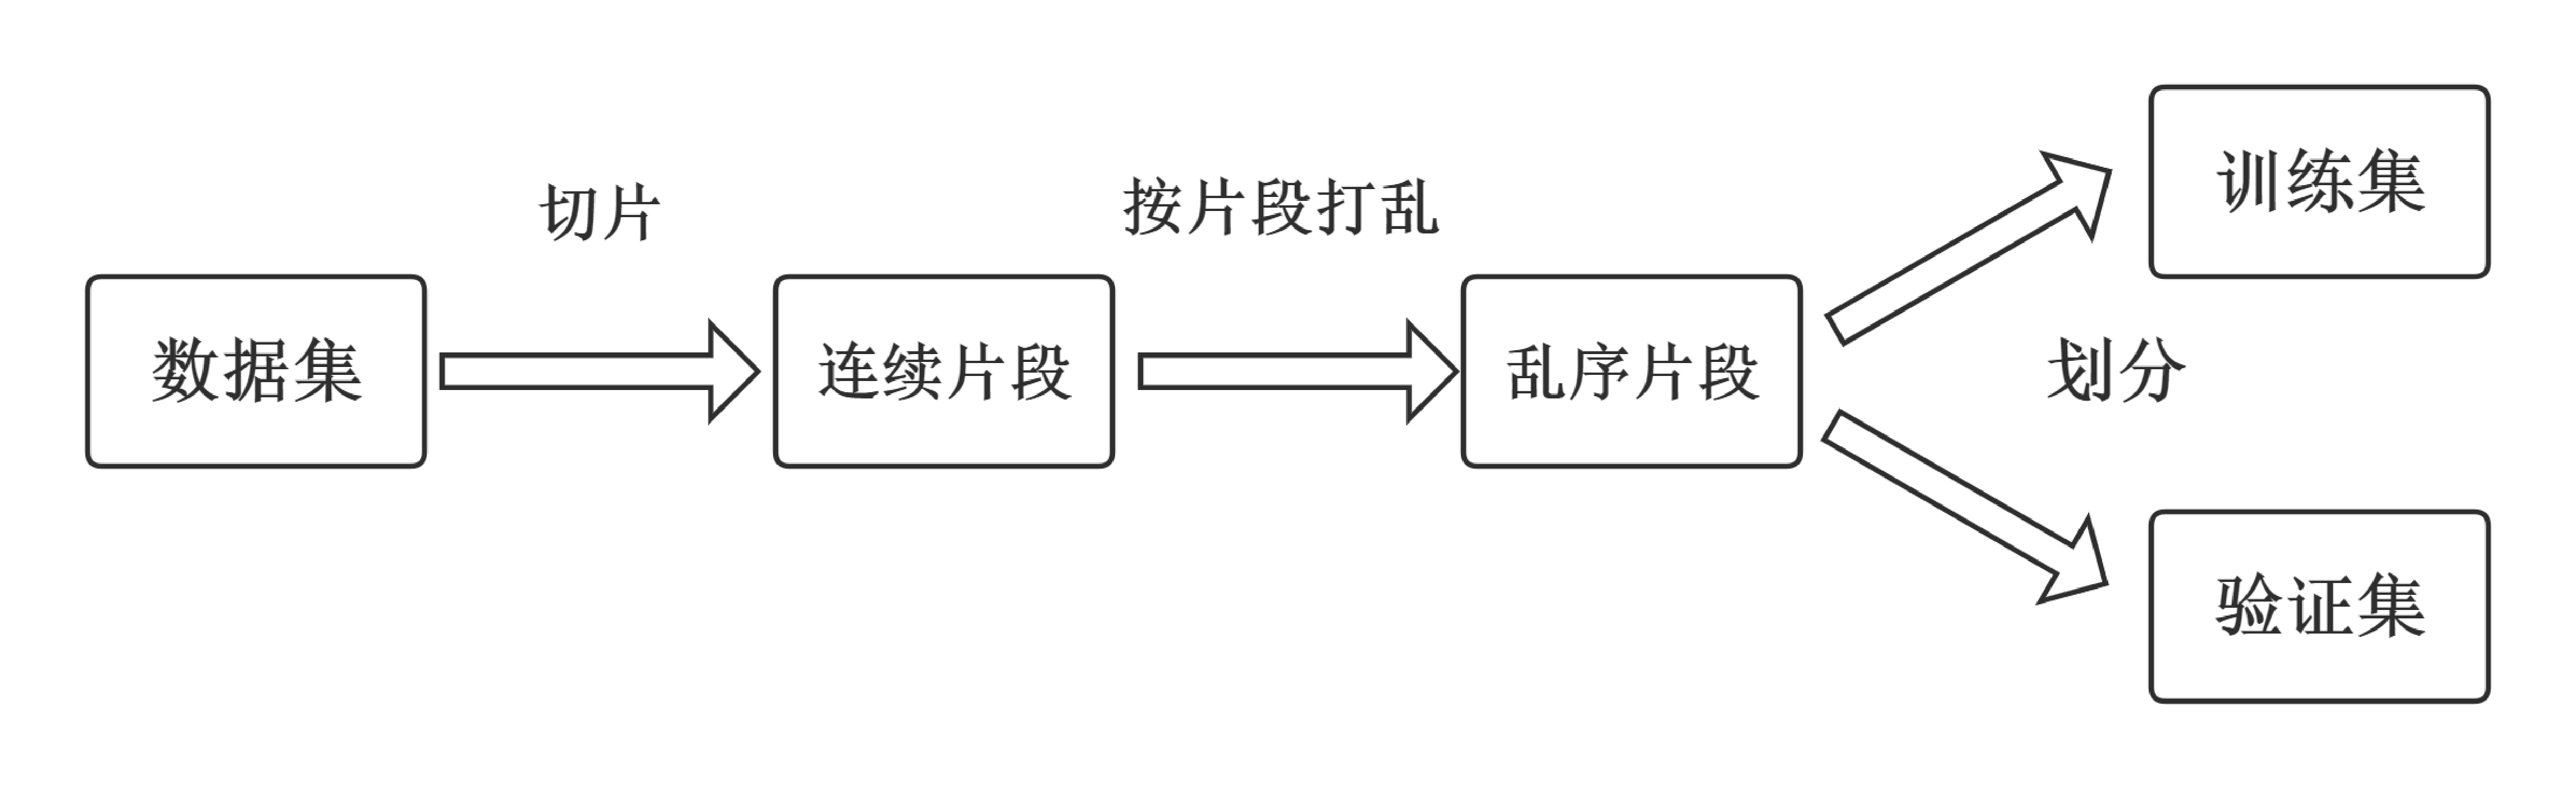
\includegraphics[width=1\linewidth]{img/preprocessing/divide_slice.pdf} % 插入SVG图片
\caption{数据集切片与划分过程}
\label{fig:divide_slice} % 子图的标签,用于交叉引用
\end{figure}%

\section{数据增强}
数据增强是机器学习中的常用技术,它通过数据集中已有样本合成新样本且新样本符合数据集中的数据分布。通过数据增强,扩充数据集大小,可以提高模型的泛化能力。若进行类别加权的数据增强,还可增加稀有样本出现频率以平衡数据集。

在上述处理过程中,为了实现时序建模,对数据集中连续的网络流量加窗,分割为长度相等的连接序列,该序列表示一段时间内网络连接情况。网络入侵检测中常见的数据增强方式是使用样本及其邻近样本重新合成新的数据,考虑到不同连接之间可能存在时间依赖关系,上述合成方式可能会破坏时间依赖关系,本章提出一种保持内部有序关系的序列数据增强算法\ref{algorithm:shuffle_data}。

\begin{algorithm}[htbp]
\caption{数据与固定标签的混洗算法}
\begin{algorithmic}
\REQUIRE 标签数组 $labels$
\ENSURE 根据标签混洗后的索引数组 $ans$,表示混洗后数组的新位置
\STATE \textbf{步骤 1:} 确定每个标签的索引位置
\STATE $unique\_labels, label\_positions \gets \mathrm{np.unique}(labels, \mathrm{return\_inverse=True})$
\STATE \textbf{步骤 2:} 为每个标签生成一个随机序列
\STATE $random\_label \gets \mathrm{np.random.permutation}(labels)$
\STATE \textbf{步骤 3:} 初始化一个与标签数组大小相同的索引数组
\STATE $shuffled\_indices \gets \mathrm{np.arange}(labels.size)$
\STATE $ans \gets shuffled\_indices.copy()$
\STATE \textbf{步骤 4:} 对于每个唯一标签,找到相应的数据索引并进行混洗
\FOR{每个标签 $label$ 在 $unique\_labels$ 中}
    \STATE $new\_mask \gets random\_label == label$
    \STATE $old\_mask \gets labels == label$
    \STATE $ans[new\_mask] \gets shuffled\_indices[old\_mask]$
\ENDFOR
\end{algorithmic}
\label{algorithm:shuffle_data}
\end{algorithm}


该算法的核心前提是不同类别之间的数据没有时间依赖。上述算法的核心在步骤四,普通混洗算法生成新元素的下标,本章提出的混洗算法则生成每个位置对应的类别。这一过程保证同一类别的数据虽然被映射到新位置,但其内部顺序仍然得以保持,从而维护了原数据中的时间依赖关系。

上述算法并没有直接生成新数据,而是生成增强后每个数据包的新位置。在保持时间依赖关系的情况下,增加数据多样性有助于提升模型的时序建模能力。


\section{本章小结}
本章主要介绍了所用的两种数据集,对每种数据集的特征进行分析。根据数据及特点进行了数据清洗、数值转换、数据切片过程,实现了数据的缩放,对网络流量中的非数值特征部分提出了一种新的转换方式,将先验知识(文本描述)引入其中,同时实现了不同数据集之间描述的统一化。提出了一种新的数据增强方法,利用标签,不改变数据分布的情况下,获得多样性的数据。


%%% Local Variables:
%%% mode: latex
%%% TeX-master: t
%%% End:

\chapter{基于多模态的入侵检测}
\label{cha:command}
本章节介绍如何使用Transformer在网络入侵领域进行多模态建模。Transformer最初被用于自然语言处理领域,由于其性能优越,因此被广泛应用于计算机视觉领域。随后人们发现了该架构在图像文本之间多模态建模能力。网络流量本身是一种模态,但对网络流量各种特征属性的描述以及其中的端口协议含义等属于另一种模态。数据集在给出数据的同时,会提供对该数据集的描述。对于传统的机器学习,该描述帮助研究者设计合理的数据预处理方法以及模型结构;对于深度学习模型,过去的研究者仅使用该描述确定预处理方法,特别是哪些属性应该被设置独热编码,以及确定模型的输入维度。

过去的研究都没有充分利用数据及描述信息,这主要是因为缺少合适的模型(Transformer)结构以及使用该结构进行多模态建模的正确方法(CLIP\cite{pmlr-v139-radford21a})。本章根据最新的研究进展,提出了一种多模态入侵检测模型,该模型将数据及描述信息融入分类过程中,实现文本辅助建模,并根据实验验证本章提出方法的有效性。

\section{相关技术介绍}
\subsection{Transformer模型介绍}
Transformer的出现在深度学习领域是变革性的,该模型在2017年被提出,作为性能卓越的自然语言处理的工具。该模型最大的特点在于其使用自注意力机制(Self-Attention)处理时序数据,这与之前主流的RNN或CNN模型截然不同。

使用自注意力机制进行建模,带来了以下优点:

\begin{enumerate}
    \item 自注意力机制能够捕获长距离相关信息且不会出现信息衰减,主流的RNN存在长距离信息衰减问题,CNN则只能建模局部信息。
    \item 自注意力机制并行处理序列信息,而RNN则是顺序处理,并行处理在一定程度上克服了访存限制对模型推理或训练速度的影响。
    \item 自注意力本质上是通过序列之间的相关性计算权重,即权重是动态的,而CNN等传统方法其权重值由模型本身决定是静态的。动态加权为模型提供了更高的灵活性和通用性。
\end{enumerate}

Transformer模型的结构由两部分组成:编码器以及解码器,如\ref{fig:transformer_struct}图示。

\begin{figure}[htbp]
    \centering
    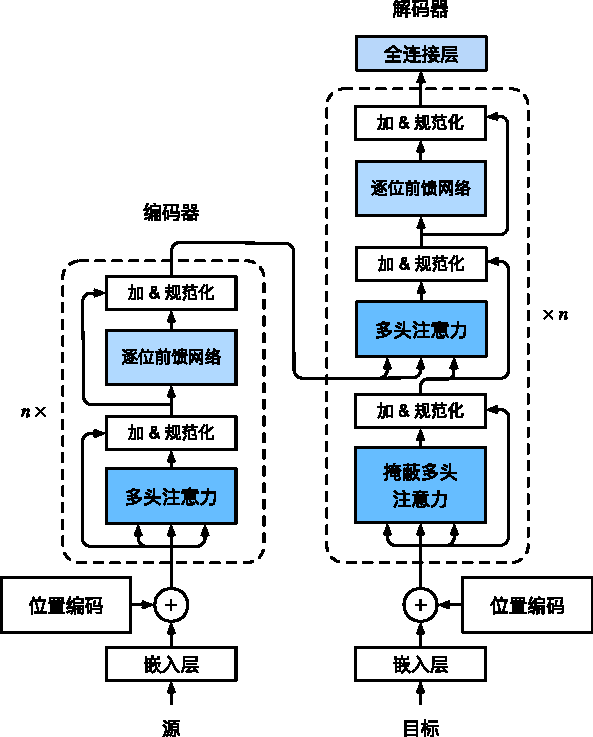
\includegraphics[width=.67\linewidth]{img/multimodal/transformer.pdf}
    \caption{Transformer架构\cite{zhang2023dive}}
    \label{fig:transformer_struct}
\end{figure}

左侧为编码器,编码器由多个相同的层组成,每一层中有两个子层,第一个子层是多头注意力,第二个子层是前馈网络。每个层在输出时都会进行层归一化以及残差连接。

右侧是解码器,同样由多层组成,每一层包含三个子层,增加的第三个子层用于接收编码器输入,在每一层的最下侧子层增加了掩码,用于保证信息由过去位置流向未来位置。

\subsection{BERT模型介绍}
BERT(Bidirectional Encoder Representations from Transformers),是一种基于Transformer架构的自然语言模型,关键特征在于双向,即在训练过程中同时考虑输入左侧以及右侧的全部上下文。传统的RNN只能进行单向建模,叠加两层不同方向的RNN才能实现双向建模。

BERT具有强大的自然语言理解能力,能感知句子中词语的深刻含义及不同词语之间的关系。该模型通过文本预训练进行学习,分别是掩码语言建模(Masked Language Modeling, MLM)和下一句预测(Next Sentence Prediction, NSP),前者遮挡词语并使用模型预测遮挡的内容,后者选取两句话,使用模型判断两句话是否存在上下文关系。经过预训练后,BERT只需在下游任务如句子情感分析等任务上进行微调即可取得较好性能。

对于每个输入序列,BERT模型都会将特殊的词语[CLS]对应的向量加入序列的开头。该向量在设计之初,用于捕捉整个输入序列的全局信息,在序列级别下游任务中该向量通常作为整个序列的特征。经典的序列集任务如句子情感分类,通常使用[CLS]作为输入,通过分类器得到最终分类结果。

\subsection{多模态模型介绍}
CLIP(Contrastive Language–Image Pre-training)是由OpenAI开发的多模态模型,其通过大量的图像-文本对进行训练,从而理解图像与自然语言之间的关系。其特点如下:
\begin{enumerate}
    \item 该模型通过对比学习进行训练,因此可完成多模态检索任务。通过文本检索图像,可在许多数据集上实现零样本图像分类。
    \item 该模型使用的文本编码器与图像编码器都基于Transformer架构,即通过同一架构的不同形式,可将文本与图像映射至同一特征空间中。
\end{enumerate}

CLIP由两部分组成,分别是图像编码器与文本编码器,如图\ref{fig:clip_struct}示。两者分别负责图像与文本的输入,并将其转化为统一空间中的向量表示。通过计算余弦相似度得到两向量之间的相似程度,在训练过程中是同一图像文本对之间的编码相互接近,而不同图像-文本对之间的编码相互远离。

\begin{figure}[htbp]
    \centering
    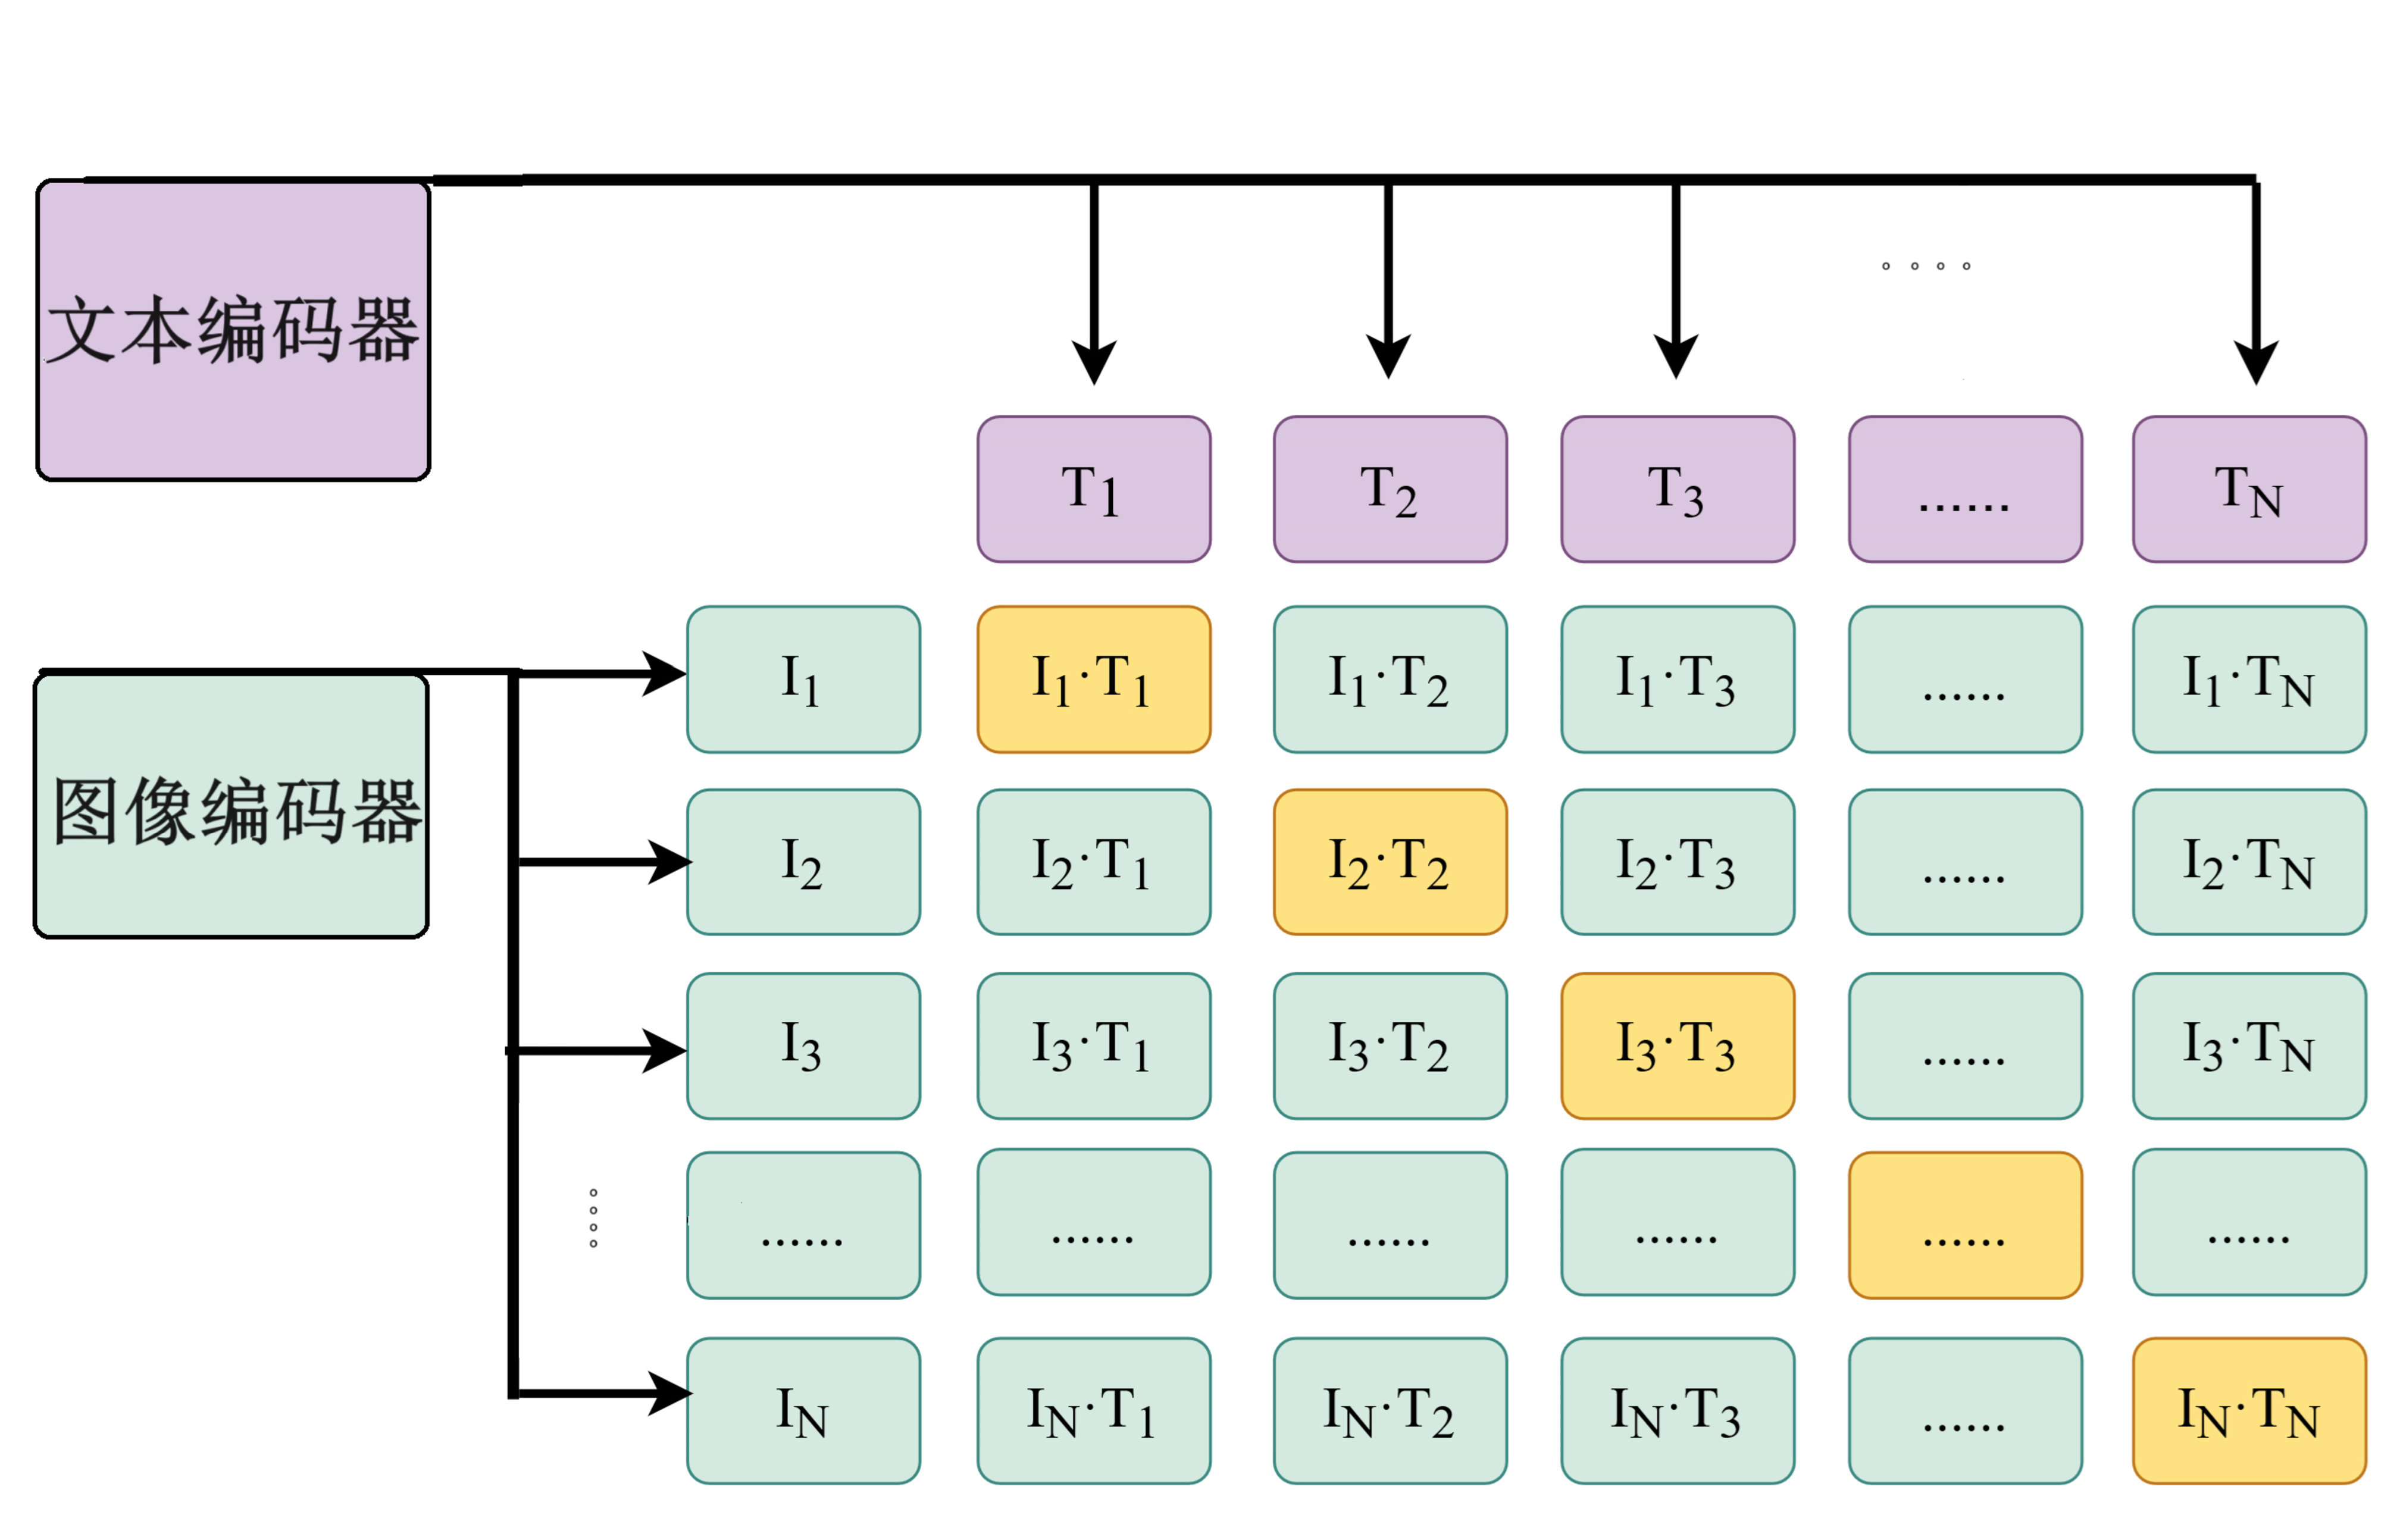
\includegraphics[width=1\linewidth]{img/multimodal/clip-overview.pdf}
    \caption{CLIP架构}
    \label{fig:clip_struct}
\end{figure}

CLIP模型的提出在多模态学习领域具有里程碑的意义,即通过大规模预训练模型可有效结合不同模态之间的信息,且两种编码器在本质上是同构的,Transformer架构在多模态学习中有极强的潜力。

\section{模型总体结构}

\begin{figure}[htbp]
    \centering
    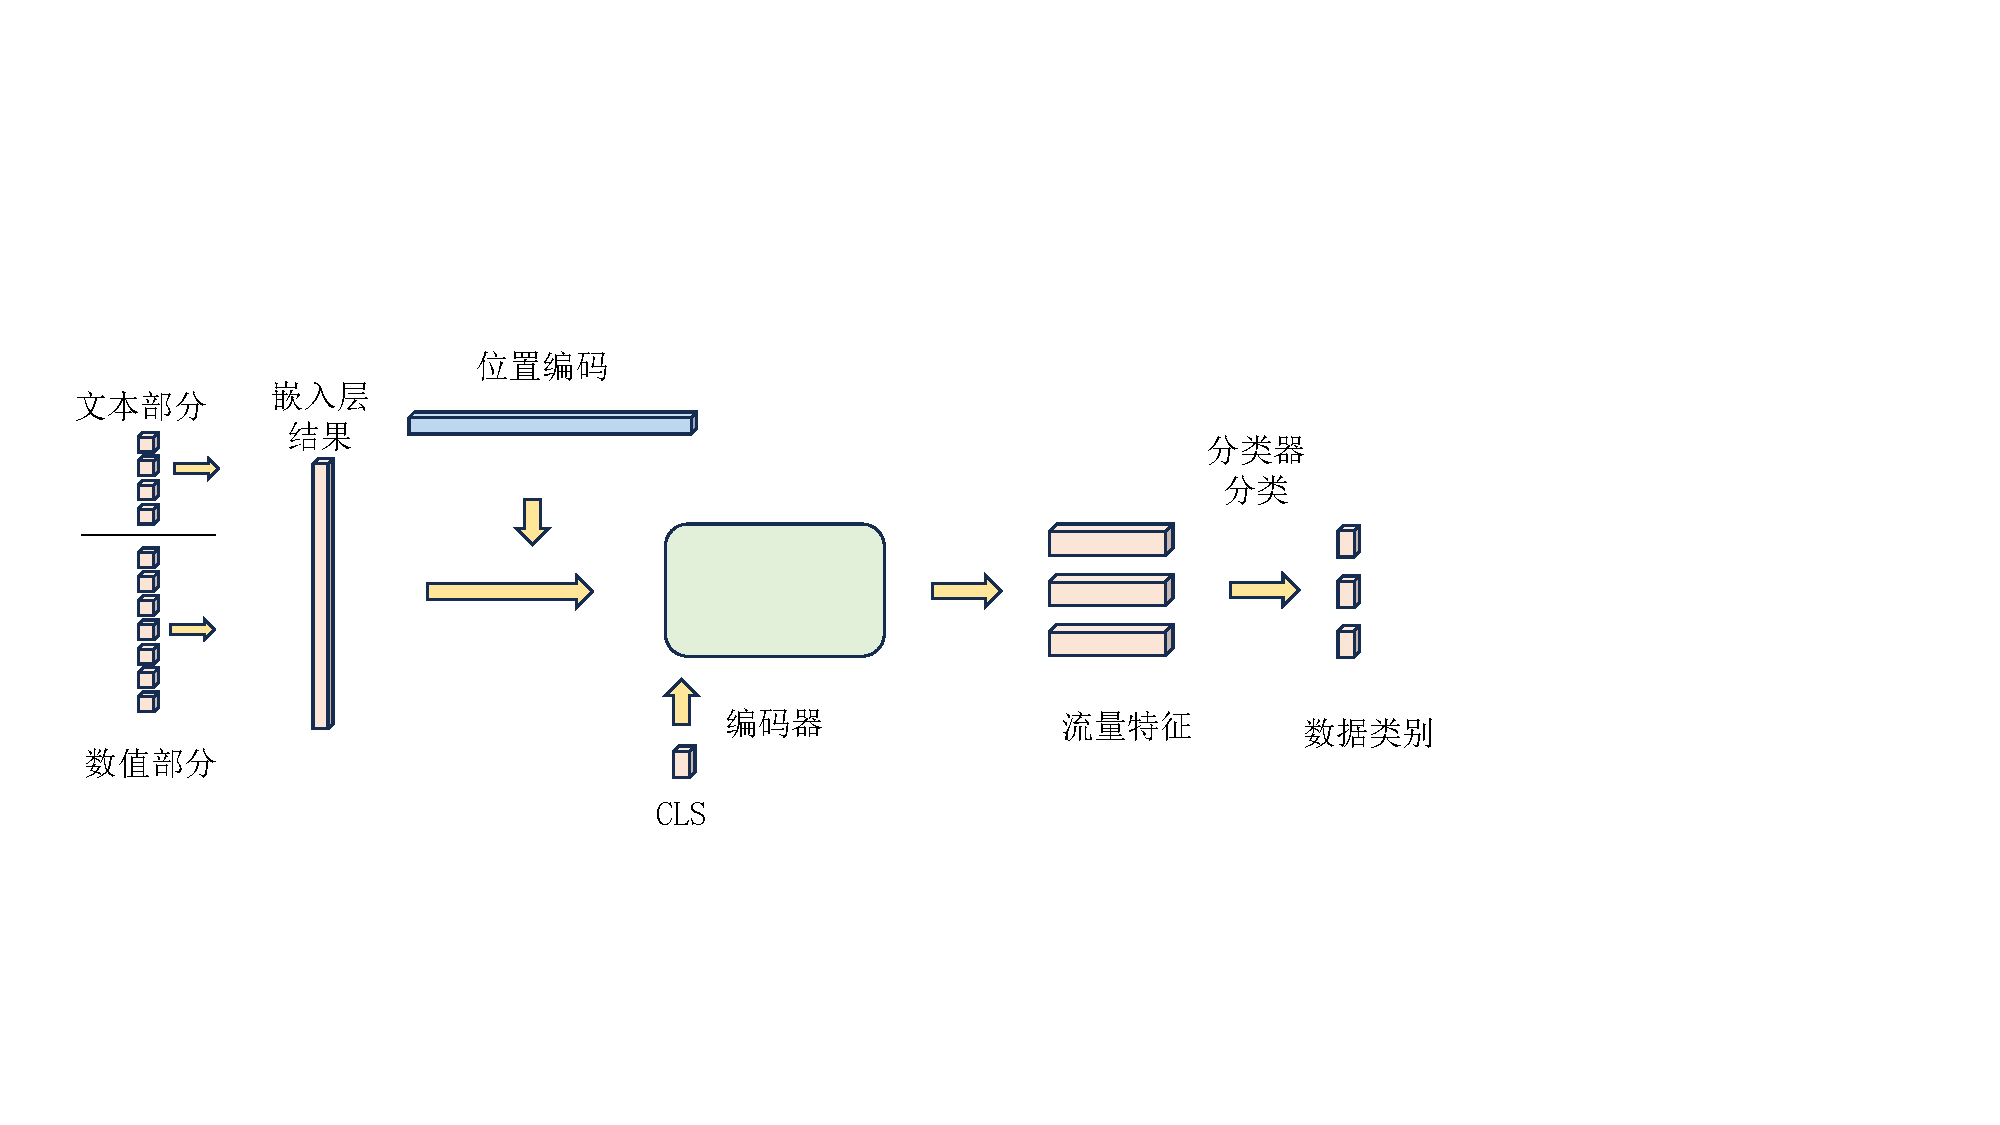
\includegraphics[width=1\linewidth]{img/multimodal/simple_overview.pdf}
    \caption{模型总体结构}
    \label{fig:simple_overview}
\end{figure}

本章提出的模型总体结构如图\ref{fig:simple_overview}示,其中左侧部分为语义辅助建模,是本章提出的多模态入侵检测模型的关键部分,其中包含新的数值嵌入方法、BERT加全连接层的文本嵌入方法以及数据集描述生成的位置编码。模型的输入是一个网络流量数据包的初步分析特征以及每个特征对应的文本描述。特征中包含多个属性,每个属性可以是数值类型或文本类型,若为文本则以索引形式给出。模型根据输入的特征判断数据包所属类别。模型由三个部分组成:嵌入层与位置编码、Transformer 编码器和分类器,Transformer 编码器由自注意力机制、归一化以及前馈神经网络组成。

在嵌入层,网络流量数据的初步分析特征 $\mathbf{X} = (\mathbf{x}_1, \mathbf{x}_2, \ldots, \mathbf{x}_n)$ 会进行变换以适应Transformer 编码器的输入特点。对于每个属性 $\mathbf{x}_i$,根据其模态分成两部分进行处理,最终得到128维的向量编码。在位置编码阶段,根据每个特征对应的文本描述生成位置编码。通过以上两个阶段,可得到了融合了属性值信息和属性描述信息的输入表示 $\mathbf{X}^{\mathrm{mm}} = (\mathbf{x}_1^{\mathrm{mm}}, \mathbf{x}_2^{\mathrm{mm}}, \ldots, \mathbf{x}_n^{\mathrm{mm}})$,其中
$$
\mathbf{x}_i^{\mathrm{mm}} = \mathbf{v}_i^{\mathrm{word}} + \mathbf{v}_i^{\mathrm{desc}}
$$
这里 $\mathbf{v}_i^{\mathrm{word}}$ 表示第 $i$ 个属性值的嵌入向量,可以是 $\mathbf{v}_i^{\mathrm{num}}$ 或 $\mathbf{v}_i^{\mathrm{text}}$。

随后将得到的输入表示 $\mathbf{X}^{\mathrm{mm}}$ 输入到4层的Transformer 编码器中。输入之前在序列的开头添加一个特殊的“[CLS]”标记,用于表示全局信息及整个数据包的特征,该标记的参数是可学习的。设第 $l$ 层Transformer Encoder的输出为 $\mathbf{Z}^{(l)} = (\mathbf{z}_0^{(l)}, \mathbf{z}_1^{(l)}, \ldots, \mathbf{z}_n^{(l)})$,其中 $\mathbf{z}_0^{(l)}$ 表示“[CLS]”标记对应的输出,$\mathbf{z}_i^{(l)}$ 表示第 $i$ 个属性的输出。最终得到第四层Transformer Encoder的“[CLS]”标记对应的输出,即输出的 $\mathbf{z}_0^{(4)}$ 作为整个数据包的表征向量。最后在分类阶段使用softmax函数将 $\mathbf{z}_0^{(4)}$映射到每个类别的概率。

\section{模型单层结构}

\subsection{语义辅助建模简介}
\begin{figure}[htbp]
    \centering
    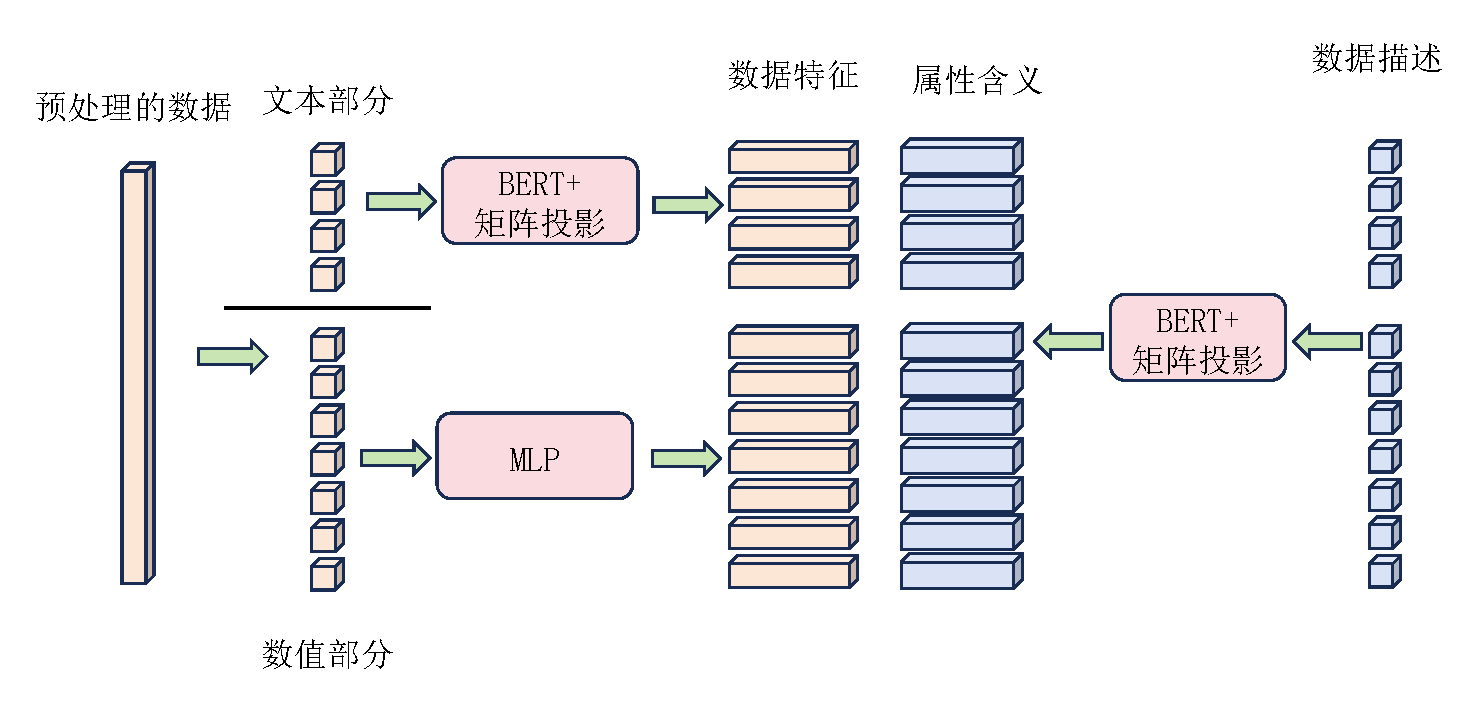
\includegraphics[width=\textwidth,height=\textheight,keepaspectratio]{img/multimodal/data2vec.pdf}
    \caption{获取嵌入向量及位置编码}
    \label{fig:data2vec}
\end{figure}

语义辅助建模包含两个过程数据嵌入以及位置编码,如图\ref{fig:data2vec}示,数据嵌入由两种嵌入方法组成,位置编码由数据集中对数据的描述文本生成,这两步是实现多模态模型的核心步骤。

嵌入层将输入数据转化为模型能处理的向量。嵌入的设计是多模态模型的关键部分,多模态模型必须处理与整合来自不同模态的信息,每种模态的格式各异。为有效融合来自各个模态的数据,对每种模态设计合适的向量嵌入方法,通过向量嵌入,不同模态的信息可在同一向量空间中表示。

Transformer核心特点是无状态,传统RNN在处理序列时会保留内部状态以跟踪序列的位置信息。Transformer感知位置关系的核心在于位置编码。对于多模态模型,位置编码的设计是核心,编码显式地提供了位置信息,位置信息可以是实际的前后关系,也可以是抽象位置(逻辑位置)如是否是文本以及是否是图像。序列中的每个元素加入位置编码后,除了包含其自身信息,还包含其所在位置信息。对于多模态模型,位置编码帮助模型识别元素的模态。

本章使用语言模型生成位置编码,为序列中每个元素提供灵活的位置信息;同时使用两种嵌入机制,将文本与数值均映射为128维向量。模型通过上述过程可有效分析来自文本与来自数值的信息,为单个流量生成更准确的向量描述。

总体过程如下:
输入序列 $ \mathbf{X} = (\mathbf{x}_1, \mathbf{x}_2, \ldots, \mathbf{x}_m) $中每个元素 $\mathbf{x}_i$ 是一个向量,向量的每个维度可能是数值或文字,总维度是$n$,与输入序列描述的个数相同。输入序列对应的描述 $ \mathbf{Desc} = (\mathbf{desc}_1, \mathbf{desc}_2, \ldots, \mathbf{desc}_n) $,对于序列中的每个元素 $\mathbf{x}_i$,执行以下步骤:

\begin{enumerate}
    \item 将 $\mathbf{x}_i$ 分离成数值部分 $\mathbf{n}_i$ 和文字部分 $\mathbf{t}_i$。
    \item 对数值部分 $\mathbf{n}_i$ 中的每个数值应用多层感知机 ${\mathrm{MLP}}_1$,得到数值的表征向量 $\mathbf{v}_i^{\mathrm{num}}$:
    \begin{equation}
    \mathbf{v}_i^{\mathrm{num}} = {\mathrm{MLP}}_1(\mathbf{n}_i)
    \end{equation}
    \item 使用BERT中获取文本部分 $\mathbf{t}_i$ 对应的句子表征向量 $\mathbf{w}_i$,然后应用线性投影 ${\mathrm{Proj}}_1$,得到文字的表征向量 $\mathbf{v}_i^{\mathrm{text}}$:
    \begin{equation}
    \mathbf{w}_i = {\mathrm{BERT}}(\mathbf{t}_i)
    \end{equation}
    \begin{equation}
    \mathbf{v}_i^{\mathrm{text}} = {\mathrm{Proj}}_1(\mathbf{w}_i)
    \end{equation}
    \item 对 $\mathbf{x}_i$ 向量中对应的描述$\mathbf{desc}_i$ ,从使用BERT获得对应的句子表征向量 $\mathbf{d}_i$,然后应用线性投影 ${\mathrm{Proj}}_2$,得到描述的表征向量 $\mathbf{v}_i^{\mathrm{desc}}$:
    \begin{equation}
    \mathbf{d}_i = {\mathrm{BERT}}(\mathbf{desc}_i)
    \end{equation}
    \begin{equation}
    \mathbf{v}_i^{\mathrm{desc}} = {\mathrm{Proj}}_2(\mathbf{d}_i)
    \end{equation}
    
\end{enumerate}

最终,对于每个元素 $\mathbf{x}_i$,可得数值表征向量 $\mathbf{v}_i^{\mathrm{num}}$或文字表征向量 $\mathbf{v}_i^{\mathrm{text}}$,以及用于位置编码的描述表征向量 $\mathbf{v}_i^{\mathrm{desc}}$。对于前两种表征向量,按照其位置统称为 $\mathbf{v}_i^{\mathrm{word}}$。

经过语言辅助建模后输入序列 $ \mathbf{X}$变为了$ \mathbf{X}^{\mathrm{mm}} = (\mathbf{x}_1^{\mathrm{mm}}, \mathbf{x}_2^{\mathrm{mm}}, \ldots, \mathbf{x}_n^{\mathrm{mm}}) $,其中${x}_i^{\mathrm{mm}}$由以下方式得到:
    \begin{equation}
    \mathbf{x}_i^{\mathrm{mm}} = \mathbf{v}_i^{\mathrm{word}} + \mathbf{v}_i^{\mathrm{desc}}
    \end{equation}
   
后续只要将这些输入传统的Transformer模型,就可以实现对网络流量的建模。经过若干层变换后提取[CLS]即可得到固定维度为$d$的特征,该特征理论上与数据集无关,与流量本身的特点有关。

\subsection{嵌入层}
基于Transformer架构的模型在输入的第一步进行数据嵌入,该过程对数据进行处理,将信息转化为描述其含义的向量,方便模型对数据进行分析与特征提取。

面向自然语言处理的模型常采用的方法是词向量嵌入,即首先从文本数据中识别唯一单词建立词表,随后为每个词分配一个向量,每次都会根据查表结果替换为对应的向量,该向量会在随后的训练过程中进行调整。使用词向量可使在语义上含义相近的词在高倍空间其相对距离更近,因此词向量可有效表达每个词的复杂含义。与稀疏的独热编码相比,词向量是密集的,可有效节约存储空间。

面向计算机视觉的模型常采用的方法是图像切块,每个图像小块再进行线性映射或其他形式映射后,其表现形式与进行了词向量线路的单词相同,可进入Transformer架构中。

流量特征中包含许多文本信息如协议描述、所用端口的描述,这些文本已在数据处理过程中构建嵌入向量表并转化为索引值。传统方法将文本转换为独热编码,但这种方式会损失一部分文字的含义,且对端口号进行转换时,会生成非常稀疏的向量,不利于模型学习。

为了充分地体现文本之间的细微差异,重编码部分使用预训练BERT模型生成文本特征向量,从而得到文字对应的编码。具体方法是取[CLS]作为文本的向量表征。

理想情况下,将BERT嵌入到模型中并随着模型进行微调是最佳做法。然而,由于BERT的计算量较大,直接使用可能导致模型运行缓慢,无法实时监测流量情况。因此可将BERT视为参数固定的特征提取器,采用预计算加快模型计算速度。在数据预处理阶段,已经构建了句表,此表中包含可能用到的句子,预计算需要在模型初始化阶段,通过预训练的BERT系列中的“bert-large”生成句子对应的表征向量(维度1024)填充到句表中。在训练和推理阶段,模型可以直接使用处理后的特征结果,而无需运行完整的BERT模型。此方法既提高了效率,又能有效保留文字的语义信息。

以上过程可得到预计算的句子表征向量,所用的特征提取器BERT内部参数被冻结,即提取的嵌入向量表(句表)中向量并不会根据下游任务进行调整,为了针对网络入侵检测中的描述特征提取任务进行优化,需要为其增加可学习参数。另一方面,BERT得到的向量维度较高,对网络流量特征描述的句子较为简单,高维度向量中包含较多冗余,且影响计算速度。

因此需要引入参数可调节的矩阵进行投影,将句子表征向量从适应预训练任务的输出空间映射至适应入侵检测任务的空间。同时进行降维,以帮助模型适应流量检测的实时性要求。本节使用输入维度为1024,输出维度为128的线性变换进行投影,预计算后得到的嵌入向量表(句表)中的向量映射至合适的输出空间。

该设计可以把BERT模型和后面的投影看作整体,即规模较大且可以微调的语言模型。通常微调需要将数据经过BERT和线性投影变换进行前向传播,然后再反向传播经过线性投影变换,其中绝大多数计算量由BERT产生。

考虑到实际输入的文本是有限的,上述预计算过程已对可能输入的文本进行特征提取,因此可以将前向传播的第一步变为一种查表过程。此时微调就变成了查表过程加矩阵乘法的前向和反向传播过程,微调过程中矩阵投影的权重可在训练过程中调整,模型在较低计算量的情况下,仍保持学习能力。

Transformer输入序列的每一个向量维度都是相等的,此处输入序列的每一个元素指流量特征的每一个属性。网络流量特征中,大部分属性为数值类型,因此需将数值映射为句子表征向量,即将1024维数值映射为128维。此处使用简单的MLP实现数值映射,输入维度为1,隐藏层为512,输出维度为128,激活函数使用ReLU,引入该函数可增强模型非线性表示能力。此处MLP的隐藏层与输出维度参照Transformer中MLP进行设计,隐藏层与输出维度之比为2:1。

网络流量特征经过上述两个过程,每个属性值都转化为维度相同的向量。
\subsection{位置编码}
位置编码是Transformer架构的重要组成部分。在传统RNN模型,模型以递归方式按顺序处理输入序列,输入过程本身已包含位置信息。Transformer并行处理输入序列,序列中每个向量在形式上等价,若不进行位置编码,则模型无法区分向量在序列中的顺序。

Transformer架构解决这一问题的方法是引入位置编码。位置编码为模型提供显式的顺序信息,其具体方法是将与位置有关的向量添加到输入序列的每个元素中。原始Transformer使用余弦编码。

余弦位置编码基于三角函数构建,位置编码由定义好的函数计算得出,而不是模型在学习过程中得到。序列各处的位置编码维度与嵌入后的向量维度相同,但内容并不相同。对于位置 $pos$ 以及维度 $i$,在序列中位置编码 $\mathbf{PE}_{(pos, i)}$ 由公式\ref{eq:pe_cosine}定义。

\begin{equation}
\begin{aligned}
\mathbf{PE}_{(pos, 2i)} &= \sin\left(\frac{pos}{10000^{\frac{2i}{d}}}\right) \\
\mathbf{PE}_{(pos, 2i+1)} &= \cos\left(\frac{pos}{10000^{\frac{2i}{d}}}\right) \\
\end{aligned}
\label{eq:pe_cosine}
\end{equation}

其中 $pos$ 是序列中的位置,$i$ 是维度下标, $d$ 是信息编码后的维度。除固定的位置编码外,模型可在学习过程中调整位置编码,这被称为可学习位置编码。

可学习位置编码是模型用来学习序列中位置信息的一种参数。与预定义的余弦位置编码不同,可学习位置编码是模型参数的一部分,在模型训练中通过梯度下降进行调整。可学习位置编码 $\mathbf{E}_{pos}$ 由公式\ref{eq:Epos}定义。

\begin{equation}
\label{eq:Epos}
\mathbf{E}_{pos} = \{\mathbf{e}_{1}, \mathbf{e}_{2}, \ldots, \mathbf{e}_{N}\}
\end{equation}


其中 $N$ 是序列中的最大长度, $\mathbf{e}_{i}$ 是序列中第 $i$ 个位置的可学习位置编码。

在训练过程中模型会调整 $e_{i}$ 以最小化损失函数,虽然其长度相比余弦位置编码有一定限制,但其对特定任务的适应性更好。

在本章提出的模型中,位置编码需要对流量特征的每个属性提供信息。此位置的特点是,位置与其在输入序列中的相对位置并没有关系,而是与其对应的描述有关。通常情况下各位置的描述是固定的,因此可使用上述两种编码为模型提供属性描述信息。这种编码缺少灵活性,若新数据集中属性增加或删减,原有的位置编码可能会失效。

为解决上述两种编码在网络入侵检测任务上的局限性,本节提出一种新的语义辅助位置编码。该编码保持灵活性且通过引入语义信息实现对流量特征的更准确提取。与常规位置编码不同,此处的语义辅助位置编码并不是指的向量中每个元素在序列中的排列位置,而指的是每一个元素所对应的含义。此含义由数据集的每一列标题给出。

数据集的描述中会对每一列进行具体的介绍,说明其含义以及取值范围。因此可以使用预训练语言模型,如BERT,根据介绍文本生成每一列位置编码,其中包含每一列的含义。
BERT输入向量的维度较高,且原输出向量仅适合预训练任务,并不适合位置编码任务,位置编码相比之前的文本嵌入句子多样性更少,高维度向量会引入冗余信息,同样需要进行调整以实现降维处理。本节使用可学习的投影矩阵实现这一目的,使用投影矩阵将BERT生成的列标题描述向量转投影至适合位置编码的向量空间。

对于每个标题描述对应的[CLS]使用一个输入维度为1024,输出维度为128的矩阵变换实现,该矩阵是可学习的。经过变换,标题描述向量被映射到新空间。在此过程中BERT作为参数固定的特征提取器,[CLS]通过预计算得出,因此每次计算位置编码都只需对每个标题描述向量进行矩阵投影即可。这使模型能在实时计算的同时,有效利用数据集中对每一列的描述信息建立位置编码,以便模型对流量进行更精确建模。上述过程保持了模型的通用性,当数据集的格式发生变化,只需重新配置每一列的描述文本,再使用BERT进行一次推理,即可得到新的位置编码,不需要重新训练生成。

\subsection{自注意力机制}
自注意力机制是Transformer模型最大的特点,该过程本质上实现了对数据的自适应加权,过程可分为三个阶段。

第一步,使用三个投影矩阵$\mathbf{W}^{\mathrm{Q}} ,\mathbf{W}^{\mathrm{K}},\mathbf{W}^{\mathrm{V}}$,对经过语义辅助建模的$ \mathbf{X}^{\mathrm{mm}}$进行线性变换,可得到输入对应的查询、键和值矩阵:
\begin{equation}
\mathbf{Q} = \mathbf{X}\mathbf{W}^{\mathrm{Q}}, \quad \mathbf{K} = \mathbf{X}\mathbf{W}^{\mathrm{K}}, \quad \mathbf{V} = \mathbf{X}\mathbf{W}^{\mathrm{V}}
\end{equation}
如图\ref{fig:attention_proj} 示,该过程将输入序列转化为三个维度相同序列,这三个序列分别被称为查询、键、值。生成三种不同的序列可帮助模型对不同位置元素之间的相关性进行建模,建模过程类似信息检索,三个序列的含义如下:
\begin{itemize}
    \item 查询(Q)代表当前元素对序列中其他元素的关注程度,在计算注意力时,主要用于与其他元素的键进行比较,以确定相关性的强度。
    \item 键(K)代表序列的特征,该特征用于匹配查询。在计算注意力时,该元素决定了对查询来源的影响程度。
    \item 值(V)包含每个元素的实际信息。该元素根据Q与K之间的相关性被加权,权重反映了序列中全部元素对当前元素的重要程度。
\end{itemize}

\begin{figure}[htbp]
    \centering
    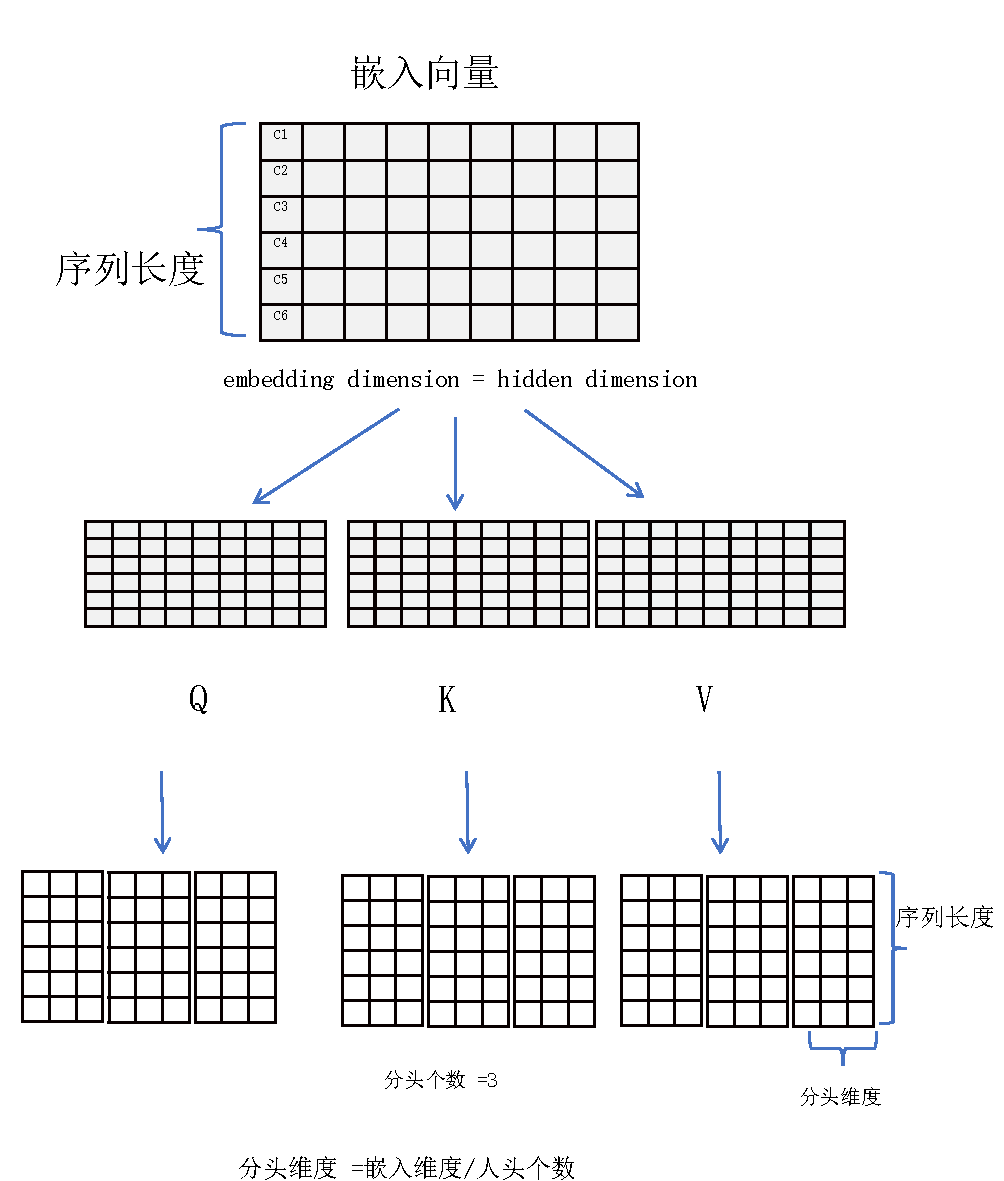
\includegraphics[width=0.85\linewidth]{img/multimodal/attention_proj.pdf}
    \caption{查询(Query)、键(Key)、值(Value)的生成}
    \label{fig:attention_proj}
\end{figure}

序列被划分为三个序列后,每个序列会被分成$h$个头,每个头对应的维度是${embedding\_dimension}/{h}$,此过程要求输入序列的维度必须被$h$整除。通过引入多个头,每个头都可以独立学到不同的注意力,即可以关注序列中的不同部分,而不是关注全局相关性,有助于模型捕捉更丰富的序列依赖关系。

每个头都可以独立计算注意力分数$\mathbf{Attention\_score}$,其中一个头的注意力计算分数如图\ref{fig:attention_softmax}示,将$\mathbf{Q}$与$\mathbf{K}$进行矩阵乘法,即对$\mathbf{Q}$的每一行以及$\mathbf{K}$的每一列计算向量点积,点积表示两个向量的相似程度,右侧注意力矩阵中第i行第j列的含义是第i个字与第j个字在该头的注意力值。对于两个服从均值为0,方差为1的正态分布的向量进行点积,点积后的结果就是向量的维度大小。因此在计算注意力分数时,需要在点积后,进行缩放,除以$\sqrt{d}$  ,将方差调整为1,避免高维度向量计算得出大数值,而导致梯度消失或爆炸。最后为保证某一元素对其他所有元素的注意力分数权值和为1,需要对最终的注意力分数按图\ref{fig:attention_softmax}中的行方向计算softmax。
\begin{figure}[htbp]
    \centering
    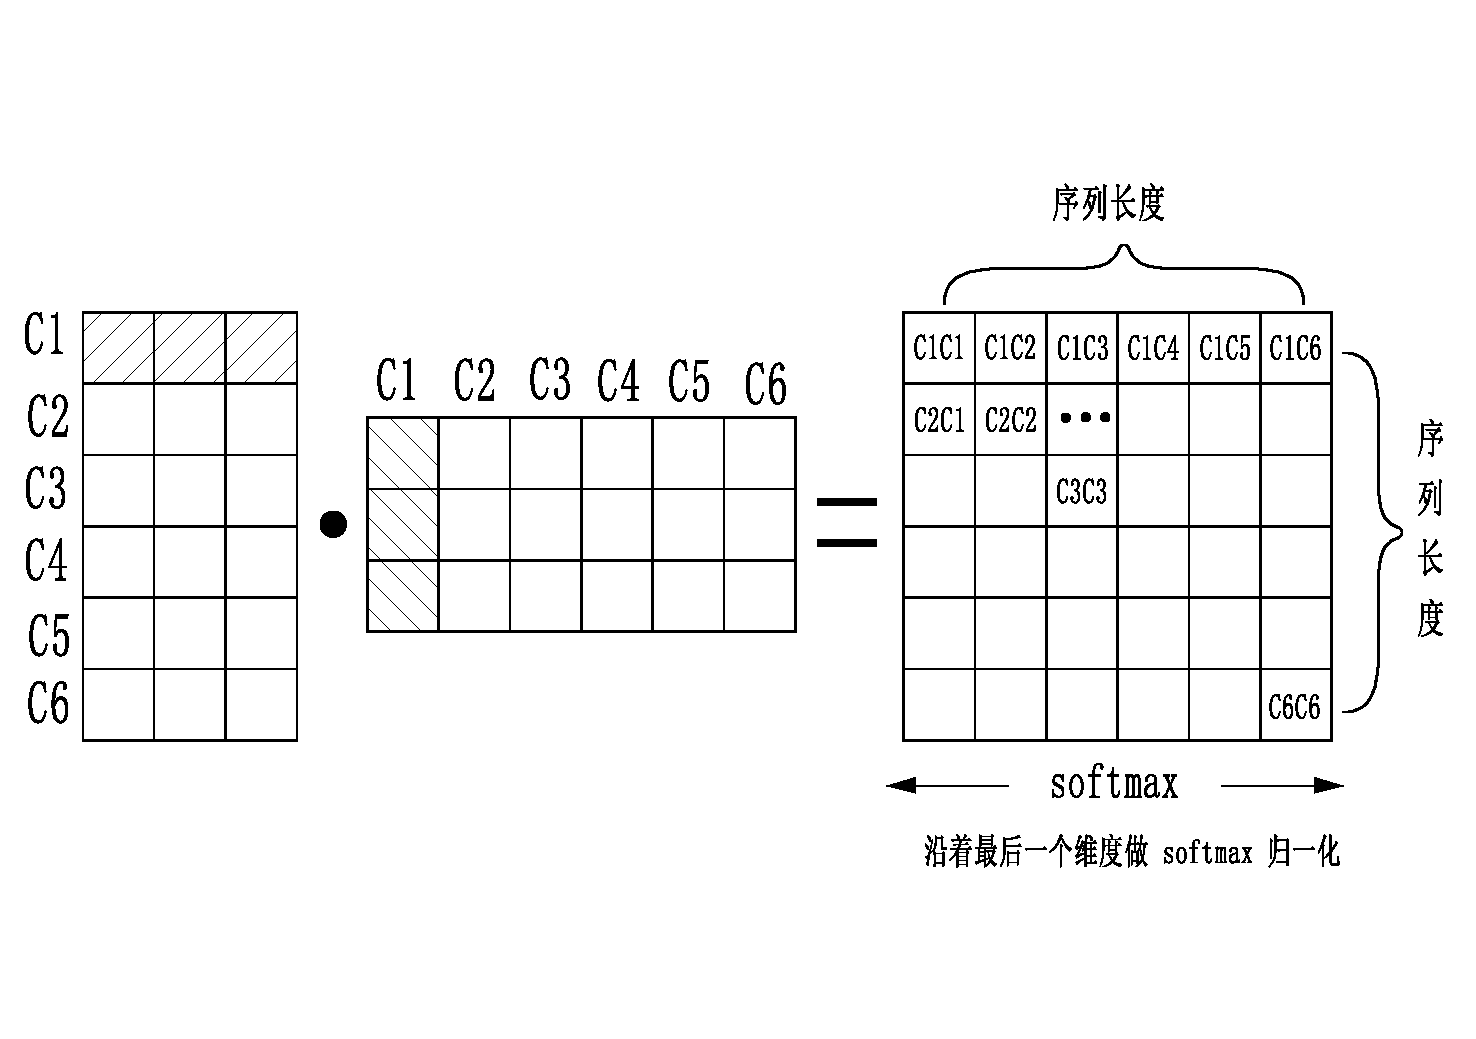
\includegraphics[width=0.8\linewidth]{img/multimodal/attention_softmax.pdf}
    \caption{注意力分数的计算 }
    \label{fig:attention_softmax}
\end{figure}
\begin{equation}
{\mathbf{Attention\_score}} = {\mathrm{softmax}}\left(\frac{\mathbf{Q}\mathbf{K}^{\mathrm{T}}}{\sqrt{d}}\right)
\end{equation}


最后在加权阶段,取每个头的注意力矩阵以及对应头的V,进行矩阵乘法如图\ref{fig:attention_fin}示。使用注意力权重对V进行加权,最终每个元素的值都包含了来自其他位置元素的信息。

\begin{equation}
{\mathbf{Attention}}=\mathbf{Attention\_score} \times \mathbf{V}= {\mathrm{softmax}}\left(\frac{\mathbf{Q}\mathbf{K}^T}{\sqrt{d}}\right)\mathbf{V}
\end{equation}

\begin{figure}
    \centering
    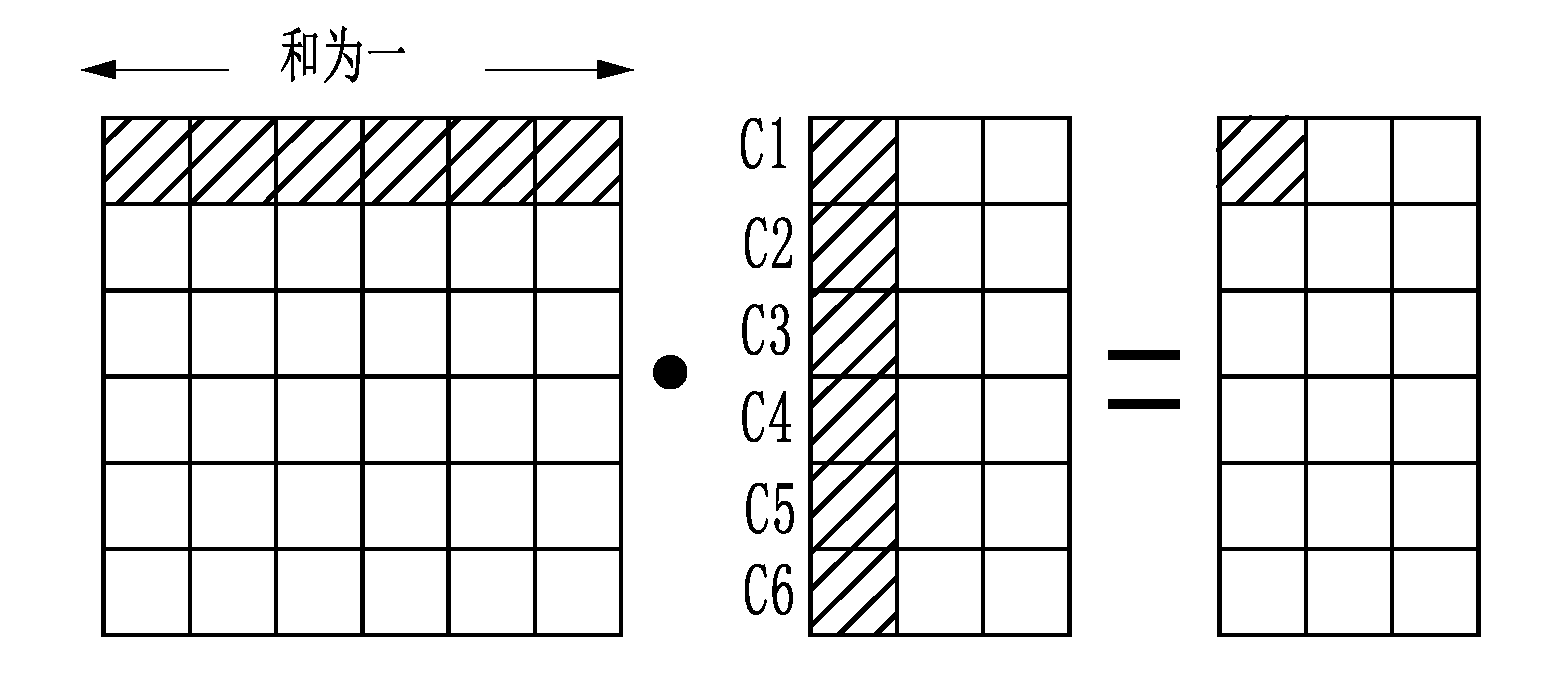
\includegraphics[width=0.8\linewidth]{img/multimodal/attention_fin.pdf}
    \caption{加权值向量的组合并生成输出 }
    \label{fig:attention_fin}
\end{figure}

\subsection{归一化}

在批次训练时有样本批次 $\mathbf{X} \in \mathbb{R}^{N \times D}$ ,其中 $N$ 是批次中样本的个数, $D$ 是隐藏层维度,对一个样本 $\mathbf{x} \in \mathbb{R}^D$, 可以计算均值 $\mu$ 以及方差 $\sigma^2$:

\begin{equation}
\mu = \frac{1}{D} \sum_{i=1}^{D} \mathbf{x}_i
\end{equation}

\begin{equation}
\sigma^2 = \frac{1}{D} \sum_{i=1}^{D} (\mathbf{x}_i - \mu)^2
\end{equation}


可以对输入每一个 $\mathbf{x}$ 归一化后的结果$\hat{\mathbf{x}}_i$:

\begin{equation}
\hat{\mathbf{x}}_i = \frac{\mathbf{x}_i - \mu}{\sqrt{\sigma^2 + \epsilon}}
\end{equation}

其中 $\epsilon$ 是一个小常量,用于避免除零错误。 然后归一化的 $\hat{x}$ 会被重新设置均值与方差以获得层归一化后的 $y$:

\begin{equation}
\mathbf{y}_i = \gamma \hat{\mathbf{x}}_i + \beta
\end{equation}

其中 $\gamma$ 和 $\beta$ 为输出需要被设置的方差与均值,这两个值均可随模型训练进行调整,因此模型可自适应调整每一层的输出分布,从而具有更灵活的特征提取能力。

\subsection{前馈神经网络}
Transformer 的前馈神经网络通常由MLP构成,其主要作用是增强模型的非线性表达能力。自注意力机制中都是线性变换,而前馈神经网络引入了非线性的激活函数,使模型能学到输入数据中的复杂关系,增强了模型对于信息的理解能力。该网络的作用是将自注意力机制生成的输出转化为新的特征表示。本章中使用的前馈神经网络结构如下:
\begin{equation}
\mathrm{FFN}(\mathbf{x})=\max(0, \mathbf{b_1} + \mathbf{W_1}\mathbf{x}) \mathbf{W_2} + \mathbf{b_2}
\end{equation}
其中$\mathbf{x}$是输入序列,$W_1\in \mathbb{R}^{d \times 2d}$和$W_2\in \mathbb{R}^{2d \times d}$是可学习的权重映射矩阵,$b_1 \in \mathbb{R}^{2d}$和$b_2\in \mathbb{R}^{d}$是偏置向量。
其过程有三步:
\begin{itemize}
\item 将输入值使用矩阵变换并加上偏置,该输入值被映射至两倍维度向量空间。
\item 对映射后的值,使用ReLU函数进行激活,即对映射后的向量,将负数部分置为0。
\item 将激活后的值使用矩阵变换并加上偏置,激活值被映射为与输入维度相同的向量空间。
\end{itemize}

\subsection{分类器}
模型的最后一步是进行分类。传统的分类方法是添加一个全连接层,通过线性映射得到各个类别对应的权重向量,即:

\begin{equation}
\mathbf{z} = \mathbf{W}\mathbf{x} + \mathbf{b}
\end{equation}

其中,$\mathbf{W}$ 是权重矩阵,$\mathbf{x}$ 是输入特征向量,$\mathbf{b}$ 是偏置向量。接着,通过计算softmax函数可以得到每个类别对应的概率:

\begin{equation}
P(\mathbf{y}_i|\mathbf{x}) = \frac{e^{\mathbf{z}_i}}{\sum_j e^{\mathbf{z}_j}} 
\end{equation}

\section{模型训练}

\subsection{损失函数}
损失函数用于评估模型性能,本章中使用的交叉熵损失函数评价模型的输出值与样本实际标签之间的差距大小,该函数在多分类问题中定义为:

\begin{equation}
L(\mathbf{y}, \mathbf{\hat{y}}) = -\sum_{c=1}^M y_{o,c} \log(\hat{y}_{o,c})
\end{equation}
其中 $M$ 是类别的总数,$y_{o,c}$ 是二进制指示器(0或1),表示类别 $c$ 是否是观察 $o$ 的正确分类,$\hat{y}_{o,c}$ 是模型预测观察 $o$ 为类别 $c$ 的概率。

入侵检测数据集呈现极度不均衡,为了解决这一问题可引入权重向量 $\mathbf{w}$,其中 $w_c$ 是与类别 $c$ 相关联的权重。改进后的加权交叉熵损失函数可以写为:

\begin{equation}
L(\mathbf{y}, \mathbf{\hat{y}}, \mathbf{w}) = -\sum_{c=1}^M w_c \cdot y_{o,c} \log(\hat{y}_{o,c})
\end{equation}
权重 $w_c$ 可以根据类别 $c$ 的样本频率来设置。为少样本类别设置更高的权重,可实现数据集的平衡,本章中各类别权重值为各类别频率的平方根倒数归一化后的结果。

模型对小样本类别误判后会得到更大程度调整使模型更注重该类别,从而减少模型在训练过程中对多数类别的偏好,最终在全部类别上都能有较高的分类准确率。

\subsection{优化器}
优化器调整模型参数,最小化损失函数,使模型预测更准确。本章使用AdamW优化器,为Adam(Adaptive Moment Estimation)的改进形式。Adam更新过程如下:

% 参数更新规则
\begin{equation}
\begin{aligned}
m_t &= \beta_1 \cdot m_{t-1} + (1 - \beta_1) \cdot g_t, \\
v_t &= \beta_2 \cdot v_{t-1} + (1 - \beta_2) \cdot g_t^2, \\
\hat{m}_t &= \frac{m_t}{1 - \beta_1^t}, \\
\hat{v}_t &= \frac{v_t}{1 - \beta_2^t}, \\
\theta_{t+1} &= \theta_t - \frac{\eta}{\sqrt{\hat{v}_t} + \epsilon} \cdot \hat{m}_t,
\end{aligned}
\end{equation}
其中 $g_t$ 是在时间步 $t$ 的梯度,$\beta_1$ 和 $\beta_2$ 是估计一阶矩(即均值)和二阶矩(即未中心化的方差)的指数衰减率,$\eta$ 是学习率,$\epsilon$ 是一个很小的常数,用来防止除以零。

AdamW对上述规则中的最后一项进行修改,改为:
\begin{equation}
\begin{aligned}
\theta_{t+1} &= \theta_t - \frac{\eta}{\sqrt{\hat{v}_t} + \epsilon} \cdot \hat{m}_t - \eta \cdot \lambda \cdot \theta_t,
\end{aligned}
\end{equation}
其中 $\lambda$ 是权重衰减系数。AdamW增加了一项 $- \eta \cdot \lambda \cdot \theta_t$,将权重衰减分离,使L2正则化更有效。


\section{实验设置与结果}

\subsection{评价指标}

入侵检测是多分类问题,对于每个类别有四种结果,如表\ref{base_classify_situation}示。
\begin{table}[!ht]
    \centering
    \caption{分类的情况}
    \label{base_classify_situation}
    \begin{tabular}{lll}
    \toprule
        ~ & 测试结果阳性 & 测试结果阴性 \\
    \midrule
        实际阳性(病例) & 真阳性(TP) & 假阴性(FN) \\
        实际阴性(非病例) & 假阳性(FP) & 真阴性(TN) \\
    \bottomrule
    \end{tabular}
\end{table}

这四种分类结果对每个类别衍生出了三种常见的评估指标,分别是召回率、精准率以及F1值,对于全部类别的综合指标则是正确率。召回率是该类别数据中被正确分类的比例,该值越高意味着对该类被漏报越少,对于类别$c$其定义如下:
\begin{equation}
{Recall}_c = \frac{TP_c}{TP_c + FN_c}
\end{equation}
精准率是被分成某一类中确实是该类的比例,该值越高意味着对该类别误报越少,对于类别$c$其定义如下:
\begin{equation}
{Precision}_c = \frac{TP_c}{TP_c + FP_c}
\end{equation}
F1值是上面两种数值的调和平均数,对于分布不均衡的数据集,F1值更能有效地体现分类器对某一类别的分类能力。

\begin{equation}
F1_c = 2 \cdot \frac{{Precision}_c \cdot {Recall}_c}{{Precision}_c + {Recall}_c}
\end{equation}


除单个类别的指标外,还有综合性指标准确率,该指标仅关注类别是否被正确分类,公式如下:
\begin{equation}
{ACC} = \sum_c\frac{TP_c+FN_c}{TP_c + TN_c + FP_c + FN_c}
\end{equation}

\subsection{实验设置}

根据本章提出的方法构建模型,使用AdamW作为优化器对模型参数进行调整。为了进一步提升模型训练效率,模型训练中引入了余弦退火调度策略,即根据事先设定的最小学习率和初始学习率自动调整学习率的大小。在训练的初始阶段还设置预热期,避免初始阶段模型参数急剧变化,导致模型不稳定。为确保可重复性,随机种子均设置为统一值。相关超参数如表\ref{tab:train_hyperargs}示。

\begin{table}[htb]
  \centering
  \caption{训练时的超参数设置}
    \begin{tabular}{ll}
    \toprule
\textbf{参数} & \textbf{值} \\
    \midrule
    优化器 & AdamW \\
    权重衰减(L2正则化项) & 0.0005 \\
    初始学习率 & 0.001 \\
    预热期初始学习率 & 0.000001 \\
    预热期持续周期 & 5  \\
    随机种子值 & 42 \\
    批量大小 & 4096 \\
    \bottomrule
    \end{tabular}
  \label{tab:train_hyperargs}
\end{table}

实验使用单个GPU下进行,为提升训练速度,同时减少显存消耗,实现效率和性能的最优平衡,实验中启用自动混合精度训练功能,实验平台如表\ref{tab:train_platform}示。

\begin{table}[htb]
  \centering
  \caption{实验平台}
    \begin{tabular}{ll}
    \toprule
\textbf{参数} & \textbf{值} \\
    \midrule
    操作系统 & windows10 22H2\\
    CPU & AMD AMD Ryzen 7 5800X \\
    GPU & GeForce RTX 4090 \\
    pytorch & 2.2.1 \\
    cuda & 12.1 \\
    \bottomrule
    \end{tabular}
  \label{tab:train_platform}
\end{table}

\subsection{实验结果}
本小节验证基于多模态入侵检测技术的核心,位置编码部分。本章介绍的位置编码有三种,分别是从数据集属性描述中生成的、使用公式\ref{eq:pe_cosine}生成的绝对位置编码,以及可学习的位置编码。

从表\ref{tab:exp_pe-tr-none}可看出,使用该编码器对网络流量进行编码,然后使用分类图进行分类,可得到99.63\% $\sim$ 99.66\%的准确率,其中使用三角函数进行绝对位置编码效果与使用文本生成的位置编码结果类似,仅相差3/10000,而使用可学习的位置编码效果表现最佳,准确率为99.66\%。以全部类别的总体准确率进行评价则三种位置编码的表现相似,三种位置编码并无显著区别。这三种分类模型对于样本数最少的未知攻击,攻击类型识别准确率为100\%,但f1分数值均小于0.6,说明模型对少类别样本识别标准较宽,因此能正确识别出全部少样本类别,但产生了较多误判,将其他类别的样本分入该类别。

\begin{table}[htb]
    \centering
    \caption{基于不同位置编码的通用编码器在CIC-IDS2017数据集上的表现}
    \begin{adjustbox}{max width=.535\textwidth}
    \begin{tabular}{lllll}
    \toprule
        编码形式 & 类别& 文本生成 & 余弦编码  &可学习\\ \midrule
        precision & BENIGN & 0.9995 & 0.9996 & \textbf{0.9996} \\
        precision & Web-Attacks & 0.6836 & 0.7463 & \textbf{0.8099} \\
        precision & Botnet & \textbf{0.4184} & 0.3813 & 0.3908 \\
        precision & PortScan & 0.9895 & \textbf{0.9911} & 0.9911 \\
        precision & Unknown & 0.28 & 0.1667 & \textbf{0.4118} \\
        precision & Denial-of-Service & 0.991 & \textbf{0.9914} & 0.9908 \\
        precision & Brute-force-attack & \textbf{0.9644} & 0.9378 & 0.9575 \\
        recall & BENIGN & 0.9962 & 0.9959 & \textbf{0.9962} \\
        recall & Web-Attacks & 0.9721 & 0.9708 & \textbf{0.9847} \\
        recall & Botnet & 0.9579 & \textbf{0.9652} & 0.9597 \\
        recall & PortScan & 0.9994 & \textbf{0.9995} & 0.9994 \\
        recall & Unknown & \textbf{1.0000} & \textbf{1.0000} & \textbf{1.0000} \\
        recall & Denial-of-Service & 0.9966 & 0.9981 & \textbf{0.9981} \\
        recall & Brute-force-attack & 0.9978 & \textbf{0.9965} & 0.9993 \\
        f1 & BENIGN & 0.9978 & 0.9978 & \textbf{0.9979} \\
        f1 & Web-Attacks & 0.8028 & 0.8438 & \textbf{0.8887} \\
        f1 & Botnet & \textbf{0.5824} & 0.5467 & 0.5554 \\
        f1 & PortScan & 0.9944 & \textbf{0.9953} & 0.9952 \\
        f1 & Unknown & 0.4375 & 0.2857 & \textbf{0.5833} \\
        f1 & Denial-of-Service & 0.9938 & \textbf{0.9947} & 0.9945 \\
        f1 & Brute-force-attack & \textbf{0.9808} & 0.9677 & 0.9779 \\
        acc& 全部& 0.9964 & 0.9964 & \textbf{0.9966} \\
    \bottomrule
    \end{tabular}
    \end{adjustbox}
    \label{tab:exp_pe-tr-none}
\end{table}

\begin{figure}[htbp] % 创建一个新的figure环境
\centering % 居中对齐所有的子图

\subfloat[文本生成位置编码]{ % 插入第二个子图及其标题
\begin{minipage}{0.45\linewidth}
\centering
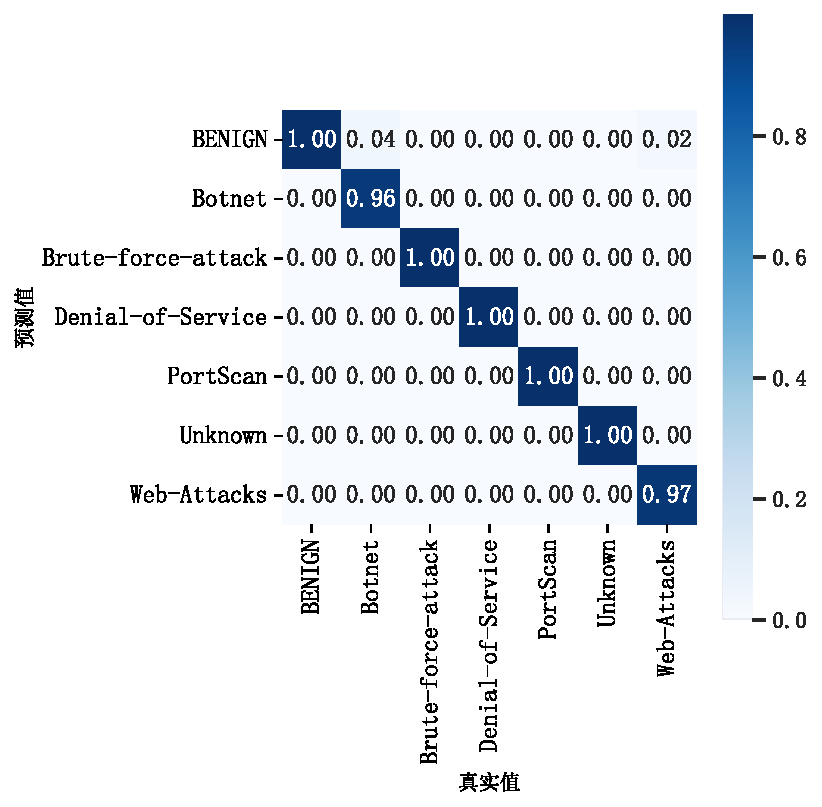
\includegraphics[width=1\linewidth]{img/exp1/4text-tr-none_confusion_matrix.pdf}
\label{fig:text-tr-none_cm}
\end{minipage}
}

\subfloat[绝对位置编码]{ % 插入第三个子图及其标题
\begin{minipage}{0.45\linewidth}
\centering
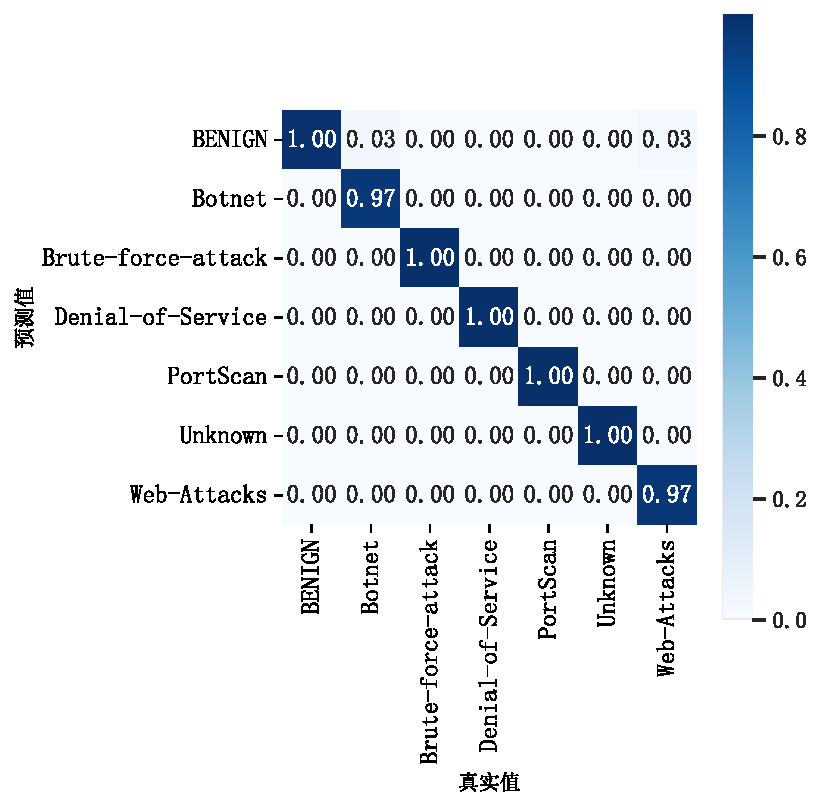
\includegraphics[width=1\linewidth]{img/exp1/5abs-tr-none_confusion_matrix.pdf}
\label{fig:abs-tr-none_cm}
\end{minipage}%
}
\subfloat[可学习位置编码]{ % 插入第四个子图及其标题
\begin{minipage}{0.45\linewidth}
\centering
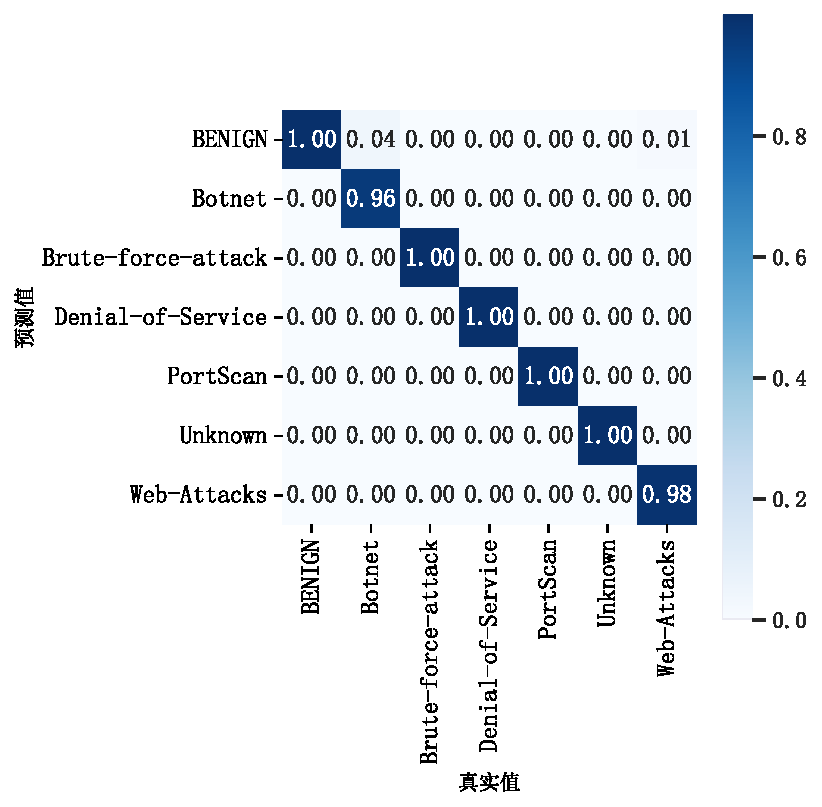
\includegraphics[width=1\linewidth]{img/exp1/6learned-tr-none_confusion_matrix.pdf}
\label{fig:learned-tr-none_cm}
\end{minipage}
}
\caption{基于不同位置编码模型的混淆矩阵} % 整个figure的标题
\label{fig:pe-tr-none_confusion_matrix}

\end{figure}

从混淆矩阵图\ref{fig:pe-tr-none_confusion_matrix}可看出分类模型对每一类样本的分类能力。这三种分类模型对于样本数量最多的4种类别(正常样本,端口扫描,拒绝服务,暴力攻击)达到了99\%以上的识别准确率。全部类别中三种模型对机器人网络流量的识别准确率均最低。

从以上的三个实验可看出,不同的位置编码对于非时序模型的影响较小,且使用文本生成的位置编码并无显著优势,反而总体准确率最低。这可能是因为生成的该编码本身性能较弱,也可能是受制于模型结构,该编码的性能并未完全展现。因此尽管本章并不对时序模型进行深入探讨,但为进一步验证不同时间编码的性能,以及为下一章内容进行预实验,会在这三种模型的基础上再加入4层Transformer进行时序建模实验。

\begin{table}[!ht]
    \centering
    \caption{增加时序Transformer后基于不同位置编码的通用编码器在CIC-IDS2017数据集上的表现}
    \begin{adjustbox}{max width=.75\textwidth}
    \begin{tabular}{lllll}
    \toprule
        编码形式 & ~ & 文本生成 & 余弦编码  &可学习  \\ \midrule
        precision & BENIGN & 0.9994  & 0.9994  & \textbf{0.9969} \\
        precision & Web-Attacks & \textbf{0.9071} & 0.6667  & 0.7000  \\
        precision & Botnet & \textbf{0.6729} & 0.4670  & 0.4904  \\
        precision & PortScan & 0.9942  & 0.9932  & \textbf{0.9947} \\
        precision & Unknown & 0.2500  & 0.1250  & \textbf{0.6205} \\
        precision & Denial-of-Service & \textbf{0.9986} & 0.9975  & 0.9982  \\
        precision & Brute-force-attack & \textbf{0.9267} & 0.7999  & 0.7758  \\
        recall & BENIGN & \textbf{0.9984} & 0.9962  & 0.9963  \\
        recall & Web-Attacks & \textbf{0.9791} & 0.9499  & 0.9652  \\
        recall & Botnet & \textbf{0.9908} & 0.9707  & 0.9835  \\
        recall & PortScan & 0.9956  & \textbf{0.9989} & 0.9968  \\
        recall & Unknown & \textbf{0.8571} & 0.7143  & 0.7143  \\
        recall & Denial-of-Service & 0.9987  & 0.9977  & \textbf{0.9994} \\
        recall & Brute-force-attack & 0.9964  & 0.9954  & \textbf{0.9968} \\
        f1 & BENIGN & \textbf{0.9989} & 0.9978  & 0.9980  \\
        f1 & Web-Attacks & \textbf{0.9417} & 0.7835  & 0.8115  \\
        f1 & Botnet & \textbf{0.8015} & 0.6306  & 0.6545  \\
        f1 & PortScan & 0.9949  & \textbf{0.9960} & 0.9957  \\
        f1 & Unknown & 0.3871  & 0.2128  & \textbf{0.6667} \\
        f1 & Denial-of-Service & 0.9987  & 0.9976  & \textbf{0.9988} \\
        f1 & Brute-force-attack & \textbf{0.9602} & 0.8870  & 0.8726  \\
        val/acc1 & all & \textbf{0.9983} & 0.9965  & 0.9968  \\
        \bottomrule
    \hline
    \end{tabular}
    \end{adjustbox}
    \label{tab:pe-tr-tr}
\end{table}

\begin{figure}[htbp] % 创建一个新的figure环境
\centering % 居中对齐所有的子图

\subfloat[文本生成位置编码]{ % 插入第二个子图及其标题
\begin{minipage}{0.5\linewidth}
\centering
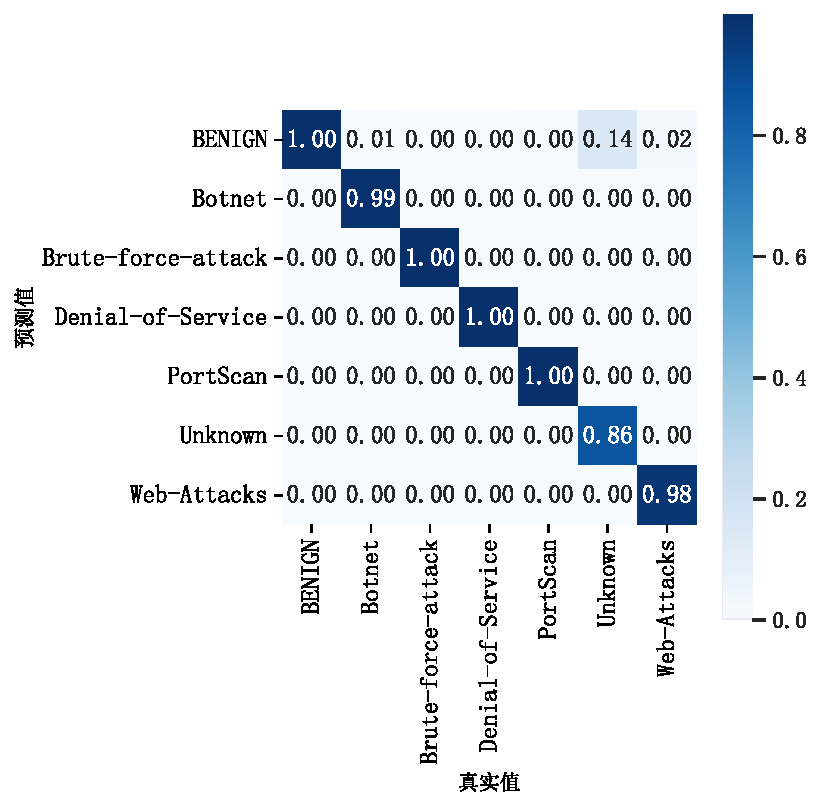
\includegraphics[width=1\linewidth]{img/exp1/1text-tr-tr_confusion_matrix.pdf}
\label{fig:1text-tr-tr_confusion_matrix}
\end{minipage}
}

\subfloat[绝对位置编码]{ % 插入第三个子图及其标题
\begin{minipage}{0.5\linewidth}
\centering
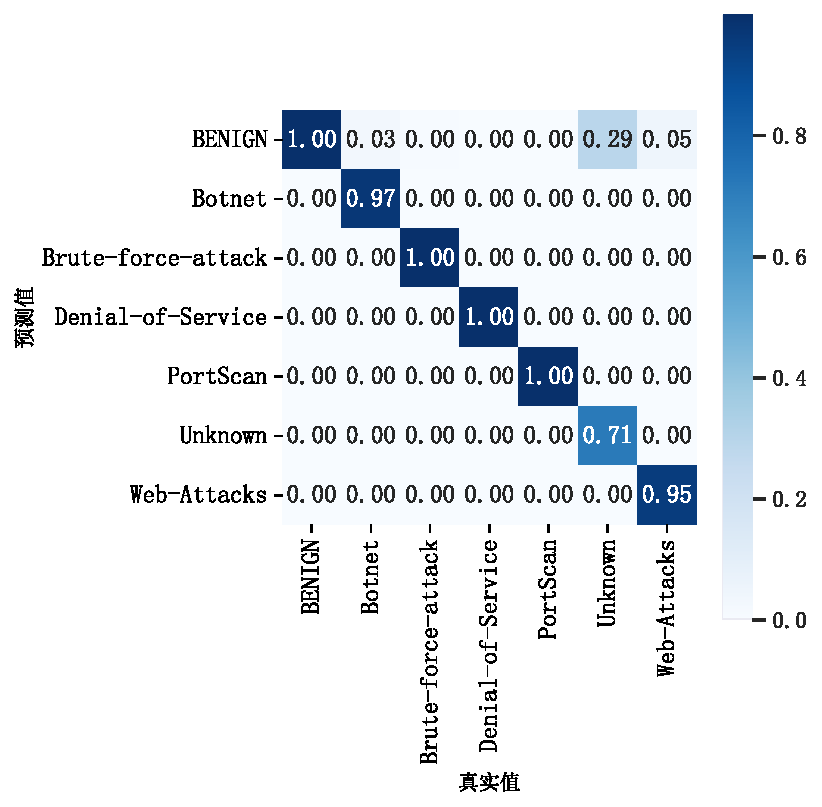
\includegraphics[width=1\linewidth]{img/exp1/2abs-tr-tr_confusion_matrix.pdf}
\label{fig:2abs-tr-tr_confusion_matrix}
\end{minipage}%
}
\subfloat[可学习位置编码]{ % 插入第四个子图及其标题
\begin{minipage}{0.5\linewidth}
\centering
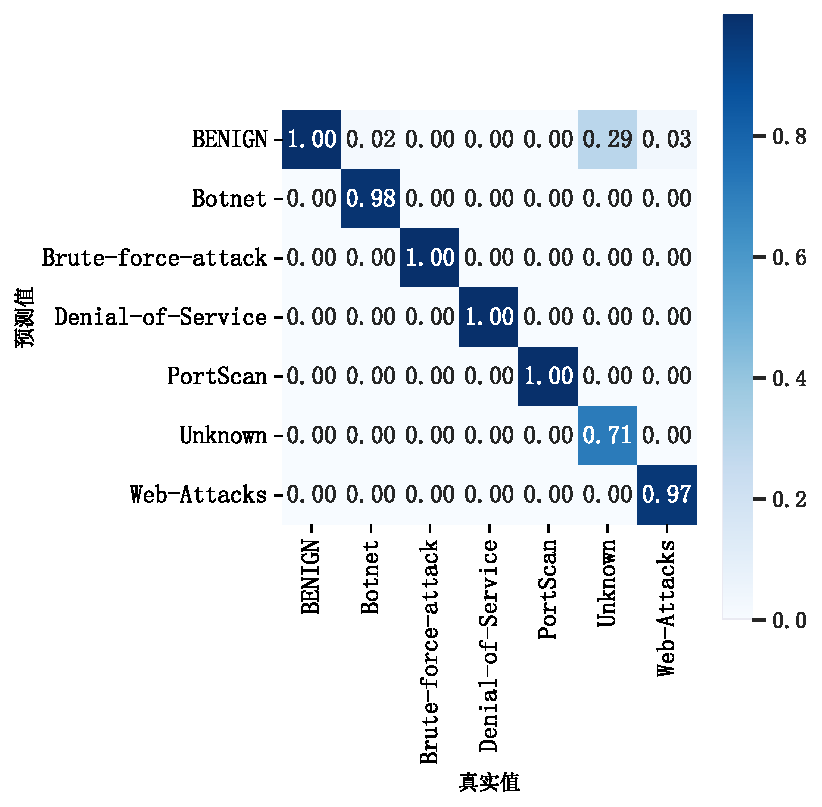
\includegraphics[width=1\linewidth]{img/exp1/3learned-tr-tr_confusion_matrix.pdf}
\label{fig:3learned-tr-tr_confusion_matrix}
\end{minipage}
}
\caption{增加时序Transformer后基于不同位置编码模型的混淆矩阵} 
\label{fig:pe-tr-tr_confusion_matrix}
\end{figure}

由表\ref{tab:pe-tr-tr}示,在通用编码器加时序模型的架构下,使用可学习位置编码以及绝对位置编码的两种模型,其识别准确率仍与原来架构相似,而使用文本生成的位置编码性能得到显著上升,综合准确率达到99.83\%。这说明使用基于文本生成的位置编码,有助于提升模型预测性能。如图\ref{fig:pe-tr-tr_confusion_matrix},从各小类的指标上分析,基于文本的位置编码在各小类别的数据表现性能上也显著优于可学习位置编码以及绝对位置编码。

\subsection{可视化分析}
位置编码为128维的向量,将不同位置的编码计算余弦相似度如图\ref{fig:pe_vis}示。从该图可看出,网络流量的第4个特征“Flow duration”与其他特征截然不同,相关度很低。位置编码沿对角线对称,相似语义的属性,其对应的位置编码也相似,如右下角,从第70个属性至最后一个属性均描述网络流量活动与空闲时间。从数据集的描述中可分析出相似的属性会被放置在相近的位置,但从该识别码可看出存在例外即数据特征的57-61维中,第59维‘Fwd Avg Bulk Rate’(前向方向的平均批量率) 与其他4个属性似乎关系较小,特别是之后的两个维度特征“后向方向的平均字节数批量率”和“后向方向的平均数据包批量率”,相差两个单词,后两维描述的方向与该特征不同,这说明网络流量具有单向性以及不对称性。

\begin{figure}[htbp]
    \centering
    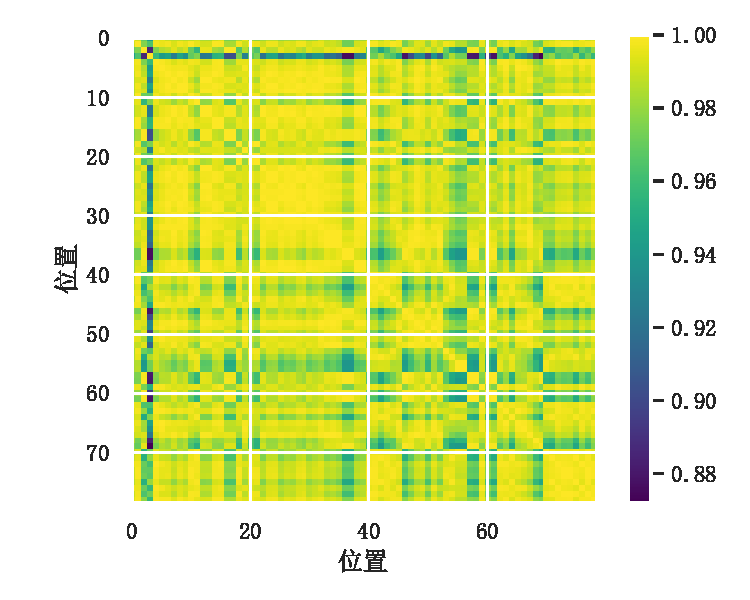
\includegraphics[width=0.75\linewidth]{img/multimodal/none-tr-tr-positional_encoding.pdf}
    \caption{位置编码可视化}
    \label{fig:pe_vis}
\end{figure}

\section{本章小结}

文章提出了一种基于多模态的入侵检测模型,该模型能有效融合网络流量属性值以及对该属性的描述信息,实现文本辅助建模。

在模型单层结构小节,重点介绍了语言辅助建模的两个关键步骤:重编码以及位置编码。前者将流量特征中的数值类型与文本类型映射为统一的128位向量,后者利用数据集中对属性的描述信息生成富含语义的位置编码,帮助模型识别每一个元素的具体含义。随后总结了语言辅助建模的整体过程,即将重编码后的结果与位置编码进行融合,从而得到输入Transformer编码器的向量。随后介绍了模型的其他组成部分,说明了各个部分的作用。

之后说明了模型的训练方法,及如何使用加权交叉熵函数实现不平衡样本的有效训练,以及如何使用AdamW 优化器进行参数更新。

最后通过实验证明了本章提出方法的有效性,最高可提升0.19\%的准确率,说明引入属性描述信息可以提高模型对网络流量建模的准确性。
\chapter{基于时序建模的入侵检测}
本章节主要介绍如何对网络流量进行时序建模以实现入侵检测。网络流量是一种时序数据,网络入侵往往包含一系列的步骤,其进行顺序存在先后关系。入侵检测是基于异常进行检测,入侵行为往往会导致网络流量特征突然发生改变,通过进行时序分析可识别这些非正常的流量模式,实现对网络入侵的高效检测。

本章将会在前一章节已提取单个网络流量特征的前提下,进一步使用时序模型进行建模。

\section{基于RNN的时序建模}
RNN是进行时序建模的经典模型,过去大部分对网络入侵进行时序建模,都使用该模型及其对应的改进形式。该模型最大特点是内部维持隐状态,而输入序列会依次输入其中,隐状态会随输入而不断变化从而保留之前输入中的有效信息。
\subsection{标准RNN介绍}
\begin{figure}[htbp]
    \centering
    \includesvg[width=.67\textwidth,keepaspectratio]{img/sequence/rnn.svg}
    \caption{RNN的神经网络结构\cite{zhang2023dive}}
    \label{fig:rnn_struct}
\end{figure}
如图\ref{fig:rnn_struct}示,最基础的循环神经网络在t时刻只有一个隐藏状态$\mathbf{H}_{t}$,该隐藏状态由上一时刻的隐藏状态$\mathbf{H}_{t-1}$与当前时刻的输入$\mathbf{X}_{t}$决定,现在每一时刻的输出只与当前时刻的隐藏态有关,具体计算过程如下:
\begin{equation}
\begin{aligned}
\mathbf{H}_{t} &= \sigma(\mathbf{W}_{\mathrm{h}} \cdot [\mathbf{H}_{t-1}, \mathbf{X}_t] + \mathbf{b}_{\mathrm{h}})\\
\mathbf{O}_{t} &= \sigma(\mathbf{W}_{\mathrm{o}}\mathbf{H}_{t} + \mathbf{b}_{\mathrm{o}})\\
\end{aligned}
\end{equation}
其中$\mathbf{W}_{hh}$ 是前一时刻隐藏状态对当前时刻隐藏状态的权重矩阵,$\mathbf{W}_{xh}$ 是当前时刻输入到当前时刻隐藏状态之间的权重矩阵,$\mathbf{b}_{h}$ 是隐藏层的偏置向量,$\sigma$ 是激活函数,循环神经网络最常用的激活函数是tanh,其特点是输出范围在-1到1,均值为0。输出范围中心化有利于下一层的输入的分布保持均衡,从而提高模型稳定性。

当神经元计算得到当前时刻隐藏状态时就可计算当前时刻的输出,因为输出只与隐藏状态有关,其中$\mathbf{W}_{ho}$ 是当前时刻隐藏状态到当前时刻输出之间的权重矩阵,$\mathbf{b}_{o}$ 是输出层的偏置向量。

在标准RNN中,信息从前一时刻传至当前时刻,需要经过矩阵变换以及激活函数激活,多次传递会造成梯度消失或梯度爆炸,因此网络难以学习长距离时序依赖关系。

\subsection{长短期记忆网络}

\begin{figure}[hbtp]
    \centering
    \includesvg[width=.67\textwidth,keepaspectratio]{img/sequence/lstm.svg}
    \caption{LSTM的神经网络结构\cite{zhang2023dive}}
    \label{fig:lstm_struct}
\end{figure}

如图\ref{fig:lstm_struct}示,LSTM针对标准RNN存在的问题,使用三个门控机制(遗忘门$\mathbf{F}_t$、输入门$\mathbf{F}_t$、输出门$\mathbf{O}_t$)控制信息流动,同时引入了长期记忆单元$\mathbf{C}$,这些门控机制决定LSTM需要记忆,需要忘记以及需要输出的信息,从而解决梯度爆炸或消失的问题,其具体计算过程如下:

\begin{enumerate}
    \item 遗忘门$\mathbf{F}_t$决定需要记忆与忘记的信息。
    \item 输入门$\mathbf{I}_t$决定当前时刻输入$X_t$中需要保留到记忆单元$\mathbf{C}$中的信息。
    \item 输出门$\mathbf{O}_t$决定当前时刻输出值。
    \item 候选记忆 $\mathbf{C}'_t$  是从短期记忆中需要被转移至长期记忆的信息。 
    \item 记忆单元$\mathbf{C}_t$由候选记忆以及上一时刻的记忆单元信息更新
    \item 隐状态$\mathbf{H}_t$,由输出门和记忆单元决定
\end{enumerate}

\begin{equation}
\begin{aligned} 
\mathbf{F}_t &= \sigma(\mathbf{W}_{\mathrm{f}} \cdot [\mathbf{H}_{t-1}, X_t] + \mathbf{b}_{\mathrm{f}})\\ 
\mathbf{I}_t &= \sigma(\mathbf{W}_{\mathrm{i}} \cdot [\mathbf{H}_{t-1}, X_t] + \mathbf{b}_{\mathrm{i}})\\ 
\mathbf{O}_t &= \sigma(\mathbf{W}_{\mathrm{o}} \cdot [\mathbf{H}_{t-1}, X_t] + \mathbf{b}_{\mathrm{o}})\\ 
\mathbf{C}'_t &= \tanh(\mathbf{W}_C \cdot [\mathbf{H}_{t-1}, X_t] + \mathbf{b}_C)\\ 
\mathbf{C}_t &= \mathbf{F}_t \ast \mathbf{C}_{t-1} + \mathbf{I}_t \ast \mathbf{C}'_t\\ 
\mathbf{H}_t &= \mathbf{O}_t \ast \tanh(\mathbf{C}_t)\\ 
\end{aligned}
\end{equation}

其中,$\sigma$为sigmoid函数,将门控的输出值的大小控制在0和1之间,$\ast$表示Hadamard积,即元素对元素的乘积;$W$和$b$分别代表映射矩阵和对应的偏置向量,下标$f$、$i$、$C$和$o$分别表示遗忘门、输入门、候选长期记忆和输出门。

LSTM通过门控机制一定程度上解决了长序列中的梯度爆炸与消失问题,但其结构过于复杂,每个神经元内的计算步骤多,消耗计算资源大。

\subsection{基于门控神经元的循环神经网络}
\begin{figure}[htbp]
    \centering
    \includesvg[width=.67\textwidth,keepaspectratio]{img/sequence/gru.svg}
    \caption{GRU的神经网络结构\cite{zhang2023dive}}
    \label{fig:gru_struct}
\end{figure}

如图\ref{fig:gru_struct}示,GRU对LSTM进行一定程度的简化,在避免梯度异常的同时降低了模型的计算量。其使用两个门控机制(重置门$\mathbf{R}_t$、更新门$\mathbf{Z}_t$)进行信息选择,主要更新过程如下:
\begin{enumerate}
    \item 更新门$\mathbf{Z}_t$控制状态更新时前一时刻隐状态$\mathbf{H}_{t-1}$中信息的保留。
    \item 重置门$\mathbf{R}_t$决定计算候选隐藏状态$\tilde{\mathbf{H}}_t$ 时对前一时刻隐藏状态$\mathbf{H}_{t-1}$的参考程度。
    \item 候选隐藏状态$\tilde{\mathbf{H}}_t$ 由前一时刻隐藏状态$\mathbf{H}_{t-1}$和当前时刻输入$\mathbf{X}_t$决定。
    \item 最终隐藏状态$\mathbf{H}_t$由前一时刻隐藏状态$\mathbf{H}_{t-1}$以及当前时刻候选隐藏状态$\tilde{\mathbf{H}}_t$ 决定。
\end{enumerate}

\begin{equation}
    \begin{aligned}
        \mathbf{Z}_t &= \sigma(\mathbf{W}_{\mathrm{z}} \cdot [\mathbf{H}_{t-1}, \mathbf{X}_t] + \mathbf{b}_{\mathrm{z}})\\
        \mathbf{R}_t &= \sigma(\mathbf{W}_r \cdot [\mathbf{H}_{t-1}, \mathbf{X}_t] + \mathbf{b}_{\mathrm{r}})\\
        \tilde{\mathbf{H}}_t &= \tanh(\mathbf{W}_{\mathrm{h}} \cdot [\mathbf{R}_t \ast \mathbf{H}_{t-1}, \mathbf{X}_t] + \mathbf{b}_{\mathrm{h}})\\
        \mathbf{H}_t &= \mathbf{Z}_t \ast \mathbf{H}_{t-1} + (1 - \mathbf{Z}_t) \ast \tilde{\mathbf{H}}_t
    \end{aligned}   
\end{equation}

其中,$\sigma$与LSTM中的门控机制激活函数相同为sigmoid;$W$和$b$分别表示投影矩阵和对应的偏置向量,下标$z$、$r$和$h$分别代表更新门、重置门和候选隐藏状态。

GRU简化了LSTM的门控机制,减少了模型的参数量与计算量,虽然其长序列建模能力弱于LSTM,但在计算资源有限的情况下可作为其近似替代。

\section{基于Transformer的时序建模}
Transformer架构已在上一章节进行详细介绍。该架构有很多特点,上一章节主要利用其可伸缩性以及灵活性实现多模态建模,且多模态模型在获得数据各属性文本描述的情况下,可兼容任何格式数据集。

本章将继续利用该架构进行时序建模。相比上一节介绍的基于RNN及改进形式的时序建模,基于Transformer的时序建模在网络入侵领域检测领域更合适,特别是针对一些时间跨度较大的网络攻击方式。在KDDCUP-99数据集中的Slowloris就是一种经典的低速攻击,通过缓慢发送HTTP请求,实现占有服务器资源的目的。较新的勒索软件攻击,也是一种需要进行长距离建模的网络入侵,它包含多个步骤,从开始渗透到最终完成对文件的加密并发送密钥,会间隔较长时间。

\section{基于时序建模的入侵检测模型}
在上一章提出了一种基于文本辅助的分类模型,模型包括编码与分类两部分,文章将会继续使用其中编码部分$F_{encoder}$,编码器将任意格式的网络流量特征映射为128维的向量。另一方面为方便模型分析与对比,本章将会使用线性编码器,该编码器实际为投影矩阵$Porj_{encoder}$,可将流量特征线性映射至128维。

在处理网络数据包时需考虑每个数据包本身的上下文无关特征,以及其在时间序列中的上下文信息,本节采用两阶段的处理流程。第一步,通过一定的特征提取方法(非线性编码或线性编码)获得每个数据包的上下文无关特征$\mathbf{z}_{\mathrm{cls}}$,该特征为一定长向量。第二步,为了捕捉时间序列中的上下文关联性,分别使用基于RNN或使用Transformer的时序的模型进行上下文建模。

基于Transformer的时序建模过程如算法\ref{alg:transformer_serial}示。

\begin{algorithm}[htb]
\caption{四层Transformer时序建模算法}
\begin{algorithmic}
\REQUIRE 定长序列 $S$,其中 $S$ 是一个 $N \times 128$ 的矩阵,$N$ 表示序列长度
\ENSURE 等长序列 $S'$,输出序列也是一个 $N \times 128$ 的矩阵

\STATE 分割 $S$ 为若干个长度为 $L$ 的序列片段 $\{S_1, S_2, \ldots, S_k\}$
\STATE 对每个序列片段 $S_i$,引入可学习的令牌 $\mathbf{T} = \{\mathbf{t}_1, \mathbf{t}_2, \ldots, \mathbf{t}_m\}$
\STATE 初始化四层Transformer模型 $Trans_1, Trans_2, Trans_3, Trans_4$
\FOR{$i = 1$ 到 $4$}
    \IF{$i == 1$}
        \STATE $input \gets [\mathbf{T}; S_i]$  \COMMENT{第一层的输入包括令牌和序列片段}
    \ELSE
        \STATE $input \gets output$  \COMMENT{后续层的输入为前一层的输出}
    \ENDIF
    \STATE $output \gets Trans_i(input)$ \COMMENT{使用Transformer层处理输入}
    \IF{$i == 4$}
        \STATE 移除输入中的可学习令牌 $\mathbf{T}$,保留序列信息得到 $S'$
    \ENDIF
\ENDFOR
\RETURN $S'$
\end{algorithmic}
\label{alg:transformer_serial}
\end{algorithm}

本章同样使用四层Transformer对数据流量进行时序建模。与RNN不同Transformer的注意力机制中计算复杂度与序列的长度呈平方关系而不是线性关系,因此在算法的第1步会将网络流量切为长度相同的短片段,若数据预处理中已对数据进行分割,则此步不必进行。对于分割后的子序列,算法会在序列头部加入特殊向量,该向量用于表示整个序列的上下文信息。

在算法的执行过程中,Transformer的每一层输入都会作为下一层的输出,以此实现模型对流量特征的提取。在最后一层算法会移除之前加入的头部特殊向量,得到与源序列等长部分并输出。



\begin{enumerate}
\item 时间序列分段
   
   对于一个时间序列数据,例如由网络数据包组成的序列,首先将其划分为长度相同的子序列,这些子序列不应该有重叠。设定一个序列片段的长度为 $L$(也就是窗口大小),则原时间序列可以被分为若干个长度为 $L$ 的序列片段:

   \begin{equation}
          \mathbf{S}_i = \{\mathbf{z}_{\mathrm{cls}}^{(i*L)}, \mathbf{z}_{\mathrm{cls}}^{(i*L+1)}, \ldots, \mathbf{z}_{\mathrm{cls}}^{(i*L+L-1)}\}
   \end{equation}

   其中,$\mathbf{S}_i$ 表示第 $i$ 个序列片段,$\mathbf{z}_{\mathrm{cls}}^{(j)}$ 表示第 $j$ 个数据包的上下文无关特征。

\item 引入可学习的令牌

   在输入Transformer模型之前,引入一系列可学习的令牌,可以捕获和存储全局信息。设定这些可学习的令牌集合为 $\mathbf{T} = \{\mathbf{t}_1, \mathbf{t}_2, \ldots, \mathbf{t}_m\}$,其中 $m$ 是可学习令牌的数量。这些令牌被初始化,并在训练过程中与其他参数一起更新。

\item Transformer模型

   使用一个4层的Transformer结构来处理上述拼接后的序列数据。Transformer的输入是编码器头生成的特征向量序列加上可学习的令牌。设Transformer的输出为 $\mathbf{O}$:

   \begin{equation}
   \mathbf{O} = {\mathrm{Transformer}}([\mathbf{T}; \mathbf{S}_i])
   \end{equation}

   其中,$[\mathbf{T}; \mathbf{S}_i]$ 表示令牌和序列片段的拼接。

\item 移除令牌

   在Transformer模型处理完毕后,移除步骤2中添加的可学习令牌,只保留与原始数据包对应的输出部分。这样得到的输出序列 $\mathbf{O'}$ 只包含了来自原始序列片段的信息:

   \begin{equation}
   \mathbf{O'} = \mathbf{O} \setminus \mathbf{T}
   \end{equation}
\end{enumerate}

通过以上两种时序模型可在保留数据包的独立特征的同时,学习到序列中的上下文关联。因而模型在对数据包进行分析时可通过上下文信息进行更准确的判断。

\section{实验结果}
本章是在上一章的基础上进行时序建模探索,前一章节的预实验已证明使用时序模型可提高模型的拟合能力。本小节将会对基于时序建模的模型性能进行进一步实验分析。第一步对最简单的时序模型即使用线性编码器的不同时序模型进行研究,实验平台和实验参数与上一章保持一致,只有模型不同。本小节所用线性编码器即为投影矩阵。实验结果如表\ref{tab:none-seq}示。
\begin{table}[!ht]
    \centering
    \caption{基于线性编码器的时序模型CIC-IDS2017数据集上的表现}
    \begin{adjustbox}{max width=.75\textwidth}
    \begin{tabular}{llllll}
    \toprule
        衡量指标 & 实验编号 & exp1(a) & exp2(b)  & exp3(c) & exp4(d)\\ \midrule
        时序建模方式 & ~ & RNN & LSTM & GRU  & Transformer  \\ 
        recall & BENIGN & \textbf{1} & \textbf{1} & \textbf{1} & 0.9907 \\
        recall & Web-Attacks & 0 & 0 & 0 & \textbf{0.9345} \\
        recall & Botnet & 0 & 0 & 0 & \textbf{0.8388} \\
        recall & PortScan & 0 & 0 & 0 & \textbf{0.9971} \\
        recall & Unknown & 0 & 0 & 0 & \textbf{0.8571} \\
        recall & Denial-of-Service & 0 & 0 & 0 & \textbf{0.9949} \\
        recall & Brute-force-attack & 0 & 0 & 0 & \textbf{0.9537} \\
        acc & all & 0.8037 & 0.8037 & 0.8038 & \textbf{0.9913} \\

    \bottomrule
    \end{tabular}
    \end{adjustbox}
    \label{tab:none-seq}
\end{table}

分析可得,基于RNN的时序模型均发生过拟合,除正常类别外所有其他类别召回率均为0,仅输出样本个数最多的类别即正常类别。基于Transformer架构的时序模型则正常输出,对正常样本的识别能力弱于对拒绝服务、端口扫描等样本数较多的恶意类别。

以上的实验结果说明,仅使用时序模型进行建模,并不能充分提取网络特征,因此需要将时序模型与上一章提出的通用编码器相结合,组合后的实验结果如表\ref{tab:tr-seq}示。

\begin{table}[!ht]
    \centering
    \caption{基于通用编码器的时序模型在CIC-IDS2017数据集上的表现}
    \begin{adjustbox}{max width=.75\textwidth}
    \begin{tabular}{llllll}
    \toprule
        衡量指标 & 实验编号 & exp1(a) & exp2(b)  & exp3(c) & exp4(d)\\ \midrule
        时序建模方式 & ~ & GRU & LSTM & RNN  & Transformer  \\ 
        precision & BENIGN & 0.9995  & 0.9992  & 0.9993  & \textbf{0.9996} \\
        precision & Web-Attacks & 0.7417  & 0.5573  & 0.7006  & \textbf{0.9130} \\
        precision & Botnet & 0.4693  & 0.3876  & 0.2663  & \textbf{0.6538} \\
        precision & PortScan & \textbf{0.9942}  & 0.9895  & 0.9901  & 0.9924 \\
        precision & Unknown & 0.0284  & 0.0045  & 0.0211  & \textbf{0.3158} \\
        precision & Denial-of-Service & 0.9955  & 0.9887  & 0.9931  & \textbf{0.9985} \\
        precision & Brute-force-attack & 0.8825  & 0.7444  & 0.8167  & \textbf{0.9317} \\
        recall & BENIGN & 0.9967  & 0.9931  & 0.9939  & \textbf{0.9983} \\
        recall & Web-Attacks & 0.9680  & 0.9485  & 0.9582  & \textbf{0.9791} \\
        recall & Botnet & 0.9670  & 0.9414  & 0.9597  & \textbf{0.9890} \\
        recall & PortScan & \textbf{0.9987}  & 0.9978  & 0.9979  & 0.9984 \\
        recall & Unknown & 0.5714  & 0.1429  & \textbf{0.8571}  & \textbf{0.8571} \\
        recall & Denial-of-Service & 0.9976  & 0.9964  & 0.9969  & \textbf{0.9987} \\
        recall & Brute-force-attack & 0.9951  & 0.9944  & 0.9893  & \textbf{0.9966} \\
        f1 & BENIGN & 0.9981  & 0.9961  & 0.9966  & \textbf{0.9989} \\
        f1 & Web-Attacks & 0.8399  & 0.7021  & 0.8094  & \textbf{0.9449} \\
        f1 & Botnet & 0.6320  & 0.5491  & 0.4169  & \textbf{0.7872} \\
        f1 & PortScan & \textbf{0.9964}  & 0.9936  & 0.9940  & 0.9954 \\
        f1 & Unknown & 0.0541  & 0.0088  & 0.0412  & \textbf{0.4615} \\
        f1 & Denial-of-Service & 0.9965  & 0.9926  & 0.9950  & \textbf{0.9986} \\
        f1 & Brute-force-attack & 0.9354  & 0.8514  & 0.8948  & \textbf{0.9631} \\
        acc & all & 0.9969  & 0.9937  & 0.9945  & \textbf{0.9983} \\
    \bottomrule
    \end{tabular}
    \end{adjustbox}
    \label{tab:tr-seq}
\end{table}

将表\ref{tab:tr-seq}与表\ref{tab:none-seq}对比可知,引入通用编码器,避免了模型过拟合。其中三种基于RNN都是时序网络架构均能实现正常输出。其中基于Transformer架构的时序模型分类准确度最高为99.83\%,效果最差的是LSTM
,仅为99.37\%。基于Transformer架构的时序模型在几乎全部类别的分类结果上均优于其他模型,除了端口扫描。所有基于RNN的网络结构中,效果最好的是基于GRU的网络,在端口扫描上的三项指标均优于Transformer架构。

如图\ref{fig:tr-serial_confusion_matrix}示,基于Transformer的时序建模与基于RNN的时序建模在识别小样本类别上有比较高的准确率。基于LSTM的时序模型对小样本类别,识别能力最差,仅能识别约14\%的样本。

\begin{figure}[htbp] % 创建一个新的figure环境
\centering % 居中对齐所有的子图

\subfloat[基于RNN的时序模型]{ % 插入第二个子图及其标题
\begin{minipage}{0.435\linewidth}
\centering
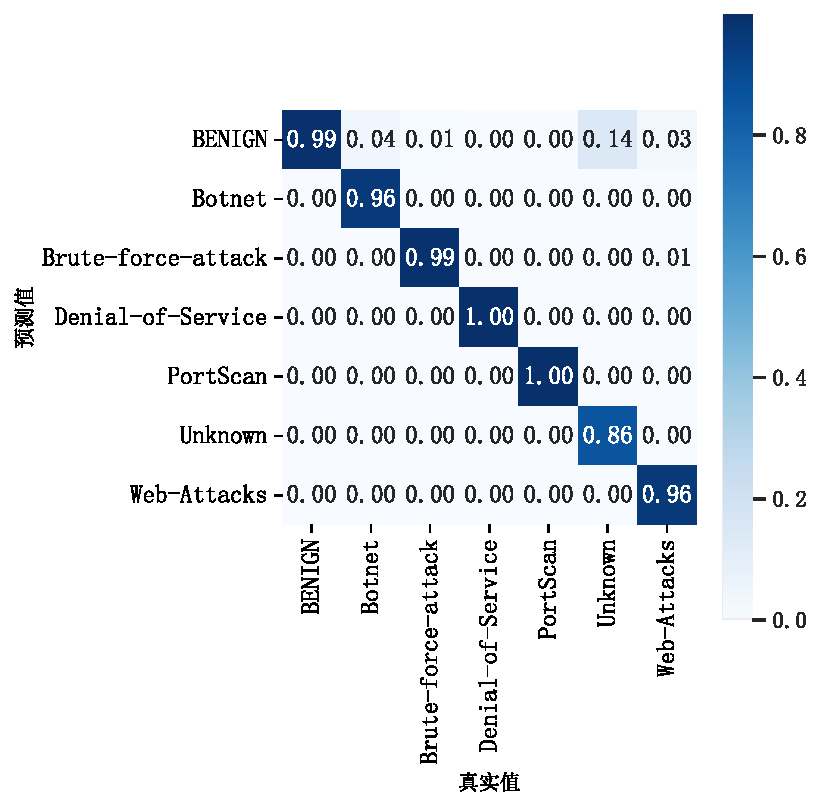
\includegraphics[width=1\linewidth]{img/exp2/3tr-rnn_confusion_matrix.pdf}
\label{fig:3tr-rnn_confusion_matrix}
\end{minipage}
}
\subfloat[基于LSTM的时序模型]{ % 插入第三个子图及其标题
\begin{minipage}{0.435\linewidth}
\centering
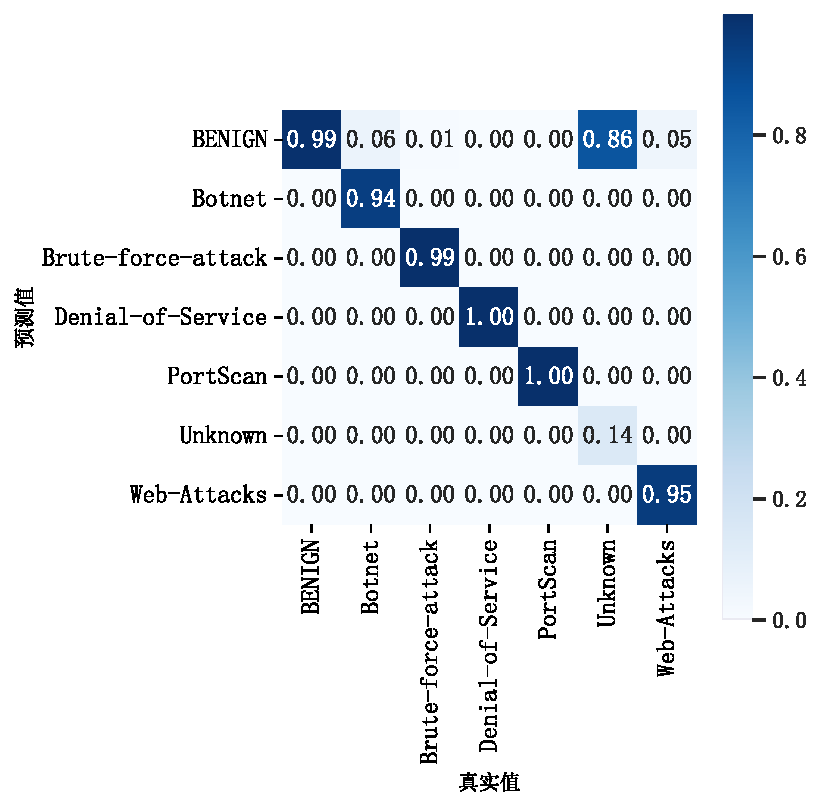
\includegraphics[width=1\linewidth]{img/exp2/5tr-lstm_confusion_matrix.pdf}
\label{fig:5tr-lstm_confusion_matrix}
\end{minipage}%
}

\subfloat[基于GRU的时序模型]{ % 插入第四个子图及其标题
\begin{minipage}{0.435\linewidth}
\centering
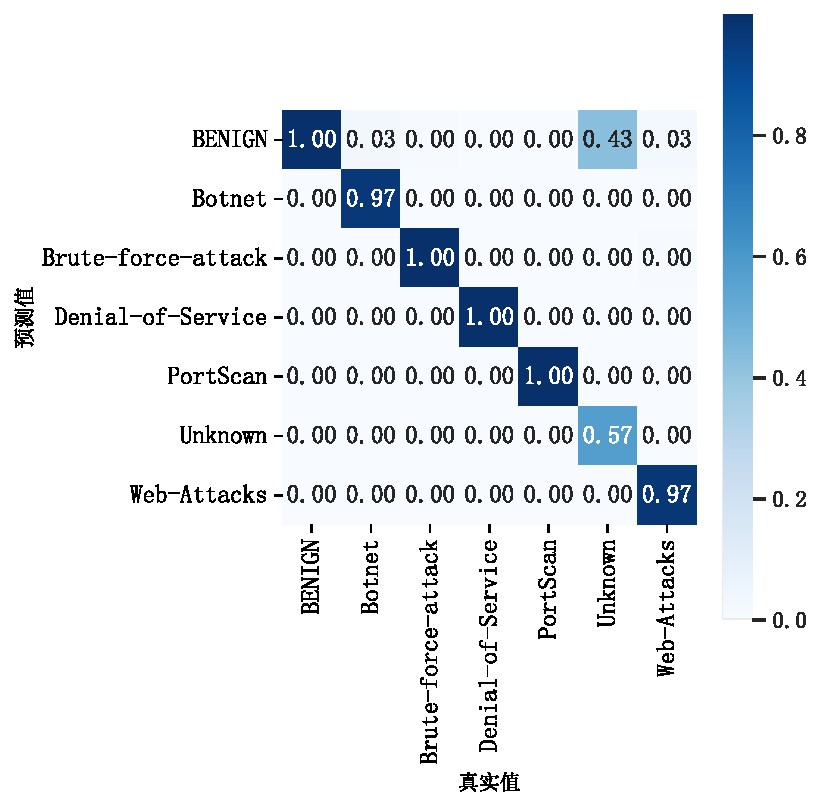
\includegraphics[width=1\linewidth]{img/exp2/7tr-gru_confusion_matrix.pdf}
\label{fig:7tr-gru_confusion_matrix}
\end{minipage}
}
\subfloat[基于Traansformer的时序模型]{ % 插入第四个子图及其标题
\begin{minipage}{0.435\linewidth}
\centering
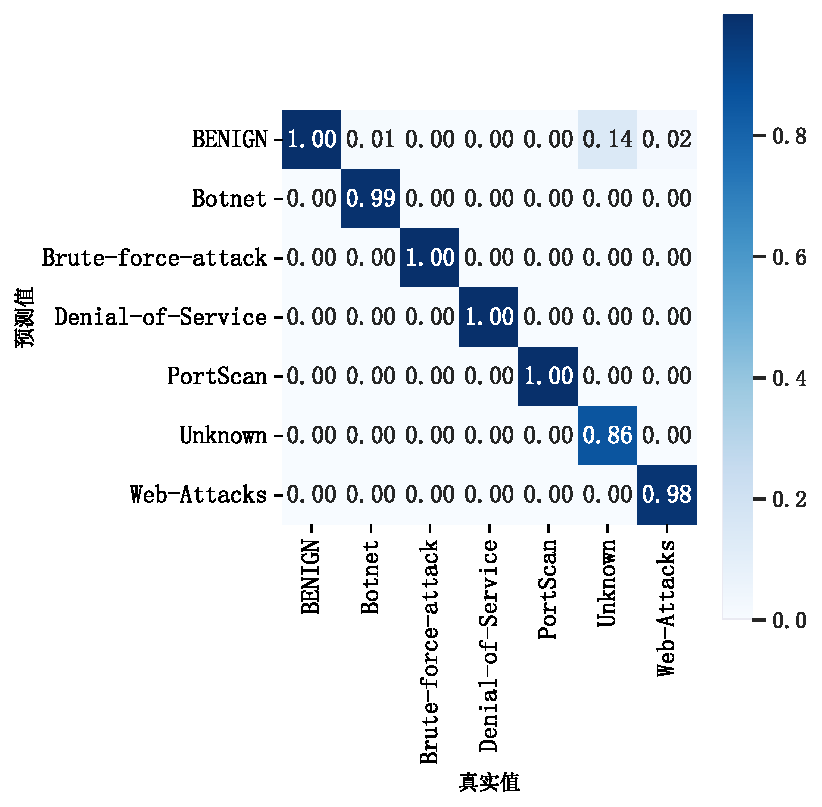
\includegraphics[width=1\linewidth]{img/exp2/1tr-tr_confusion_matrix.pdf}
\label{fig:1tr-tr_confusion_matrix}
\end{minipage}
}
\caption{使用通用编码器编码的不同时序模型混淆矩阵} % 整个figure的标题
\label{fig:tr-serial_confusion_matrix}
\end{figure}

LSTM有更复杂的门控结构,大部分任务上其性能要比GRU好。在网络入侵检测任务上性能差可能是在极度不均衡数据集上训练模型时,很难将LSTM调整到最适合的参数,而结构较为简单的GRU调节起来也较LSTM容易,可更快达到最优状态。标准RNN因其原本的特性难以对长序列建模而性能弱于GRU。

Transformer中的注意力机制在帮助模型实现长距建模的同时也提供了一种良好的可视化手段。在注意力机制中,每个头都有独立的注意力矩阵,为方便可视化,本小节仅取所有头的均值作为平均注意力值,该值反映了同一序列中两个位置的相关程度。如图\ref{fig:serial_att}示较浅层的注意力分数往往表现为平均,而最后一层的注意力分数最亮与最暗的值较多。这说明通过注意力机制模型,原有的预测被不断纠正,并最终接近实际标签。

\begin{figure}[htbp] % 创建一个新的figure环境
\centering % 居中对齐所有的子图

\subfloat[第1层注意力矩阵]{ % 插入第二个子图及其标题
\begin{minipage}{0.5\linewidth}
\centering
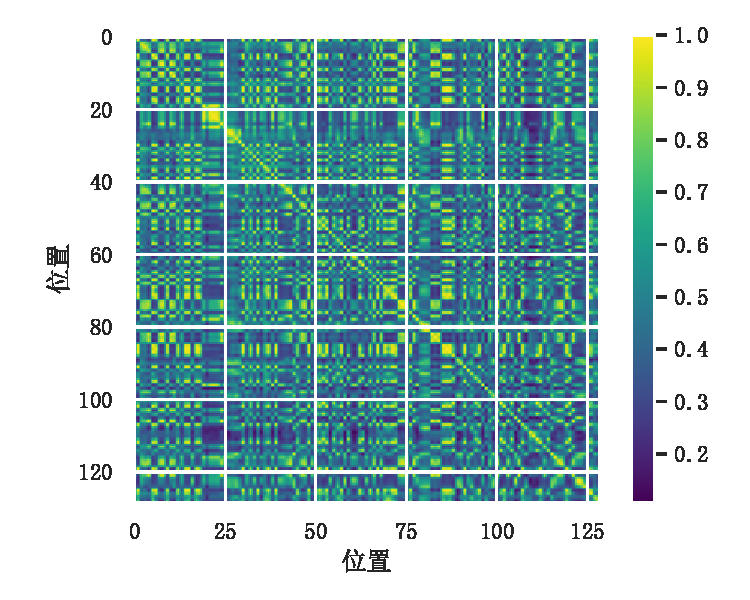
\includegraphics[width=1\linewidth]{img/sequence/att0.pdf}
\label{fig:serial_att_1}
\end{minipage}
}
\subfloat[第4层注意力矩阵]{ % 插入第三个子图及其标题
\begin{minipage}{0.5\linewidth}
\centering
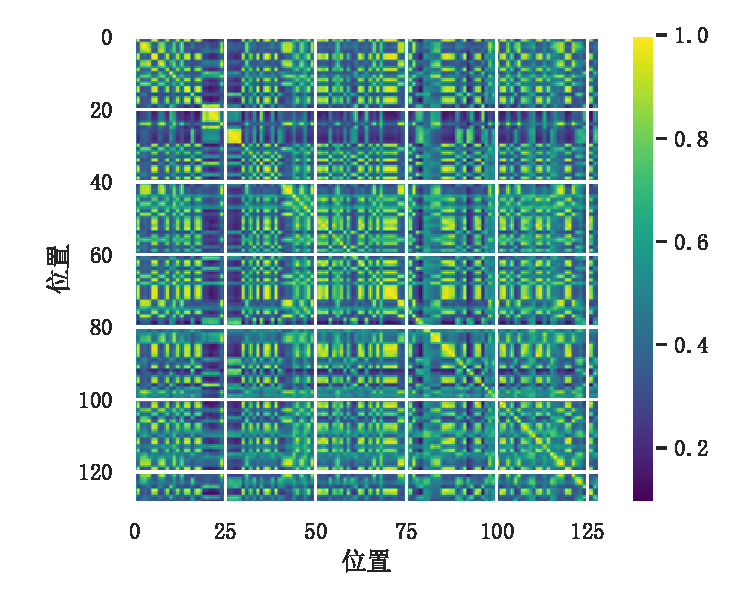
\includegraphics[width=1\linewidth]{img/sequence/att3.pdf}
\label{fig:serial_att_4}
\end{minipage}%
}

\caption{基于Transformer的时序模型注意力可视化} % 整个figure的标题
\label{fig:serial_att}
\end{figure}

实验证明对网络流量使用上一章提出的语言辅助编码器进行统一编码后,再使用时序模型进行时序建模,可得到更高的准确率。具体建模过程如图\ref{fig:overview}示。
\begin{figure}[htb]
    \centering
    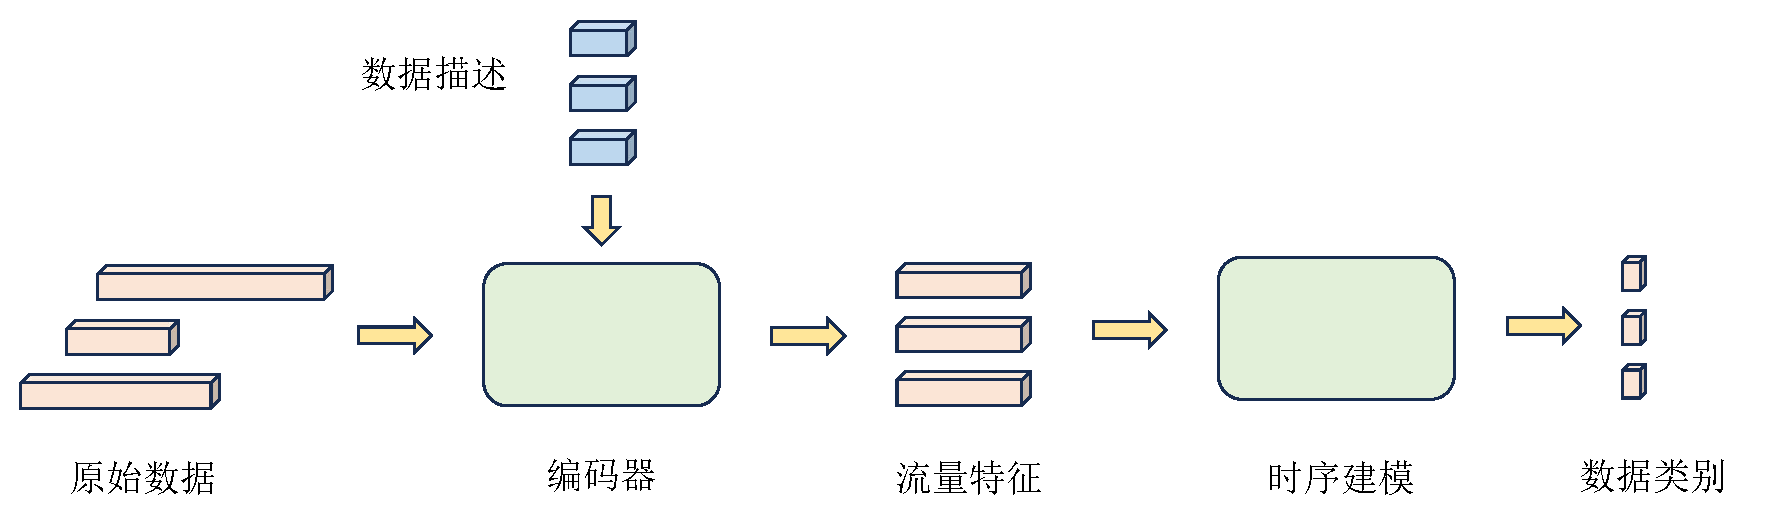
\includegraphics[width=\textwidth,height=\textheight,keepaspectratio]{img/overview.pdf}
    \caption{基于语言辅助编码器的时序模型}
    \label{fig:overview}
\end{figure}
网络由两部分组成,在第1步对不同类型的数据,结合数据本身的特征和对特征的文字描述,使用编码器形成对这些数据的编码即流量特征。第二步是结合数据的上下文特征进行时序建模,并根据建模结果得到这些数据对应的类别。

与近期方法比较如表\ref{tab:trm_cic2017_compare}示,本章提出的方法在CIC-IDS2017数据集上具有一定的先进性。

\begin{table}[htb]
    \centering
    \caption{CIC-IDS2017数据集上与其他方法对比}
    \begin{tabular}{lll}
    \toprule
        模型 & 分类数 & 准确率 \\ \midrule
        本章提出的方法 & 7 & 99.83\% \\ 
        LUCID\cite{10.1109/TNSM.2020.2971776}& 2 & 99.66\% \\ 
        CNN+LSTM\cite{10.1109/CCWC.2019.8666588}& 2 & 98.44\% \\
        MECNN\cite{10.1016/j.knosys.2022.108505}& 7& 99.73\%\\ 
        \bottomrule
    \end{tabular}
    \label{tab:trm_cic2017_compare}
\end{table}

\section{本章小结}
本章对基于时序建模的入侵检测模型进行研究,并对不同结构的时序模型进行实验,分析其在 CIC-IDS2017数据集上的性能与效果。

在本章节的开始对经典RNN及其改进形式进行了介绍,随后提出了基于Transformer的时序检测模型。通过三种RNN与Transformer进行对比发现,基于Transformer入侵检测模型在CIC-IDS2017这种数据分布极不均衡的数据集上具有较好的拟合能力。其他三种RNN出现了过拟合现象,对于全部样本仅输出数量最多的类别即正常类别,而基于Transformer性能表现弱于上一章节提出的针对单个流量的多模态入侵检测。

以上4种模型加入前一章提出的多模态入侵检测编码器后,三种RNN过拟合现象得到明显改善,可对各种类别的样本进行正确分类。而使用Transformer的模型实现了更高的准确率(提升了0.7\%)。之后通过可视化分析,对该模型中注意力机制上的时序原理进行分析,证实了在流量分类中的作用。本章节提出并验证了一个有效的网络入侵检测模型。

\chapter{基于迁移学习的入侵检测}
之前的章节都是在已有的数据集上进行实验,所得的基于Transformer的模型已经实现了对网络威胁的准确发现。
然而实际的网络环境与训练所使用的开源数据集有所不同,此差异会导致模型识别准确率下降;另一方面随着网络技术的发展,新的攻击方式会不断出现,这对于二分类模型会降低其准确率,而对于多分类模型,可能会导致其完全失效。此外,实际部署情况下,出于对成本的考虑,在目标网络数据集上只能获得较少已标注数据。

迁移学习可充分利用模型从已有数据集中学到的知识,从而调整模型,使模型适应目标网络环境,以低的计算成本,低的数据标注需求达到较高的准确率。

本章节将以CIC-IDS2017为源数据集,KDDCUP-99数据集为目标数据集进行迁移学习,这两个数据集的格式不同,数据集中存在的攻击类别也不同。目的是以尽可能少的目标数据集数据量实现尽可能高的识别准确率。

\section{基于模型微调的迁移学习}
\begin{figure}
    \centering
    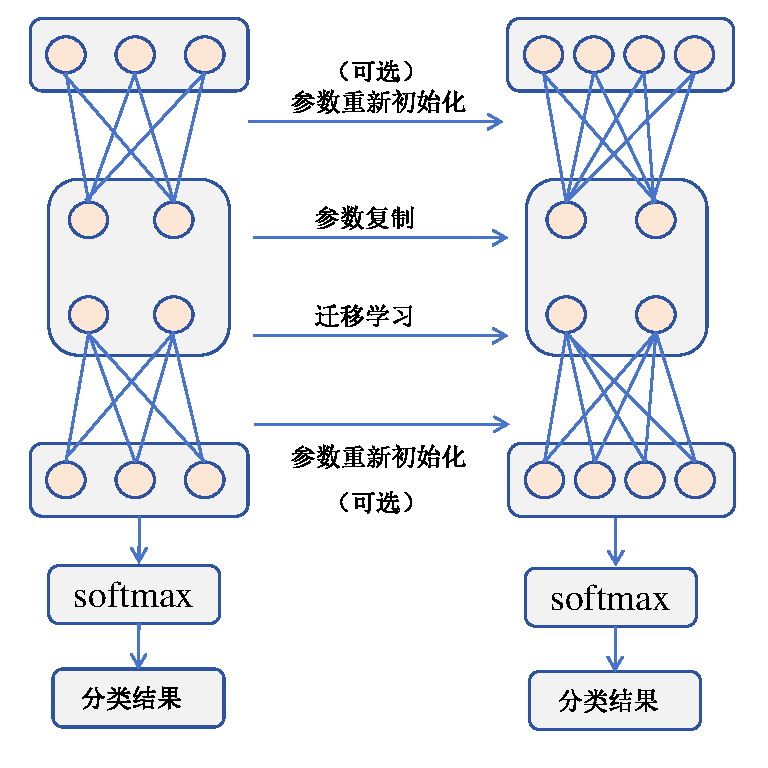
\includegraphics[height=.25\textheight,keepaspectratio]{img/transfer/model_transfer.pdf}
    \caption{模型迁移学习方法}
    \label{fig:model_transfer}
\end{figure}
基于模型微调的迁移学习方法如图\ref{fig:model_transfer}示。当原数据及格式与目标数据集不相同时,需要对模型的结构进行调整。

若输入维度不匹配,通常情况会调整神经网络的第1层,这主要是因为神经网络中靠近输入层的权重往往与数据集中低层次信息有关,当数据集发生变化及低层次语义信息会显著发生变化,原数据集中的权重将不再适用。如果在多分类任务中输出维度不匹配,则会调整神经网络的最后一层,这主要是因为最后一层的输出直接关联具体任务,其维度即为输出的类别数。

本节使用的模型沿用上一章节使用线性编码的模型,当输入的维度发生变化时会丢弃原有的投影矩阵,然后使用新的特征矩阵,实现维度匹配;执行多分类任务时,若样本类别不同则丢弃最后一层全连接层,然后将其进行随机初始化。
\section{基于模型微调的迁移学习}
\begin{figure}
    \centering
    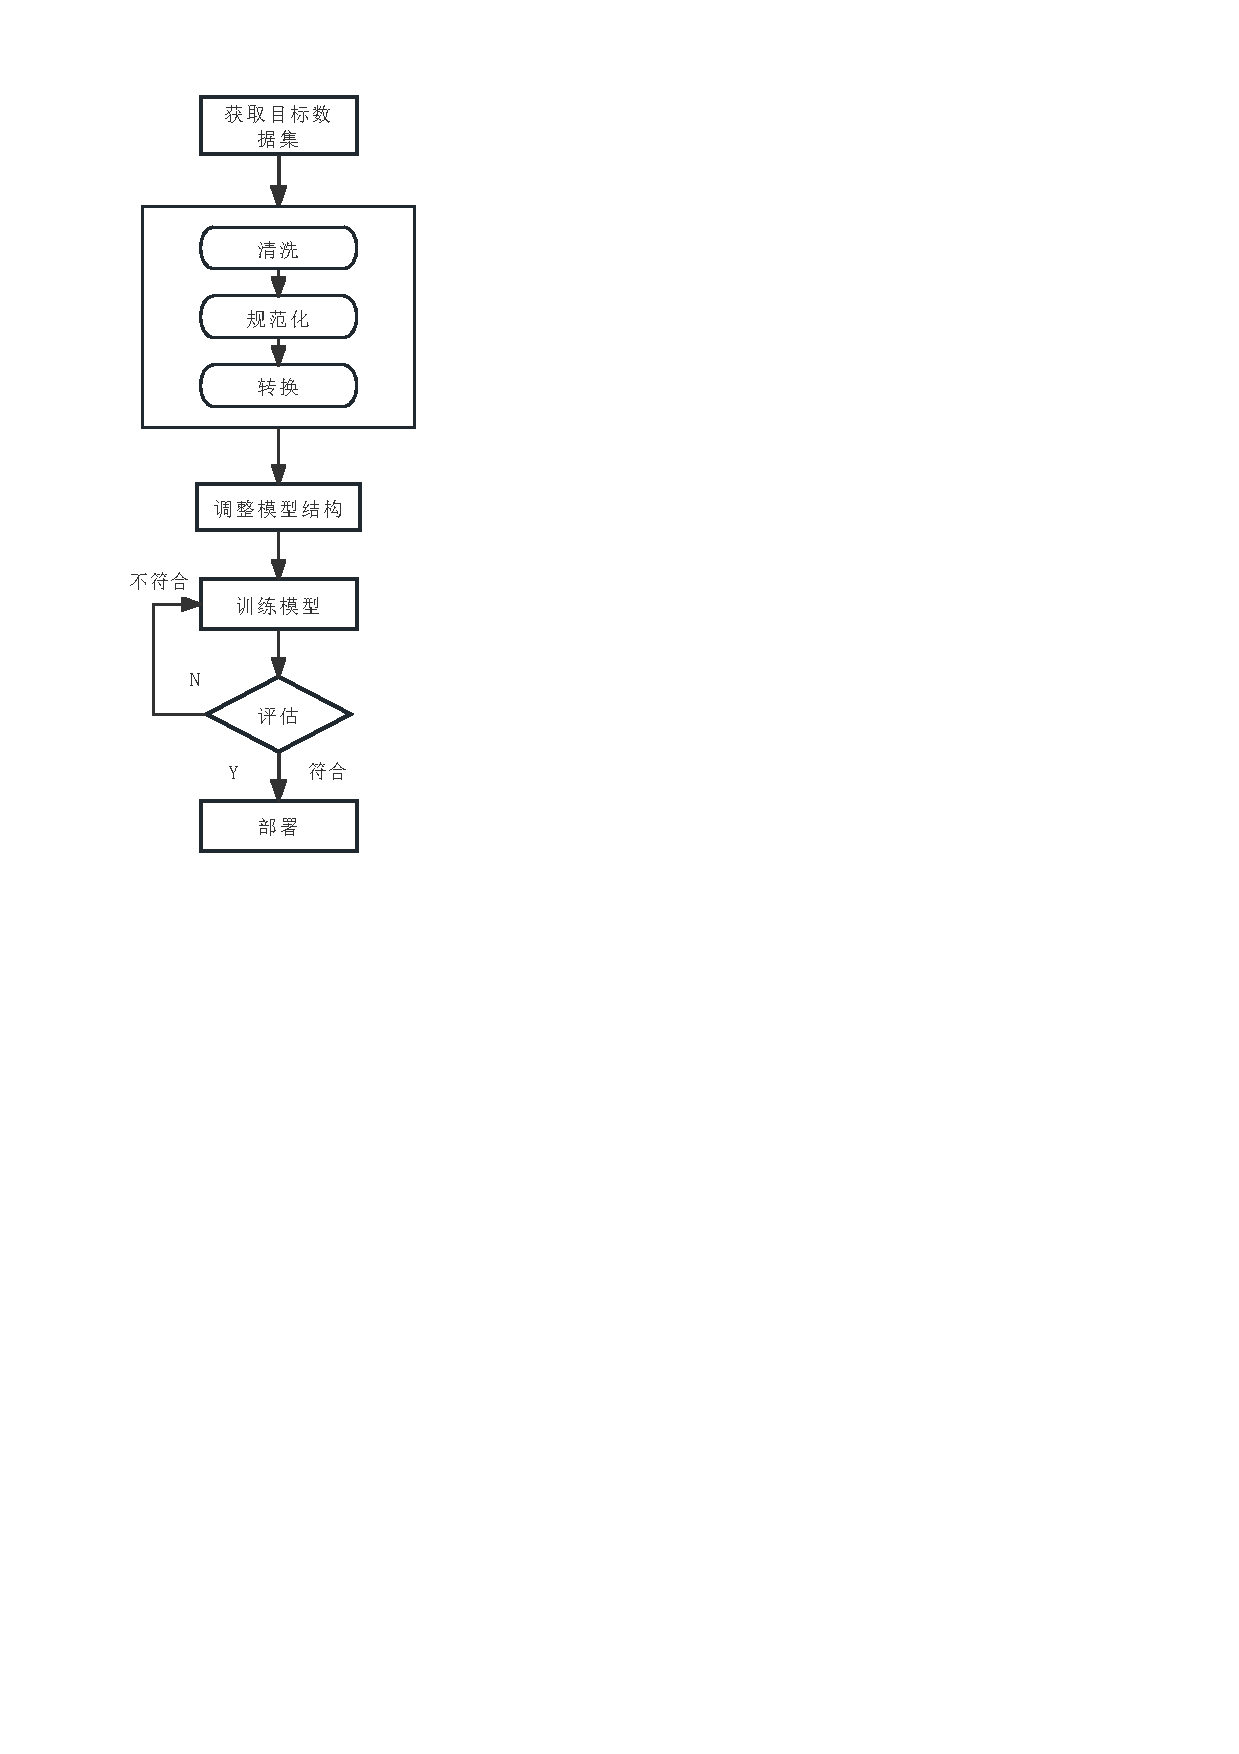
\includegraphics[height=.5\textheight,keepaspectratio]{img/transfer/transfer_method.pdf}
    \caption{迁移学习步骤}
    \label{fig:transfer_method}
\end{figure}
如图\ref{fig:transfer_method}示,将已在原数据集上训练好的模型,迁移到目标数据及步骤如下:
\begin{enumerate}
    \item 目标数据集预处理。预处理对于原始数据集几乎是必做的。在预处理中需要进行数据清洗去除不合理的样本。随后需要将样本中各属性值进行规范化,变换的目的是将数据转化为统一格式,以方便批量处理。最后还需要对样本进行转换,对数值进行转换一般会进行重映射,将数值分布调整到合适范围,以方便模型学习;对于非数值部分可以将其转化为数值,如自然语言处理中,会将单词转换为词向量。
    \item 随后需要将源数据集上训练得到的模型进行转换,以适应目标数据集。
    \item 转换后的模型会在目标数据集上进行训练,每次训练结束后都会进行评估,当模型符合实际需求就可部署到入侵检测系统中,不符合需求就会使用目标数据集进行进一步微调。
\end{enumerate}

\section{基于通用模型的迁移学习}
上述基于模型的信息学习方法最大的缺点已在绪论部分叙述,即没有充分利用数据集提供的信息,以辅助迁移学习过程。另一方面,不同数据集中一些属性的底层特征相同,然而迁移学习为了适应数据集维度的变化,将神经网络中的第1层删除,因此丢失可能对目标数据集有帮助的底层知识。

在前一章节构建了一种对时序建模的通用模型,该模型以数据集中对各属性描述的语义信息作为辅助。当该模型用于迁移学习时,解决了上述两个不足。

首先模型的第1阶段是Transformer编码器,该架构面向变长序列设计,因此具有良好的可扩展性,理论上可以兼容各种格式(不同维度)的输入。在更改数据集时,并不需要对第1层进行重置,对于多分类任务,只需重置最后一层用于分类的权重值。

因此使用通用模型进行迁移学习与使用传统模型进行迁移学习,在过程上有所不同。
\begin{enumerate}
    \item 目标数据集预处理。在使用通用模型进行迁移学习时,预处理仍然是必做的,特别是在第一步需要去除不合理的数据,以及第二步将数据集转化为标准格式,以适应模型的输入。随后需要将样本中各属性值进行重新映射,考虑到其通用性,一些对于数值属性的相对标准化方法可能不再适用。如最大最小值归一化。而使用其他相对标准化方式,如使用对数函数对数值进行变换,所有数值均使用一种函数,保留了各属性之间的相对重要程度。对于文本属性,将其转化为数字索引或独热编码并不合适,而应该使用词向量嵌入,使用前者进行编码,不同数据的同一文本可能会被编成不同形式,而使用后者进行编码,可保证同一文本被编码为同样的向量。
    \item 对于通用模型,数据集格式变化时,只需对模型进行轻微的调整,即在多分类任务中重置最后一层全连接层,二分类任务则不需要进行改动。
    \item 通过上述步骤转换后的模型会继续在目标数据集上进行训练,每次训练除了提供数据以及对应标签外,还需提供对该数据的描述文本信息,每次训练结束后进行评估,符合要求则进入部署阶段。
\end{enumerate}

在实际迁移学习训练过程中不会使用多个数据集,各类别描述在训练过程中为常量值。为节省计算量,可通过在初始化模型时将数据集中各属性的描述信息提前通过语言模型生成描述向量。因此在数据预处理步骤的文本编码过程中,除了对数据中的词建立词表还需对数据集各属性描述建立描述向量表。随后在第二步模型初始化过程中替换原有模型的词表以及描述向量表,即可完成模型迁移过程。

\subsection{迁移学习评估}
将KDDCUP-99数据集按照不同的比例进行划分,用以探究在不同数据量下模型迁移的效果。

如表\ref{tab:transfer-exp-acc}示本章提出的通用模型具有非常强的泛化能力,仅需0.02\%的数据即1024个数据包就可成功识别到所给定数据中的两类,而同样的传统模型,则只能识别到给定数据中数量最多的那一类,且模型过拟合。在数据量超过1\%后,模型的正确率也优于传统模型,仅数据量在1‰ $\sim$ 1\%时传统模型才优于本章提出的模型。
\begin{table}[htbp]
\caption{KDDCUP-99数据集上迁移能力评估实验}
    \centering
    \begin{adjustbox}{max width=\textwidth}
    \begin{tabular}{lllllllllllll}
    \toprule
        ~ & 数据& 使用量& 0.0001 &  0.0002&0.0005& 0.001& 0.002 & 0.005 & 0.01 & 0.02 & 0.05 & 0.1 \\ \midrule
        exp1 & acc & all & 0.7928 &  0.7928 &0.7653 & 0.7927 & 0.9888 & 0.9921 & 0.9921 & 0.9941 & 0.9964 & 0.9971 
\\ 
        exp2 & acc & all & 0.7928 &  0.8167 &0.9658 & 0.9564 & 0.9766 & 0.9957 & 0.9916 & 0.9948 & 0.9978 & 0.9982 \\
    \bottomrule
    \end{tabular}
    \end{adjustbox}
    \label{tab:transfer-exp-acc}
\end{table}

如表\ref{tab:transfer-exp-f1}示在数据量较少时传统模型直接对这些较少的类别判定为不存在(f1值为0),而本章提出的模型则正确识别到了这些类别即准确率大于个数最多的类别(拒绝服务)在模型中的占比。

\begin{table}[htbp]
\caption{KDDCUP-99数据集上迁移能力评估实验}
    \centering
    \begin{adjustbox}{max width=\textwidth}
    \begin{tabular}{lllllllllllll}
    \toprule
        ~ & 数据& 使用量& 0.0001 &  0.0002&0.0005& 0.001& 0.002 & 0.005 & 0.01 & 0.02 & 0.05 & 0.1 \\ \midrule
        exp1 & f1& BENIGN& 0.0000 &  0.2458 &0.9303 & 0.8908 & 0.9426 & 0.9912 & 0.9927 & 0.9914 & 0.9948 & 0.9958 
\\ 
        exp1 & f1& Probe& 0.0000 &  0.0000 &0.3764 & 0.7150 & 0.6904 & 0.7858 & 0.3115 & 0.7680 & 0.9352 & 0.9701 
\\
 exp1 & f1& Denial-of-Service& 0.8844 & 0.8965 & 0.9843 & 0.9744 & 0.9872 & 0.9989 & 0.9962 & 0.9979 & 0.9994 &0.9992 
\\
 exp1 & f1& U2R& 0.0000 & 0.0000 & 0.0000 & 0.0000 & 0.0000 & 0.0000 & 0.0000 & 0.0000 & 0.0202 &0.0000 
\\
 exp1 & f1
& R2L& 0.0000 & 0.0000 & 0.0000 & 0.0000 & 0.0000 & 0.0000 & 0.0010 & 0.0000 & 0.1739 &0.5116 
\\
 exp2 & f1& BENIGN& 0.0000 & 0.0000 & 0.9593 & 0.0000 & 0.9863 & 0.9900 & 0.9918 & 0.9884 & 0.9932 &0.9949 
\\
 exp2 & f1
& Probe& 0.0000 & 0.0000 & 0.0423 & 0.0000 & 0.1828 & 0.3647 & 0.4178 & 0.6531 & 0.8263 &0.9248 
\\
 exp2 & f1
& Denial-of-Service& 0.8844 & 0.8844 & 0.8320 & 0.8844 & 0.9958 & 0.9971 & 0.9965 & 0.9987 & 0.9990 &0.9991 
\\
 exp2 & f1& U2R& 0.0000 & 0.0000 & 0.0000 & 0.0000 & 0.0000 & 0.0000 & 0.0000 & 0.0000 & 0.0000 &0.0000 
\\
 exp2 & f1& R2L& 0.0000 & 0.0000 & 0.0000 & 0.0000 & 0.0000 & 0.0000 & 0.0073 & 0.0000 & 0.0000 &0.1732 
\\
    \bottomrule
    \end{tabular}
    \end{adjustbox}
    \label{tab:transfer-exp-f1}
\end{table}

将迁移后的结果与KDDCUP-99数据集上其他入侵检测方法比较,如表\ref{tab:compare_transfer_other}示,相比传统方式的迁移学习,使用通用模型进行迁移学习可达到更高准确率,多模态通用模型在实际网络安全场景中具有应用潜力。

\begin{table}[htbp]
    \centering
        \caption{KDDCUP-99数据集上与其他方法的对比}
    \begin{tabular}{lll}
    \toprule
        模型 & 数据集使用量 & 准确率 \\ \midrule
        基于通用模型的迁移学习& 0.1&99.82\%\\
        Hierarchical IDS\cite{10.3390/sym12020203} & 0.1 & 99.80\% \\
        基于非通用模型的迁移学习& 0.1&99.71\%\\
        CNID\cite{10.1155/2020/4705982}& 0.1 & 98.02\% \\
        FGLCC-CFA\cite{10.1016/j.jisa.2018.11.007}& 0.1 & 95.03\% \\
        \bottomrule
    \end{tabular}

    \label{tab:compare_transfer_other}
\end{table}

\subsection{可视化分析}


\begin{figure}[htbp] % 创建一个新的figure环境
\centering % 居中对齐所有的子图

\subfloat[训练后激活值分布情况]{ % 插入第一个子图及其标题
\begin{minipage}{.5\textwidth}
\centering % 居中对齐子图
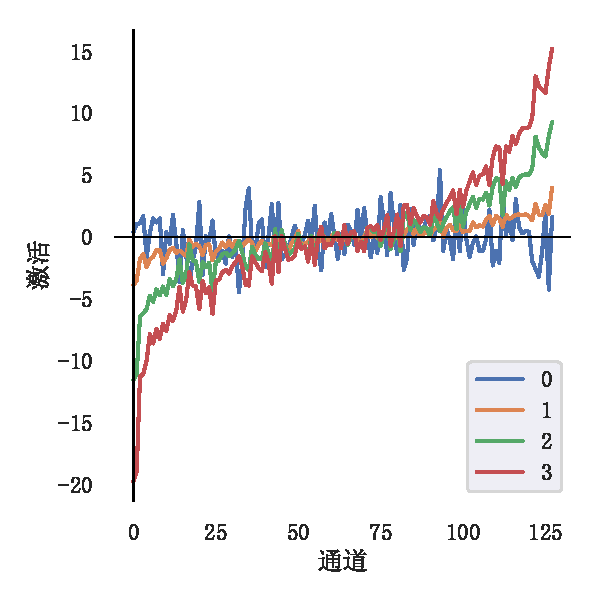
\includegraphics[width=1\linewidth]{img/transfer/activation_t.pdf} % 插入SVG图片
\label{fig:dist_t} % 子图的标签,用于交叉引用
\end{minipage}%
}
\subfloat[初始化时激活值分布情况]{ % 插入第二个子图及其标题
\begin{minipage}{.5\textwidth}
\centering
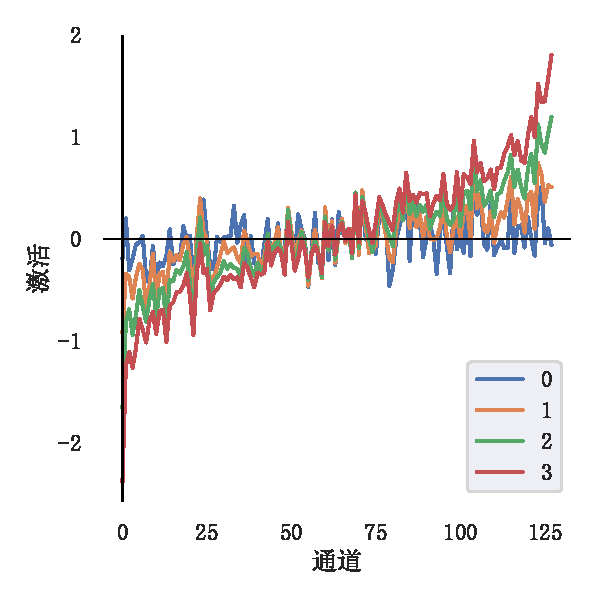
\includegraphics[width=1\linewidth]{img/transfer/activation_o.pdf} % 插入SVG图片
\label{fig:dist_o}
\end{minipage}
}

\subfloat[训练后激活值热图]{ % 插入第三个子图及其标题
\begin{minipage}{.5\textwidth}
\centering
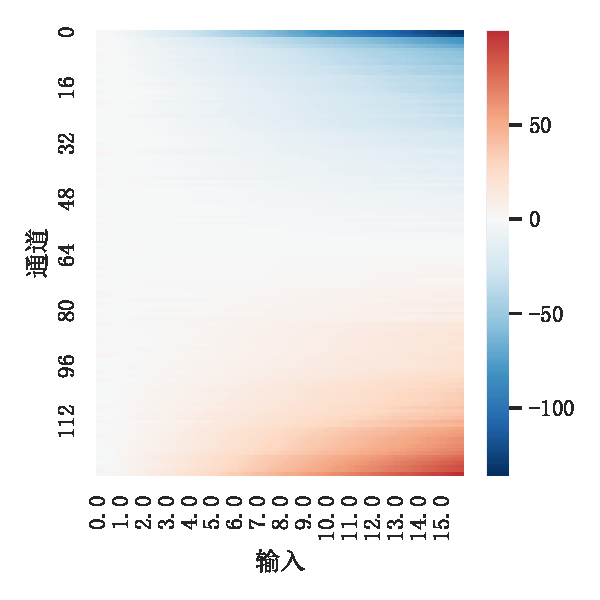
\includegraphics[width=1\linewidth]{img/transfer/channel_act_t.pdf} % 插入PNG图片
\label{fig:hot_t}
\end{minipage}%
}
\subfloat[初始化时激活值热图]{ % 插入第四个子图及其标题
\begin{minipage}{.5\textwidth}
\centering
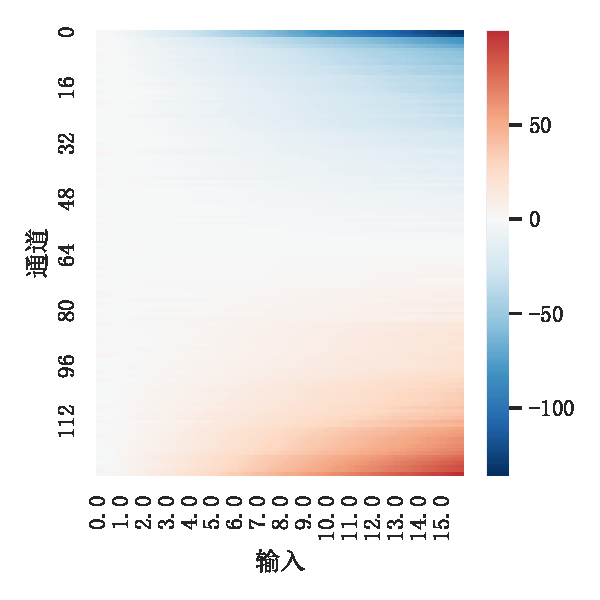
\includegraphics[width=1\linewidth]{img/transfer/channel_act_t.pdf} % 插入PNG图片
\label{fig:hot_o}
\end{minipage}
}

\caption{将数字转化为向量时各通道的激活值(按平均激活值排序)} % 四张图片作为整体的标题
\label{fig:activation_distribution_and_heatmap}
\end{figure}

在网络入侵检测数据集中存在两种数值,一种是分布范围为整个实数域的浮点数,另外一种就是百分比(表示是与否的真假值也可看作特殊百分比)取值范围是[0,1]区间。图\ref{fig:dist_o}与图\ref{fig:dist_t}分别表示初始化与完成训练时该编码器的激活值分布随输入值变化情况。可以看出训练后用于数值映射的多层感知机,成功识别到了这两种数值的不同,对于小于1的数值,多层感知机会将其映射为负的斜率,而将较大的数字往往映射为正的斜率,而且经过训练后,分布更为有序,激活值的绝对值大小扩大了近10倍。


\section{本章小结}

本章主要针对入侵检测模型,在实际部署中可能的困难进行研究。主要利用迁移学习克服因部署环境不同而导致已训练好的模型失效的问题。

对于实际部署环境中数据集格式的差别,常规模型使用基于模型微调的迁移学习方法,同时针对不同格式调整网络结构。对于前一章节提出的通用时序检测模型直接利用数据集中的描述信息提高迁移学习效果,同时由于其通用性,因此不必对网络结构进行调整。

实验结果中发现通用检测模型有较强的泛化能力,在少数据量时能避免模型过拟合,在多数据量时能超越传统迁移学习模型。最后通过与其他方法进行对比证明了基于时序的通用检测模型的有效性。
%%% mode: latex
%%% TeX-master: t
%%% End:

\chapter{总结与展望}
\label{cha:conclusion}

\section{本文主要内容及结论}
\label{sec:conclusion}
针对入侵检测领域的相关模型没有充分利用数据集中的描述信息,以及在迁移学习过程中当数据及格式发生变化时会丢弃较多已训练的参数,本文进行以下研究:

本研究提出了一种新的通用网络分类模型,主要由通用编码器以及时序建模层两部分组成。
第二章节主要讨论了数据预处理相关部分,针对模型的特点采取了合适的数据缩放方法以及提出了一种新的对流量序列进行数据增强的方法。
在第三章提出了一种基于多模态的通用编码器,对其设计进行了详细的阐述,该编码器可灵活适应各种格式的网络流量数据,同时将数据集中数据和描述信息融入其中,将其转变为统一格式的向量,通过实验验证了多模态的通用编码器的有效性。
在第四章节对通用网络分类模型的第二部分即时序建模进行深入分析与实验,提出并验证了一个有效的网络入侵检测模型,进一步证明编码器可有效改善时序模型在不均衡数据集上的性能,避免模型过拟合。也说明基于Transformer架构的网络与第三章节提出的通用编码器搭配最为合适。
在第五章节提出了一种基于通用时序检测模型的迁移学习,证明了其相比传统的基于模型迁移学习具有较强的迁移能力,且只需更改较少的网络结构,从而保留更多的已学习参数,仅需较少数据就可实现模型对新数据集中各类别的正确分类。与近期其他入侵检测相关工作相比本文提出的方法具有一定的先进性。提出的方案具有较高的实用价值。

\section{本文主要创新点}
\label{sec:contribution}
主要的创新点是解决了网络入侵中的关键问题,即公共数据集与实际部署环境中数据集的差异会导致模型性能下降。提出的解决方案是使用通用模型以及引入数据集文本描述信息进行辅助。辅助过程中使用BERT作为句子编码器,同时引入预计算过程,在保证编码器提取信息能力的同时降低计算量。

其次为了解决前一学习过程中数据多样性低的问题,提出了一种新的基于标签数据增强方法。该方法在对数据进行变换时,保持了网络流量数据之间的时序关系,提供了高质量的数据增强结果。

\section{本文存在的不足}

\begin{enumerate}

    \item 本文提出的是一个通用模型,但只在两个数据集上进行评估,所得结论有一定局限性,在更多数据集上进行测试,会更具有说服力。
    \item 机器学习除了用于防御也可用于攻击,评估模型对于对抗样本的鲁棒性也很重要,本文中的实验并未涉模型对对抗性样本的防御能力研究。
    \item  在模型结构中,通用编码器会对网络流量数据特征进行升维操作,会带来较大的计算量。
\end{enumerate}

\section{展望}
本文提出的模型还可进一步改进,可通过以下方法:
\begin{enumerate}
    \item 在通用编码器中引入降维操作,可使用传统方法也可以使用Transformer中的注意力机制实现。
    \item 可以开展更多的实验,评估本文提出的模型在计算效率等其他方面的表现。
    \item 现在已经有性能更好的语言模型如Llama 2,可使用这些大语言模型生成更合适的位置编码或者。
    \item 在模型的分类部分引入语义描述信息,有可能进一步提升模型对网络流量,特别是少样本流量的识别准确率,甚至还可能实现零样本分类。

\end{enumerate}



\label{sec:futurework}


%\input{body/chapter/cnn}
%\input{body/chapter/univ}

%%% 致谢

%%% Local Variables:
%%% mode: latex
%%% TeX-master: "../main"
%%% End:

\begin{ack}
首先,我要特别感谢吴俊军教授。吴老师在研究生期间给予了我无微不至的关怀和指导。无论是在生活上还是学习上,吴老师都始终站在我的身旁,为我提供宝贵的建议和支持。在我对研究生生活感到迷茫的时候,是吴老师为我指明了前进的方向。从吴老师身上,我不仅学到了专业知识,更学到了许多做人做事的道理。这些都将是我未来人生道路上最宝贵的财富。

同时,我要衷心感谢华科大网络空间安全学院的路松峰老师。路老师不仅以他深厚的学术造诣和严谨的治学态度。在路老师的悉心指导下,我得以参与到多个重要项目中,不仅锻炼了我的专业技能,也为我积累了宝贵的实践经验。从课题选题、实验设计到论文撰写修改,无不凝聚着老师的心血。在此,对路老师三年来给予我的悉心指导与关心表示最衷心的感谢,同时我衷心感谢各位授课老师的授业解惑与帮助,您们的悉心教育使我终身受益。

此外,我要感谢在“湖北省重点研发计划”项目中与我并肩作战的团队成员们。作为后端开发负责人,我深刻体会到团队合作的重要性。特别感谢那些在项目中给予我无私帮助和支持的同学们,你们的付出让我深受感动。

衷心感谢参与我论文评审和答辩的各位老师,你们的宝贵意见让我更加深入地认识到自己的不足,并为我指明了前进的方向。

衷心感谢学校和学院为我提供的丰富的学习资源、先进的实验条件和良好的学术氛围。

最后,我要感谢我的家人和朋友们。你们无尽的关爱和支持一直是我最坚实的后盾。正是如此,我才能够勇敢地面对挑战,坚定地走向未来。

感谢所有在我研究生生涯中给予我帮助和支持的人。你们的陪伴让我更加珍惜这段宝贵的时光,也让我对未来充满了信心和期待。

\end{ack}



%%% 参考文献
%Included for Gather Purpose only:
%input "ref/refs.bib"
\bibliographystyle{HUSTThesis}
\bibliography{ref/thesis}

% ---------------------------------------------

%%% 附录
\begin{appendix}
  %\input{body/appendix/app.tex}

\end{appendix}

\end{document}
